%%% DOCUMENTCLASS 
%%%-------------------------------------------------------------------------------

\documentclass[
a4paper, % Stock and paper size.
11pt, % Type size.
% article,
% oneside, 
onecolumn, % Only one column of text on a page.
% openright, % Each chapter will start on a recto page.
% openleft, % Each chapter will start on a verso page.
openany, % A chapter may start on either a recto or verso page.
]{memoir}

%%% PACKAGES 
%%%------------------------------------------------------------------------------

\usepackage[utf8x]{inputenc} % If utf8 encoding
% \usepackage[lantin1]{inputenc} % If not utf8 encoding, then this is probably the way to go
\usepackage[T1]{fontenc}    %
\usepackage[english]{babel} % English please
\usepackage[final]{microtype} % Less badboxes

% \usepackage{kpfonts} %Font

\usepackage{amsmath,amssymb,mathtools} % Math

% \usepackage{tikz} % Figures
\usepackage{graphicx} % Include figures

\usepackage{listings}    % Add code snippets
\usepackage[usenames,dvipsnames,svgnames,table]{xcolor}

\usepackage[linktocpage=true]{hyperref} % Extensive support for hypertext in LaTeX

\usepackage{dirtree} % Make directory trees easily
\usepackage{framed} % shade in a region of the page


%%% PAGE LAYOUT 
%%%------------------------------------------------------------------------------

\setlrmarginsandblock{0.15\paperwidth}{*}{1} % Left and right margin
\setulmarginsandblock{0.2\paperwidth}{*}{1}  % Upper and lower margin
\checkandfixthelayout

%%% SECTIONAL DIVISIONS
%%%------------------------------------------------------------------------------

\maxsecnumdepth{subsection} % Subsections (and higher) are numbered
\setsecnumdepth{subsection}

\makeatletter %
\makechapterstyle{standard}{
  \setlength{\beforechapskip}{0\baselineskip}
  \setlength{\midchapskip}{1\baselineskip}
  \setlength{\afterchapskip}{8\baselineskip}
  \renewcommand{\chapterheadstart}{\vspace*{\beforechapskip}}
  \renewcommand{\chapnamefont}{\centering\normalfont\Large}
  \renewcommand{\printchaptername}{\chapnamefont \@chapapp}
  \renewcommand{\chapternamenum}{\space}
  \renewcommand{\chapnumfont}{\normalfont\Large}
  \renewcommand{\printchapternum}{\chapnumfont \thechapter}
  \renewcommand{\afterchapternum}{\par\nobreak\vskip \midchapskip}
  \renewcommand{\printchapternonum}{\vspace*{\midchapskip}\vspace*{5mm}}
  \renewcommand{\chaptitlefont}{\centering\bfseries\LARGE}
  \renewcommand{\printchaptertitle}[1]{\chaptitlefont ##1}
  \renewcommand{\afterchaptertitle}{\par\nobreak\vskip \afterchapskip}
}
\makeatother

\chapterstyle{standard}

\setsecheadstyle{\normalfont\large\bfseries}
\setsubsecheadstyle{\normalfont\normalsize\bfseries}
\setparaheadstyle{\normalfont\normalsize\bfseries}
\setparaindent{0pt}\setafterparaskip{0pt}

%%% FLOATS AND CAPTIONS
%%%------------------------------------------------------------------------------

\makeatletter                  % You do not need to write [htpb] all the time
\renewcommand\fps@figure{htbp} %
\renewcommand\fps@table{htbp}  %
\makeatother                   %

\captiondelim{\space } % A space between caption name and text
\captionnamefont{\small\bfseries} % Font of the caption name
\captiontitlefont{\small\normalfont} % Font of the caption text

\changecaptionwidth          % Change the width of the caption
\captionwidth{1\textwidth} %

%%% ABSTRACT
%%%------------------------------------------------------------------------------

\renewcommand{\abstractnamefont}{\normalfont\small\bfseries} % Font of abstract title
\setlength{\absleftindent}{0.1\textwidth} % Width of abstract
\setlength{\absrightindent}{\absleftindent}

%%% HEADER AND FOOTER 
%%%------------------------------------------------------------------------------

\makepagestyle{standard} % Make standard pagestyle

\makeatletter                 % Define standard pagestyle
\makeevenfoot{standard}{}{}{} %
\makeoddfoot{standard}{}{}{}  %
\makeevenhead{standard}{\bfseries\thepage\normalfont\qquad\small\leftmark}{}{}
\makeoddhead{standard}{}{}{\small\rightmark\qquad\bfseries\thepage}
% \makeheadrule{standard}{\textwidth}{\normalrulethickness}
\makeatother                  %

\makeatletter
\makepsmarks{standard}{
\createmark{chapter}{both}{shownumber}{\@chapapp\ }{ \quad }
\createmark{section}{right}{shownumber}{}{ \quad }
\createplainmark{toc}{both}{\contentsname}
\createplainmark{lof}{both}{\listfigurename}
\createplainmark{lot}{both}{\listtablename}
\createplainmark{bib}{both}{\bibname}
\createplainmark{index}{both}{\indexname}
\createplainmark{glossary}{both}{\glossaryname}
}
\makeatother                               %

\makepagestyle{chap} % Make new chapter pagestyle

\makeatletter
\makeevenfoot{chap}{}{\small\bfseries\thepage}{} % Define new chapter pagestyle
\makeoddfoot{chap}{}{\small\bfseries\thepage}{}  %
\makeevenhead{chap}{}{}{}   %
\makeoddhead{chap}{}{}{}    %
% \makeheadrule{chap}{\textwidth}{\normalrulethickness}
\makeatother

\nouppercaseheads
\pagestyle{standard}               % Choosing pagestyle and chapter pagestyle
\aliaspagestyle{chapter}{chap} %

%%% NEW COMMANDS
%%%------------------------------------------------------------------------------
% custom constants defined in here
% ----------------------------------------------------------------------
% Program constants that can be changed through-out the document
% ----------------------------------------------------------------------

% This sets the header value for the time in calibDB
\newcommand{\constantAcqtimeKey}{ACQTIME1}

% This sets the folder name date format
\newcommand{\constantFolderDateFormat}{YYYYMMDD}

\newcommand{\MyVersion}{0.0.4}

\newcommand{\MyDate}{2017-11-10}

\newcommand{\MyAuthors}{F. Bouchy, E. Artigau, I. Boisse, N. Cook, M. Hobson, C. Moutou}








% custom commands defined in here
% ----------------------------------------------------------------------
% formatting constants
% ----------------------------------------------------------------------
% formatting the named variables (from user setup)
\newcommand{\definevariable}[1]{\textcolor{blue}{\{#1\}}}
% formatting the named keywords 
\newcommand{\definekeyword}[1]{\textcolor{red}{\{#1\}}}
% formatting the TODO command
\newcommand{\TODO}[1]{\vspace{0.5cm}\colorbox{black}{\parbox{0.9\textwidth}{\textcolor{green}{!!!! TODO !!!! #1 !!!!}}}\vspace{0.5cm}}

% formatting for the directories trees
\newcommand{\customdirtree}[1]{
\vspace{-0.25cm}
\definecolor{shadecolor}{rgb}{0.85,0.85,0.82}
\begin{shaded}
\renewcommand*\DTstylecomment{\ttfamily\textcolor{black}}
\renewcommand*\DTstyle{\ttfamily\textcolor{blue}}
\dirtree{%
#1}
\end{shaded}
}
 


\newcommand{\p}{\partial} %Partial
% Or what ever you want

%%% TABLE OF CONTENTS
%%%------------------------------------------------------------------------------

\maxtocdepth{subsection} % Only parts, chapters and sections in the table of contents
\settocdepth{subsection}

\AtEndDocument{\addtocontents{toc}{\par}} % Add a \par to the end of the TOC

%%% INTERNAL HYPERLINKS
%%%-------------------------------------------------------------------------------

\usepackage{hyperref}   % Internal hyperlinks
\hypersetup{
    pdfauthor={Neil Cook},
    pdfcreator={Neil Cook},
    pdftitle={SPIRou User Manual},
    pdfsubject={SPIRou DRS},
    pdfkeywords={SPIRou, DRS, Pipeline},
    colorlinks=true,         % false: boxed links; true: colored links
    linkcolor=blue,          % color of internal links (change box color with linkbordercolor)
    citecolor=Maroon,        % color of links to bibliography
    filecolor=blue,          % color of file links
    urlcolor=blue,           % color of external links
    plainpages=false,       
}
\usepackage{memhfixc}   %

% get code highlighting parameters
\definecolor{codegreen}{rgb}{0,0.6,0}
\definecolor{codegray}{rgb}{0.5,0.5,0.5}
\definecolor{codepurple}{rgb}{0.58,0,0.82}

\definecolor{backcolour1}{rgb}{0.95,0.95,0.92}
\definecolor{backcolour2}{rgb}{1,0.977,0.801}
\definecolor{backcolour3}{rgb}{0.79,0.88,1}

\lstdefinestyle{text}{
    backgroundcolor=\color{backcolour1},   
    commentstyle=\color{codegreen},
    keywordstyle=\color{magenta},
    numberstyle=\tiny\color{codegray},
    stringstyle=\color{codepurple},
    basicstyle=\ttfamily\scriptsize,
    breakatwhitespace=false,         
    breaklines=true,                 
    captionpos=b,                    
    keepspaces=true,                 
    % numbers=left,                    
    % numbersep=5pt,                  
    showspaces=false,                
    showstringspaces=false,
    showtabs=false,                  
    tabsize=2,
    moredelim=**[is][\color{red}]{@}{@},
    moredelim=**[is][\color{OliveGreen}]{<}{>},
    extendedchars=false,
    columns=fullflexible,
	literate={\\@}{{\unichar{"0040}}}1
			 {\\<}{{\unichar{"003C}}}1 
			 {\\>}{{\unichar{"003E}}}1
}

\lstdefinestyle{bashstyle}{
	language=bash,
    backgroundcolor=\color{backcolour2},   
    commentstyle=\color{codegreen},
    keywordstyle=\color{magenta},
    numberstyle=\tiny\color{codegray},
    stringstyle=\color{codepurple},
    basicstyle=\ttfamily\scriptsize,
    breakatwhitespace=false,         
    breaklines=true,                 
    captionpos=b,                    
    keepspaces=true,                 
    % numbers=left,                    
    % numbersep=5pt,                  
    showspaces=false,                
    showstringspaces=false,
    showtabs=false,                  
    tabsize=2,
    moredelim=**[is][\color{red}]{@}{@},
    extendedchars=false,
    columns=fullflexible,
    literate={\\@}{{\unichar{"0040}}}1
}

\lstdefinestyle{pythonstyle}{
    language=Python,
    backgroundcolor=\color{backcolour3},   
    commentstyle=\color{codegreen},
    keywordstyle=\color{magenta},
    numberstyle=\tiny\color{codegray},
    stringstyle=\color{codepurple},
    basicstyle=\ttfamily\scriptsize,
    breakatwhitespace=false,         
    breaklines=true,                 
    captionpos=b,                    
    keepspaces=true,                 
    % numbers=left,                    
    % numbersep=5pt,                  
    showspaces=false,                
    showstringspaces=false,
    showtabs=false,                  
    tabsize=2,
    moredelim=**[is][\color{red}]{@}{@},
    extendedchars=false,
    columns=fullflexible,
    literate={\\@}{{\unichar{"0040}}}1
}

%%% THE DOCUMENT
%%% Where all the important stuff is included!
%%%-------------------------------------------------------------------------------

\author{N. Cook}
\title{{\Huge SPIRou User Manual} \\ {\small Version 0.0.1}}
\date{2017-10-19}

% \usepackage{lipsum} % Just to put in some text

\begin{document}

\frontmatter

\maketitle

% Add logo to title page
\vspace{2cm}
\begin{center}

\includegraphics[width=.5\textwidth]{figures/Logo_SPIRou-22.pdf}
\end{center}
\vspace{2cm}

\begin{abstract}
This is the guide to installing, running, and using the SPIRou DRS.
\end{abstract}
\clearpage

\tableofcontents*
\clearpage

% Introduction
\chapter{Introduction}

Some text here

\section{Notes}
\begin{itemize}
\item This installation assumes you are running bash on a Linux machine.

\item There is no need for root access needed for any of these steps.

\item The python modules required for this DRS to run (more up-to-date versions are NOT supported) will make current versions of python not work. It is currently recommended that an isolated version of python be used with this version of the DRS (see Section \ref{section:install-python}).

\item Variables inside \definevariable{ } are defined in Section \ref{section:edit_env_setup} and used throughout to mean ``replace with valued defined in Section \ref{section:edit_env_setup}''.

\item The following denotes a line of text that is to be edited (in a file):

\begin{lstlisting}[style=text]
@VARIABLE_NAME@="Variable Value"
\end{lstlisting}

\item The following denotes a console command to run:

\begin{lstlisting}[language=bash, style=bashstyle]
echo "HelloWorld!"
\end{lstlisting}


\item The following denotes a python command to run:


\begin{lstlisting}[language=Python, style=pythonstyle]
>>> print("HelloWorld!")
\end{lstlisting}

\end{itemize}


%%%-------------------------------------------------------------------------------
\mainmatter
% Define the chapters here
%%%-------------------------------------------------------------------------------

% Chapter 1: Pre-Installation guide
% ---------------------------------------------------------------------
\chapter{Pre-Installation}
% ---------------------------------------------------------------------

This file is just for use with the current installation files (version 43), the author does not recommend that this is the final set-up procedure, nor that any of the `modifications' to the original source code applied here should be used in any final version of the DRS (better solutions should be found). \\



% ---------------------------------------------------------------------
\section{Prerequisites}
% ---------------------------------------------------------------------

Before one can use the DRS pipeline one must follow the followings steps before installing the pipeline.

\begin{enumerate}
\item Add variables to the system environment (Section \ref{section:edit_env_setup})
\item Setup and check the folder structure (Section \ref{section:folder_setup})
\item Make sure Fortran and C back-ends are installed (Section \ref{section:fortran_gsl})
\item Install an isolated, clean version of python (Section \ref{section:install-python})
\item Install required python modules - exact version not older not newer (Section \ref{section:install-py-modules})
\end{enumerate}

\noindent There is no need for root access for any of the following steps.

% ---------------------------------------------------------------------
\section{Adding variables to the system environment}
\label{section:edit_env_setup}
% ---------------------------------------------------------------------

This can be done one of two ways. The first root (Section \ref{section:using_setup_sh}) is via a setup file and will allow you to switch on and switch of the environmental variables (to avoid clashes with other programs and to keep ones environment clean). Note with this method you will have to source the setup script before installing or running this code (each time the environment changes) or add the activation to your bashrc. This route is recommended. Otherwise you can follow the second root (Section \ref{section:using_bashrc}) and hard-code variables to your `.bashrc' file.

\subsection{Using a setup script}
\label{section:using_setup_sh}

\noindent Open up `env\_setup.sh' and edit the following lines. You will find a copy of `env\_setup.sh' in Appendix \ref{section:source_code_env_setup_sh}.

\begin{enumerate}
\item Set the instrument name \definevariable{INSTRUMENT\_NAME}
\item Directory in which all SPIROU files go \definevariable{DATA\_ROOT}
\item Define installation folder name \definevariable{INSTALL\_ROOT}
\item Define data folder name \definevariable{DATA\_ROOT}
\item Define raw path \definevariable{DATA\_ROOT\_RAW}
\item Define reduced path \definevariable{DATA\_ROOT\_REDUCED}
\item Define calibDB path \definevariable{DATA\_ROOT\_CALIB}
\item Define msg path \definevariable{DATA\_ROOT\_MSG}
\item Define tmp path \definevariable{DATA\_ROOT\_TMP}
\item Define python version \definevariable{PYTHON\_VERSION}
\item Define python directory (i.e. result of command "which python") \definevariable{PYTHON\_DIR}
\item Define GSL path (default paths if installed may be /usr/local/include/gsl or /opt/gsl) \definevariable{GSL\_DIR}
\end{enumerate}

\noindent i.e. these lines in `env\_setup.sh'.

\begin{lstlisting}[style=text]
<INSTRUMENT_NAME>="SPIROU"
<DIR>="/data/spirou/drs"
<INSTALL_ROOT>="@$DIR@/INTROOT"
<DATA_ROOT>="@$DIR@/data"
<DATA_RAW_ROOT>="@$DATA_ROOT@/raw/"
<DATA_ROOT_REDUCED>="@$DATA_ROOT@/reduced/"
<DATA_ROOT_CALIB>="@$DATA_ROOT@/calibDB"
<DATA_ROOT_MSG>="@$DATA_ROOT@/msg/"
<DATA_ROOT_TMP>="@$DATA_ROOT@/tmp/"
<PYTHON_VERSION>="2.7"
<PYTHON_DIR>="@$DIR@/python/miniconda2/"
<GSL_DIR>="@$DIR@/c-libraries/gsl"
\end{lstlisting}

\noindent where any pre-defined variable can be used with a preceding \$ sign (to avoid repetition - coloured above in red).


\subsection{Adding variables to .bashrc file}
\label{section:using_bashrc}

Open `\~\/.bashrc' in your favourite text editor.

Add the following to it:
\begin{lstlisting}[style=text]
    
  @export@ INSTRUMENT={INSTRUMENT_NAME}
  @export@ DRS_DATA_RAW={DATA_ROOT_RAW}
  @export@ DRS_DATA_REDUC={DATA_ROOT_REDUCED}
  @export@ DRS_CALIB_DB={DATA_ROOT_CALIB}
  @export@ DRS_DATA_MSG={DATA_ROOT_MSG}
  @export@ DRS_DATA_WORKING={DATA_ROOT_TMP}
  @export@ TDATA={DATA_ROOT}

  @export@ INTROOT={INSTALL_ROOT}
  @export@ PATH={INSTALL_ROOT}/bin:{PYTHON_DIR}/bin/:$PATH
  @export@ PYTHONPATH=.:{PYTHON_DIR}/lib/python{PYTHON_VERSION}/site-packages/:{INSTALL_ROOT}/bin
  @export@ DRS_LOG=1
  @export@ PYTHON_INCLUDE_DIR="{PYTHON_DIR}/lib/python{PYTHON_VERSION}/site-packages/numpy/core/include"
  @export@ GSL_INCLUDE_DIR={GSL_DIR}/include
  @export@ GSL_LIBRARY_DIR={GSL_DIR}/lib

  @chmod@ +x "$PYTHON_DIR/bin/conda"
  @alias@ conda="$PYTHON_DIR/bin/conda"
  @chmod@ +x "$PYTHON_DIR/bin/pip"
  @alias@ pip="$PYTHON_DIR/bin/pip"
  @chmod@ +x "$PYTHON_DIR/bin/f2py"
  @alias@ f2py="$PYTHON_DIR/bin/f2py"

\end{lstlisting}

where:

\begin{itemize}
\item \definevariable{INSTRUMENT\_NAME} = Set the instrument name
\item \definevariable{DATA\_ROOT}= Directory in which all SPIROU files go
\item \definevariable{INSTALL\_ROOT} = Define installation folder name
\item \definevariable{DATA\_ROOT} = Define data folder name
\item \definevariable{DATA\_ROOT\_RAW} = Define raw path
\item \definevariable{DATA\_ROOT\_REDUCED} Define reduced path
\item \definevariable{DATA\_ROOT\_CALIB} = Define calibDB path
\item \definevariable{DATA\_ROOT\_MSG} = Define msg path
\item \definevariable{DATA\_ROOT\_TMP} = Define tmp path
\item \definevariable{PYTHON\_VERSION} = Define python version
\item \definevariable{PYTHON\_DIR} = Define python directory (i.e. result of command "which python")
\item \definevariable{GSL\_DIR} = Define GSL path (default paths if installed may be /usr/local/include/gsl or /opt/gsl)
\end{itemize}

\noindent Note: you will have to remove all these environmental variables/aliases to use any other version of python on your system.

% ---------------------------------------------------------------------
\section{Setup up and check file structure}
\label{section:folder_setup}
% ---------------------------------------------------------------------

Make sure the following folders are created:

\begin{lstlisting}[style=bashstyle]
@mkdir@ {DIR}
@mkdir@ {DIR}/{INSTALL_ROOT}/bin
@mkdir@ {DATA_ROOT}
@mkdir@ {DATA_RAW_ROOT}
@mkdir@ {DATA_ROOT_REDUCED}
@mkdir@ {DATA_ROOT_CALIB}
@mkdir@ {DATA_ROOT_MSG}
@mkdir@ {DATA_ROOT_TMP}
\end{lstlisting}

\noindent i.e. for the above `env\_setup.sh' this would be

\begin{lstlisting}[style=bashstyle]
@mkdir@ "/data/spirou/drs"
@mkdir@ "/data/spirou/drs/INTROOT/bin"
@mkdir@ "/data/spirou/drs/data"
@mkdir@ "/data/spirou/drs/data/raw"
@mkdir@ "/data/spirou/drs/data/reduced"
@mkdir@ "/data/spirou/drs/data/calibDB"
@mkdir@ "/data/spirou/drs/data/msg"
@mkdir@ "/data/spirou/drs/data/tmp"
\end{lstlisting}

% ---------------------------------------------------------------------
\section{Fortran and C back-end installation}
\label{section:fortran_gsl}
% ---------------------------------------------------------------------

% ---------------------------------------------------------------------
\subsection{Checking Fortran/C back-ends}
\label{section:checking for Fortran/C}
% --------------------------------------------------------------------

\TODO{design checks for Fortran and C, or do we just say that \\ installation requires Fortran and C to be install \\(Installing Fortran and C will require root access).}

Please check whether Fortran and C are installed. In addition to C you will need the C package `GSL', check that it is installed (default paths may be: /usr/local/include/gsl or /opt/gsl). If it is not installed please follow the instructions in Section \ref{section:install-gsl}.

% ---------------------------------------------------------------------
\subsection{Installing GSL back-ends without root access}
\label{section:install-gsl}
% ---------------------------------------------------------------------

To install GSL without root us the following steps:

\begin{enumerate}
\item download from \url{http://ftpmirror.gnu.org/gsl/}

\begin{lstlisting}[style=bashstyle]
@wget@ http://ftpmirror.gnu.org/gsl/gsl-1.16.tar.gz
\end{lstlisting}

\item create the \definevariable{GSL\_DIR} (from above)
\begin{lstlisting}[style=bashstyle]
@mkdir@ {GSL_DIR}
\end{lstlisting}

\item untar the GSL files
\begin{lstlisting}[style=bashstyle]
@tar@ -xvf gs1-1.16.tar.gz
\end{lstlisting}

\item change to untarred directory
\begin{lstlisting}[style=bashstyle]
@cd@ gs1-1.16/
\end{lstlisting}

\item configure the installation dir for GSL
\begin{lstlisting}[style=bashstyle]
./configure prefix={GSL_DIR}
\end{lstlisting}

\item build the GSL installation
\begin{lstlisting}[style=bashstyle]
make
\end{lstlisting}

\item install the GSL installation
\begin{lstlisting}[style=bashstyle]
make install
\end{lstlisting}

\end{enumerate}

% ---------------------------------------------------------------------
\section{Install isolated version of Python}
\label{section:install-python}
% ---------------------------------------------------------------------

As the current DRS requires specific versions of modules to run we recommend a isolated version of python (as to not interfere with your system or running other python codes). 

\noindent Python installation must meet the following specifications:

\begin{itemize}
\item  numpy 1.8.2 (versions later than 1.8.2 are unsupported)
\item  scipy 0.14
\item  matplotlib 1.3.1
\item  pyfits 3.2.4 
\end{itemize}

\noindent Hence installing Miniconda (a minimal version of the anaconda python distribution) is the easiest way to achieve this in an isolated environment (as not to destroy any current/system version of python). See section \ref{section:install-miniconda} for Miniconda install instructions.


% -------------------------------------------------------------------------------------------
\subsection{Installing Miniconda}
\label{section:install-miniconda}
% -------------------------------------------------------------------------------------------

To install Miniconda follow the steps below:

\begin{enumerate}
\item  download miniconda from here: https://conda.io/miniconda.html
\begin{lstlisting}[style=bashstyle]
@wget@ https://repo.continuum.io/miniconda/Miniconda2-latest-Linux-x86_64.sh
\end{lstlisting}


\item  run bash script
\begin{lstlisting}[style=bashstyle]
@bash@ Miniconda2-latest-Linux-x86_64.sh
\end{lstlisting}


\noindent Note: choose Miniconda installation directory to match \definevariable{PYTHON\_DIR} above
\noindent Note: if you wish to activate this environment/use other python installations do not add Miniconda2 install location to PATH in \~/.bashrc
          
\item  add \definevariable{PYTHON\_DIR} to FRONT of PATH environment (temporarily).
\begin{lstlisting}[style=bashstyle]
@export@ PATH={PYTHON_DIR}/bin:$PATH
\end{lstlisting}



\item  check that we are using the correct version of python/conda/pip
\begin{lstlisting}[style=bashstyle]
@which@ python
\end{lstlisting}


      
Should read: 
\begin{lstlisting}[style=bashstyle]
{PYTHON_DIR}/bin/python 
\end{lstlisting}


\noindent or 
\begin{lstlisting}[style=bashstyle]
{PYTHON_DIR}/bin/python{PYTHON_VERSION} 
\end{lstlisting}


\noindent similarly for
\begin{lstlisting}[style=bashstyle]
@which@ conda
@which@ pip
\end{lstlisting}

\noindent which should read:
\begin{lstlisting}[style=bashstyle]
{PYTHON_DIR}/bin/conda  
\end{lstlisting}

\noindent and 
\begin{lstlisting}[style=bashstyle]
{PYTHON_DIR}/bin/pip respectively
\end{lstlisting}

\end{enumerate}



% ---------------------------------------------------------------------
\section{Install required python modules}
\label{section:install-py-modules}
% ---------------------------------------------------------------------

\subsection{Installation}

\begin{enumerate}
\item  install numpy with miniconda
\begin{lstlisting}[style=bashstyle]
@conda@ install numpy==1.8.2
\end{lstlisting}
\begin{lstlisting}[style=bashstyle]
Fetching package metadata .........
Solving package specifications: .

Package plan for installation in environment /scratch/bin/miniconda2/test:

The following NEW packages will be INSTALLED:

    libgfortran: 1.0-0
    numpy:       1.8.2-py27_1

The following packages will be UPDATED:

    conda:       4.3.21-py27_0 --> 4.3.27-py27hff99c7a_0

          Proceed ([y]/n)? y
\end{lstlisting}

          
\item  install scipy with miniconda
\begin{lstlisting}[style=bashstyle]
@conda@ install scipy==0.14
\end{lstlisting}
\begin{lstlisting}[style=bashstyle]
Fetching package metadata ...........
Solving package specifications: .

Package plan for installation in environment /scratch/bin/miniconda2/test:

The following NEW packages will be INSTALLED:

    scipy:     0.14.0-np18py27_0

The following packages will be UPDATED:

    conda-env: 2.6.0-0           --> 2.6.0-h36134e3_1


          Proceed ([y]/n)? y
\end{lstlisting}

\item  install matplotlib with miniconda
\begin{lstlisting}[style=bashstyle]
@conda@ install matplotlib==1.3.1
\end{lstlisting}
\begin{lstlisting}[style=bashstyle]
Fetching package metadata ...........
Solving package specifications: .

Package plan for installation in environment /scratch/bin/miniconda2/test:

The following NEW packages will be INSTALLED:

    cairo:      1.12.18-0
    dateutil:   2.4.1-py27_0
    freetype:   2.4.10-0
    libpng:     1.5.13-1
    matplotlib: 1.3.1-np18py27_1
    pixman:     0.26.2-0
    py2cairo:   1.10.0-py27_2
    pyqt:       4.10.4-py27_0
    pytz:       2017.2-py27hcac29fa_1
    qt:         4.8.5-0
    sip:        4.15.5-py27_0

The following packages will be DOWNGRADED:

    pyparsing:  2.1.4-py27_0          --> 2.0.1-py27_0

            
        Proceed ([ y ]/ n ) ? y

\end{lstlisting}

\item  download pyfits 3.2.4 from \url{http://www.stsci.edu/institute/software_hardware/pyfits/Download}
\begin{lstlisting}[style=bashstyle]
@wget@ https://pypi.python.org/packages/source/p/pyfits/pyfits-3.2.4.tar.gz
\end{lstlisting}

\item  install pyfits with pip
\begin{lstlisting}[style=bashstyle]
@pip@ install pyfits-3.2.4.tar.gz
\end{lstlisting}

\end{enumerate}


% ----------------------------------------------------------------
\subsection{Checking installed module versions}
\label{section:check-versions}
% ----------------------------------------------------------------

Before we continue we should check python and module installation.

\begin{enumerate}
\item  run python
          
\begin{lstlisting}[style=bashstyle]
@python@
\end{lstlisting}

\noindent Inside python run following commands
\begin{lstlisting}[style=pythonstyle]
>>> @import@ numpy
>>> @import@ matplotlib
>>> @import@ scipy
>>> @import@ pyfits
\end{lstlisting}


\noindent Test the version with:
\begin{lstlisting}[style=pythonstyle]
>>> numpy.__version__
1.8.2
>>> matplotlib.__version__
1.3.1
>>> scipy.__version__
0.14.0
>>> pyfits.__version__
3.2.4
\end{lstlisting}

\end{enumerate}

% Chapter 2: Installation guide
% ---------------------------------------------------------------------
\chapter{Installation}
% ---------------------------------------------------------------------

This is just for use with the current installation files (version 43), the author does not recommend that this is the final set-up procedure, nor that any of the `modifications' to the original source code applied here should be used in any final version of the DRS (better solutions should be found). \\


% ---------------------------------------------------------
\section{Activate environment}
\label{section:activate}
% ---------------------------------------------------------

If you followed the steps in \ref{section:using_setup_sh} please follow this section, if however you followed the steps in \ref{section:using_bashrc} continue to Section \ref{section:downloading_install_Scripts}.

\noindent Before running the installation (or before running the code) one must run the following:
\begin{lstlisting}[style=bashstyle]
@source@ env_setup.sh
\end{lstlisting}

\noindent Output should look like this:
\begin{lstlisting}[style=bashstyle]
  =========================================
    Environmental setup for SPIRou Pipeline
  =========================================
    Setting up environment
    Set up for {INSTRUMENT}
      - Python located at: {PYTHON_DIR}
      - GLS located at: {GSL_DIR}
      - data located at:
            {DATA_ROOT}
            {DATA_RAW_ROOT}
            {DATA_ROOT_REDUCED}
            {DATA_ROOT_CALIB}
            {DATA_ROOT_MSG}
            {DATA_ROOT_TMP}

    Done
\end{lstlisting}

\noindent Note to deactivate type
\begin{lstlisting}[style=bashstyle]
@source@ env_setup.sh --clean
\end{lstlisting}


% ---------------------------------------------------------
\section{Downloading the preparing the install scripts}
\label{section:downloading_install_Scripts}
% ---------------------------------------------------------

Minor modifications need to be made to the code to allow a isolated version of GSL to be used. If and only if your GSL is installed to `/opt/gsl/' will the code install correctly with out this modification. The other steps are as in the original installation procedure. \\

\begin{enumerate}
\item change directory to \definevariable{DIR}
\begin{lstlisting}[style=bashstyle]
{DIR}
\end{lstlisting}

\item download source code for spirou, location should be \definevariable{DIR}/spirou
\begin{lstlisting}[style=bashstyle]
svn co https://svn.lam.fr/repos/spirou/trunk spirou
\end{lstlisting}

\end{enumerate}

\begin{enumerate}
\item change directory to source files
\begin{lstlisting}[style=bashstyle]
cd {DIR}/spirou/src
\end{lstlisting}


\TODO{The rest of this section shouldn't be needed in a fixed version}
\item find and change \definevariable{DIR}/spirou/src/C/setup.py

\begin{enumerate}
\item Below the line
\begin{lstlisting}[style=text]
python_include_dir = os.getenv('PYTHON\_INCLUDE\_DIR') 
\end{lstlisting}
add the following:
\begin{lstlisting}[style=text]
<gsl_include_dir> = os.getenv('GSL_INCLUDE_DIR')
<gsl_library_dir> = os.getenv('GSL_LIBRARY_DIR')
\end{lstlisting}

\item Find and replace all instances of
\begin{lstlisting}[style=text]
include_dirs = [python_include_dir,@'/opt/gsl/include'@],
\end{lstlisting}

with
\begin{lstlisting}[style=text]
include_dirs = [python_include_dir, @gsl_include_dir@],
\end{lstlisting}

\item Find and replace all instances of 
\begin{lstlisting}[style=text]
library_dirs = [@'/opt/gsl/lib'@],  
\end{lstlisting}

with
\begin{lstlisting}[style=text]
library_dirs = [@gsl_library_dir@],
\end{lstlisting}

\end{enumerate}

\end{enumerate}

% ---------------------------------------------------------
\section{Running installation scripts}
\label{section:running_install_Scripts}
% ---------------------------------------------------------

run installation scripts

\begin{lstlisting}[style=bashstyle]
./hardrsInstall SPIROU 2.7
./scriptInstall SPIROU 2.7
\end{lstlisting}

\noindent Note: you may need to run chmod on these script in order to run them
\begin{lstlisting}[style=bashstyle]
chmod +x hardrsInstall
chmod +x scriptInstall
\end{lstlisting}

% ---------------------------------------------------------
\section{Subversion}
\label{section:how_to_update}
% ---------------------------------------------------------

\subsection{Updating local version}
The code currently uses `Subversion' (SVN) to monitor the different versions of the code that is under development. To update a local version of the DRS:

\begin{enumerate}
\item Go inside the \definevariable{DIR}/spirou folder:
\begin{lstlisting}[style=bashstyle]
cd \{DIR\}/spirou
\end{lstlisting}

\item Type:
\begin{lstlisting}[style=bashstyle]
svn update
\end{lstlisting}

You will then receive information on the DRS version.


\TODO{The next two steps shouldn't be needed in fixed version}

\item Then you need to re-install the DRS. \textcolor{red}{This will rewrite all codes in the \{INSTALL\_ROOT\} folder}.

\begin{enumerate}
\item change directory to source files
\begin{lstlisting}[style=bashstyle]
cd {DIR}/spirou/src
\end{lstlisting}

\item verify that the following lines are in \definevariable{DIR}/spirou/src/C/setup.py
\begin{lstlisting}[style=text]
gsl_include_dir = os.getenv('GSL_INCLUDE_DIR')    # default: '/opt/gsl/include'
gsl_library_dir = os.getenv('GSL_LIBRARY_DIR')    # default: '/opt/gsl/lib'
\end{lstlisting}


if they are not do the following steps:

\begin{enumerate}
\item Below the line
\begin{lstlisting}[style=text]
python_include_dir = os.getenv('PYTHON\_INCLUDE\_DIR') 
\end{lstlisting}
add the following:
\begin{lstlisting}[style=text]
<gsl_include_dir> = os.getenv('GSL_INCLUDE_DIR')
<gsl_library_dir> = os.getenv('GSL_LIBRARY_DIR')
\end{lstlisting}

\item Find and replace all instances of
\begin{lstlisting}[style=text]
include_dirs = [python_include_dir,@'/opt/gsl/include'@],
\end{lstlisting}

with
\begin{lstlisting}[style=text]
include_dirs = [python_include_dir, @gsl_include_dir@],
\end{lstlisting}

\item Find and replace all instances of 
\begin{lstlisting}[style=text]
library_dirs = [@'/opt/gsl/lib'@],  
\end{lstlisting}

with
\begin{lstlisting}[style=text]
library_dirs = [@gsl_library_dir@],
\end{lstlisting}

\end{enumerate}


\item Reinstall the DRS using:
\begin{lstlisting}[style=bashstyle]
cd src
./hardrsInstall SPIROU 2.7
./scriptInstall SPIROU 2.7
\end{lstlisting}

\end{enumerate}


\end{enumerate}

You are now ready to work with the latest version.


% ---------------------------------------------------------
\subsection{Adding new files to the shared DRS}
\label{section:how_to_add}
% ---------------------------------------------------------

Note: this is only to be done if your new functions are running correctly.

\begin{enumerate}
\item Go inside the \definevariable{DIR}/spirou folder:
\begin{lstlisting}[style=bashstyle]
cd \{DIR\}/spirou
\end{lstlisting}

\item run the update on the svn
\begin{lstlisting}[style=bashstyle]
svn update
\end{lstlisting}

\item copy your modifications into the source code:
\begin{lstlisting}[style=bashstyle]
cp {modified file} src/{location of new file}
\end{lstlisting}

\item Add the file to the list of pending SVN files:
\begin{lstlisting}[style=bashstyle]
svn add src/{location of new file}
\end{lstlisting}

\item once all new files are added, commit to releasing the modifications to the SVN:
\begin{lstlisting}[style=bashstyle]
svn commit -m 'modification of {file name}'
\end{lstlisting}

\end{enumerate}

\subsection{Useful links about subversion}
\label{section:useful-links}

\begin{itemize}
\item resentation: \url{http://multithread.org/files/presentations/subversion/subversion_tutorial.pdf}
\item Book: \url{http://svnbook.red-bean.com/}
\item Introduction to subversion: \url{https://dev.nozav.org/intro_svn.html}
\end{itemize}

% Chapter 3: Using the DRS
\chapter{Using the DRS}


% -------------------------------------------------------------------------------------------
\section{Running the code}
\label{section:run_code}
% -------------------------------------------------------------------------------------------

To run the DRS python (assuming env\_setup is activated, see Section \ref{section:activate}) type:
\begin{lstlisting}[style=bashstyle]
DRS_{INSTRUMENT} -m
\end{lstlisting}  

\noindent i.e. 
\begin{lstlisting}[style=bashstyle]
DRS_spirou -m {PROGRAM NAME} {FOLDER} {FILES}
DRS_spirou -m cal_DARK_spirou {YYMMDD} {Filenames*}
\end{lstlisting}  

\noindent instead of python

\noindent Note: location should of script should be \textcolor{blue}{\{DIR\}/\{INSTALL\_ROOT\}/bin/DRS\{INSTRUMENT\}}

\noindent i.e. for `cal\_DARK\_spirou' in the \textcolor{blue}{\{DATA\_RAW\_ROOT\}/YYMMDD} directory one would result in something like the following:
\begin{lstlisting}[style=bashstyle]
DRS_spirou -m cal_DARK_spirou YYMMDD Filenames*
\end{lstlisting}
\begin{lstlisting}[style=bashstyle]
19:44:52.5 -   || *****************************************
19:44:52.5 -   || * SPIROU (\@) Geneva Observatory ()
19:44:52.5 -   || *****************************************
19:44:52.5 -   ||(dir_data_raw)      DRS_DATA_RAW=/data/spirou/drs/data/raw/
19:44:52.5 -   ||(dir_data_reduc)    DRS_DATA_REDUC=/data/spirou/drs/data/reduced/
19:44:52.5 -   ||(dir_drs_config)    DRS_CONFIG=/data/spirou/drs/INTROOT/DRS_SPIROU/config/
19:44:52.5 -   ||(dir_calib_db)      DRS_CALIB_DB=/data/spirou/drs/data/calibDB
19:44:52.5 -   ||(dir_data_msg)      DRS_DATA_MSG=/data/spirou/drs/data/msg/
19:44:52.5 -   ||(print_log)         DRS_LOG=1         %(0: minimum stdin-out logs)
19:44:52.5 -   ||(plot_graph)        DRS_PLOT=NONE            %(def/undef/trigger)
19:44:52.5 -   ||(used_date)         DRS_USED_DATE=undefined
19:44:52.5 -   ||(working_dir)       DRS_DATA_WORKING=/data/spirou/drs/data/tmp/
19:44:52.5 -   ||                    DRS_INTERACTIVE is not set, running on-line mode
19:44:52.5 -   |-c:+[...]|Now running : -c on file(s):  dark_dark...
19:44:52.5 -   |-c:+[...]|On directory /data/spirou/drs/data/raw/20170811
19:44:52.5 -   |-c:+[...]|ICDP loaded from: /data/spirou/drs/INTROOT/DRS_SPIROU/config/hadmrICDP_SPIROU.py
19:44:52.5 - * |-c:+[...]|Now processing Image TYPE DARK with -c recipe
19:44:52.5 -   |-c:+[...]|Reading Image /data/spirou/drs/data/raw/20170811/dark_dark02d.fits
19:44:52.5 -   |-c:+[...]|Image 2048x2048 loaded

\end{lstlisting}

% -------------------------------------------------------------------------------------------
\section{Working example of the code for SPIRou}
\label{section:working_example}
% -------------------------------------------------------------------------------------------

All files are from:
\begin{lstlisting}[style=bashstyle]
spirou\@10.102.14.81:/data/RawImages/H2RG-AT4/AT4-04/2017-07-10_15-36-18/ramps/
\end{lstlisting}  

Will also need current WAVE file from here:
\begin{lstlisting}[style=bashstyle]
spirou\@10.102.14.81:/data/reduced/DATA-CALIB/spirou_wave_ini3.fits
\end{lstlisting}  


\noindent Setup as in previous sections.

\begin{enumerate}

\item Change to the \textcolor{blue}{\{DIR\}} directory
\begin{lstlisting}[style=bashstyle]
@cd@ DIR
\end{lstlisting}  

\item Activate the environment (in bash only)
\begin{lstlisting}[style=bashstyle]
@source @env_setup.sh
\end{lstlisting}  

\item Check that environment is active
\begin{lstlisting}[style=bashstyle]
@echo @$DRS_ACTIVE
\end{lstlisting}  

\noindent result should be = 1

\item run the dark extraction:
\begin{lstlisting}[style=bashstyle]
@DRS_spirou -m cal_DARK_spirou.py 20170710 @dark_dark02d406.fits
\end{lstlisting}  


\item run the dark extraction on the `dark\_dark' file:
\begin{lstlisting}[style=bashstyle]
@DRS_spirou -m cal_DARK_spirou.py 20170710 @dark_dark02d406.fits
\end{lstlisting}  

\item run the order localisation on the `dark\_flat' files:
\begin{lstlisting}[style=bashstyle]
@DRS_spirou -m cal_loc_RAW_spirou.py 20170710 @dark_flat02f10.fits dark_flat03f10.fits dark_flat04f10.fits dark_flat05f10.fits dark_flat06f10.fits
\end{lstlisting}  

\item run the order localisation on the `flat\_dark' files:
\begin{lstlisting}[style=bashstyle]
@DRS_spirou -m cal_loc_RAW_spirou.py 20170710 @flat_dark02f10.fits flat_dark03f10.fits flat_dark04f10.fits flat_dark05f10.fits flat_dark06f10.fits
\end{lstlisting}  

\item run the slit calibration on the `fp\_fp' files.
\begin{lstlisting}[style=bashstyle]
@DRS_spirou -m cal_SLIT_spirou.py 20170710 @fp_fp02a203.fits fp_fp03a203.fits fp_fp04a203.fits
\end{lstlisting}  

\item run the flat field creation on the `dark\_flat' files:

\noindent \textcolor{red}{Note: if using same files as above you will get an error message when running the file}.
\noindent To solve this open the `master\_calib\_SPIROU.txt' file located in \textcolor{blue}{\{DATA\_ROOT\_CALIB\}}. Edit the unix date in the line that begins `TILT' so that it is less than the unix date on rwos `ORDER\_PROFIL\_AB' (i.e. change it from 1499707515.0 to 1499705515.0).

\noindent i.e. the `master\_calib\_SPIROU.txt' file should look go from
\begin{lstlisting}[style=text]
DARK 20170710 dark_dark02d406.fits 07/10/17/16:37:48 1499704668.0
ORDER_PROFIL_C 20170710 dark_flat02f10_order_profil_C.fits 07/10/17/17:03:50 1499706230.0
LOC_C 20170710 dark_flat02f10_loco_C.fits 07/10/17/17:03:50 1499706230.0
ORDER_PROFIL_AB 20170710 flat_dark02f10_order_profil_AB.fits 07/10/17/17:07:08 1499706428.0
LOC_AB 20170710 flat_dark02f10_loco_AB.fits 07/10/17/17:07:08 1499706428.0
TILT 20170710 fp_fp02a203_tilt.fits 07/10/17/17:25:15 @1499707515.0@
\end{lstlisting}

\noindent to this:

\definecolor{shadecolor}{named}{Tan} 
\begin{lstlisting}[style=text]
DARK 20170710 dark_dark02d406.fits 07/10/17/16:37:48 1499704668.0
ORDER_PROFIL_C 20170710 dark_flat02f10_order_profil_C.fits 07/10/17/17:03:50 1499706230.0
LOC_C 20170710 dark_flat02f10_loco_C.fits 07/10/17/17:03:50 1499706230.0
ORDER_PROFIL_AB 20170710 flat_dark02f10_order_profil_AB.fits 07/10/17/17:07:08 1499706428.0
LOC_AB 20170710 flat_dark02f10_loco_AB.fits 07/10/17/17:07:08 1499706428.0
TILT 20170710 fp_fp02a203_tilt.fits 07/10/17/17:25:15 @1499705515.0@

\end{lstlisting}

\begin{lstlisting}[style=bashstyle]
@DRS_spirou -m cal_FF_RAW_spirou.py 20170710 @dark_flat02f10.fits dark_flat03f10.fits dark_flat04f10.fits dark_flat05f10.fits dark_flat06f10.fits
\end{lstlisting}  

\item run the flat field creation on the `flat\_dark' files:
\begin{lstlisting}[style=bashstyle]
@DRS_spirou -m cal_FF_RAW_spirou.py 20170710 @flat_dark02f10.fits flat_dark03f10.fits flat_dark04f10.fits flat_dark05f10.fits flat_dark06f10.fits
\end{lstlisting}  

\item Currently we do not create a new wavelength calibration file for this run. Therefore we need to get one from here:
\begin{lstlisting}[style=bashstyle]
spirou\@10.102.14.81:/data/reduced/DATA-CALIB/spirou_wave_ini3.fits
\end{lstlisting}  

\noindent then place it in the \textcolor{blue}{\{DATA\_ROOT\_CALIB\}} folder. You will also need to edit the `master\_calib\_SPIROU.txt' file located in \textcolor{blue}{\{DATA\_ROOT\_CALIB\}}. Add the folloing line to `master\_calib\_SPIROU.txt'
\begin{lstlisting}[style=text]
WAVE 20170710 spirou_wave_ini3.fits 07/10/17/17:03:50 1499706230.0
\end{lstlisting}

\noindent and the `master\_calib\_SPIROU.txt' should look like this:
\begin{lstlisting}[style=text]
DARK 20170710 dark_dark02d406.fits 07/10/17/16:37:48 1499704668.0
ORDER_PROFIL_C 20170710 dark_flat02f10_order_profil_C.fits 07/10/17/17:03:50 1499706230.0
LOC_C 20170710 dark_flat02f10_loco_C.fits 07/10/17/17:03:50 1499706230.0
ORDER_PROFIL_AB 20170710 flat_dark02f10_order_profil_AB.fits 07/10/17/17:07:08 1499706428.0
LOC_AB 20170710 flat_dark02f10_loco_AB.fits 07/10/17/17:07:08 1499706428.0
TILT 20170710 fp_fp02a203_tilt.fits 07/10/17/17:25:15 1499705515.0
FLAT_C 20170710 dark_flat02f10_flat_C.fits 07/10/17/17:03:50 1499706230.0
@WAVE 20170710 spirou_wave_ini3.fits 07/10/17/17:03:50 1499706230.0@
\end{lstlisting}

\item run the extraction files on the `hcone\_dark', `dark\_hcone', `hcone\_hcone', `dark\_dark\_AHC1', `hctwo\_dark', `dark\_hctwo', `hctwo-hctwo', `dark\_dark\_AHC2' and `fp\_fp'  files:
\begin{lstlisting}[style=bashstyle]
@DRS_spirou -m cal_extract_RAW_spirouAB.py 20170710 @hcone_dark02c61.fits  hcone_dark03c61.fits  hcone_dark04c61.fits  hcone_dark05c61.fits  hcone_dark06c61.fits
\end{lstlisting}  
\begin{lstlisting}[style=bashstyle]
@DRS_spirou -m cal_extract_RAW_spirouC.py 20170710 @dark_hcone02c61.fits  dark_hcone03c61.fits  dark_hcone04c61.fits  dark_hcone05c61.fits  dark_hcone06c61.fits
\end{lstlisting}  
\begin{lstlisting}[style=bashstyle]
@DRS_spirou -m cal_extract_RAW_spirouAB.py 20170710 @hcone_hcone02c61.fits  hcone_hcone03c61.fits  hcone_hcone04c61.fits  hcone_hcone05c61.fits  hcone_hcone06c61.fits
\end{lstlisting}  
\begin{lstlisting}[style=bashstyle]
@DRS_spirou -m cal_extract_RAW_spirouC.py 20170710 @hcone_hcone02c61.fits  hcone_hcone03c61.fits  hcone_hcone04c61.fits  hcone_hcone05c61.fits  hcone_hcone06c61.fits
\end{lstlisting}  
\begin{lstlisting}[style=bashstyle]
@DRS_spirou -m cal_extract_RAW_spirouAB.py 20170710 @dark_dark_AHC102d61.fits  dark_dark_AHC103d61.fits  dark_dark_AHC104d61.fits  dark_dark_AHC105d61.fits  dark_dark_AHC106d61.fits
\end{lstlisting}  
\begin{lstlisting}[style=bashstyle]
@DRS_spirou -m cal_extract_RAW_spirouC.py 20170710 @dark_dark_AHC102d61.fits  dark_dark_AHC103d61.fits  dark_dark_AHC104d61.fits  dark_dark_AHC105d61.fits  dark_dark_AHC106d61.fits
\end{lstlisting}  
\begin{lstlisting}[style=bashstyle]
@DRS_spirou -m cal_extract_RAW_spirouAB.py 20170710 @hctwo_dark02c61.fits  hctwo_dark03c61.fits  hctwo_dark04c61.fits  hctwo_dark05c61.fits  hctwo_dark06c61.fits
\end{lstlisting}  
\begin{lstlisting}[style=bashstyle]
@DRS_spirou -m cal_extract_RAW_spirouC.py 20170710 @hctwo_dark02c61.fits  hctwo_dark03c61.fits  hctwo_dark04c61.fits  hctwo_dark05c61.fits  hctwo_dark06c61.fits
\end{lstlisting}  
\begin{lstlisting}[style=bashstyle]
@DRS_spirou -m cal_extract_RAW_spirouAB.py 20170710 @dark_hctwo02c61.fits  dark_hctwo03c61.fits  dark_hctwo04c61.fits  dark_hctwo05c61.fits  dark_hctwo06c61.fits
\end{lstlisting}  
\begin{lstlisting}[style=bashstyle]
@DRS_spirou -m cal_extract_RAW_spirouC.py 20170710 @dark_hctwo02c61.fits  dark_hctwo03c61.fits  dark_hctwo04c61.fits  dark_hctwo05c61.fits  dark_hctwo06c61.fits
\end{lstlisting}  
\begin{lstlisting}[style=bashstyle]
@DRS_spirou -m cal_extract_RAW_spirouAB.py 20170710 @hctwo-hctwo02c61.fits  hctwo-hctwo03c61.fits  hctwo-hctwo04c61.fits  hctwo-hctwo05c61.fits  hctwo-hctwo06c61.fits
\end{lstlisting}  
\begin{lstlisting}[style=bashstyle]
@DRS_spirou -m cal_extract_RAW_spirouC.py 20170710 @hctwo-hctwo02c61.fits  hctwo-hctwo03c61.fits  hctwo-hctwo04c61.fits  hctwo-hctwo05c61.fits  hctwo-hctwo06c61.fits
\end{lstlisting}  
\begin{lstlisting}[style=bashstyle]
@DRS_spirou -m cal_extract_RAW_spirouAB.py 20170710 @dark_dark_AHC202d61.fits  dark_dark_AHC203d61.fits  dark_dark_AHC204d61.fits  dark_dark_AHC205d61.fits  dark_dark_AHC206d61.fits
\end{lstlisting}  
\begin{lstlisting}[style=bashstyle]
@DRS_spirou -m cal_extract_RAW_spirouC.py 20170710 @dark_dark_AHC202d61.fits  dark_dark_AHC203d61.fits  dark_dark_AHC204d61.fits  dark_dark_AHC205d61.fits  dark_dark_AHC206d61.fits
\end{lstlisting}  
\begin{lstlisting}[style=bashstyle]
@DRS_spirou -m cal_extract_RAW_spirouAB.py 20170710 @fp_fp02a203.fits fp_fp03a203.fits fp_fp04a203.fits
\end{lstlisting}  
\begin{lstlisting}[style=bashstyle]
@DRS_spirou -m cal_extract_RAW_spirouC.py 20170710 @fp_fp02a203.fits fp_fp03a203.fits fp_fp04a203.fits
\end{lstlisting}  

\item run the drift calculation on the `fp\_fp' files:
\begin{lstlisting}[style=bashstyle]
@DRS_spirou -m cal_DRIFT_RAW_spirou.py 20170710 @fp_fp02a203.fits fp_fp03a203.fits fp_fp04a203.fits
\end{lstlisting}  


\end{enumerate}


% Chapter 4: Data Architecture
\chapter{Data Architecture}

Below we describe the data architecture, first by providing the installed file structure in a tree diagram (\ref{section:folder_layout}), and then describing individual directories.

% ---------------------------------------------------------
\section{Installed file structure}
\label{section:folder_layout}
% ---------------------------------------------------------

The file structure should look as follows:
\customdirtree{%
.1 \{DIR\}.
.2 \{INSTALL\_ROOT\}.
.3 bin.
.4 \DTcomment{Recipe symbolic-link}.
.3 DRS\_\{INSTRUMENT\_NAME\}.
.4 \DTcomment{Worker functions}.
.2 spirou.
.3 read\_harps.py.
.3 src.
.4 \DTcomment{source installation files}.
.1 \{DATA\_ROOT\}*.
.2 raw.
.3 YYYYMMDD \DTcomment{Observation directory}.
.4 \DTcomment{Raw observation files}. 
.2 reduced.
.2 calibDB.
.2 msg.
.2 tmp.
}

* Note that this is the recommended file structure and raw, reduced, calibDB, msg and tmp can be changed using the \definevariable{DATA\_ROOT\_RAW}, \definevariable{DATA\_ROOT\_REDUCED}, \definevariable{DATA\_ROOT\_CALIB}, 
\definevariable{DATA\_ROOT\_MSG}, and \definevariable{DATA\_ROOT\_TMP} variables in \ref{section:edit_env_setup}.

\newpage

\noindent i.e. for the given `env\_setup.sh' (Appendix \ref{section:source_code_env_setup_sh}) this would be:
\customdirtree{%
.1 /data/spirou/drs.
.2 INTROOT/.
.3 bin.
.4 \DTcomment{Recipe symbolic-link}.
.3 DRS\_SPIROU.
.4 \DTcomment{Worker functions}.
.2 data.
.3 raw.
.4 YYYYMMDD \DTcomment{night\_repository}.
.5 \DTcomment{Raw observation files}. 
.3 reduced.
.3 calibDB.
.3 msg.
.3 tmp.
.2 spirou.
.3 read\_harps.py.
.3 src.
.4 \DTcomment{source installation files}.
}

% ------------------------------------------------------------------------
\section{The \definevariable{INSTALL\_ROOT} directory}
\label{section:install_root_folder}
% ------------------------------------------------------------------------

The \definevariable{INSTALL\_ROOT} contains all the installed recipes, worker functions and configuration files needed to run the DRS. The file structure is set up as below: 

\customdirtree{%
.1 /data/spirou/drs.
.2 \{INSTALL\_ROOT\}.
.3 bin.
.4 \DTcomment{Recipes}.
.3 DRS\_SPIROU.
}

% ------------------------------------------------------------------------
\subsection{The bin directory}
\label{section:install_root_folder:bin_folder}
% ------------------------------------------------------------------------

The bin directory is located in the \definevariable{INSTALL\_ROOT} directory. This contains symbolic links to the DRS recipes.

\newpage

% ------------------------------------------------------------------------
\subsection{The DRS\_SPIROU directory}
\label{section:install_root_folder:drs_spirou}
% ------------------------------------------------------------------------

The DRS\_SPIROU directory contains all the worker functions and configuration files for the DRS. The file structure is as follows:

\customdirtree{%
.1 DRS\_SPIROU.
.2 C.
.3 \DTcomment{The C programs and setup.py}.
.2 config.
.3 \DTcomment{The config files}.
.2 docs.
.2 fortran.
.3 \DTcomment{The fortran programs and install.csh}.
.2 man.
.2 python.
.3 C-modules.
.3 f2pymodules.
.3 Modules.
.3 Recipes.
.2 util.
}

The C and Fortran functions are found in their own directories. The configuration files are explained in Section \ref{section:the_config_files}.

The python directory contains the translation of the C and fortran functions into python (C-modules and f2pymodules directories).

The functions `startup.py' and `startup\_recipes.py' are called automatically by the recipes.

`python.csh' is the custom python environment for the DRS.

The python modules are explained in Section \ref{section:the_modules} and the recipes are explained in Section \ref{section:the_recipes}.

% ------------------------------------------------------------------------
\section{The \definevariable{DATA\_ROOT} directory}
\label{section:data_root_folder}
% ------------------------------------------------------------------------

This is the directory where all the data should be stored. The default and recommended design is to have \definevariable{DATA\_ROOT\_RAW}, \definevariable{DATA\_ROOT\_REDUCED}, \definevariable{DATA\_ROOT\_CALIB}, 
\definevariable{DATA\_ROOT\_MSG}, and \definevariable{DATA\_ROOT\_TMP} as sub-directories of \definevariable{DATA\_ROOT}. However as in Section \ref{section:edit_env_setup} these sub-directories can be defined elsewhere.

\newpage

% ------------------------------------------------------------------------
\subsection{The raw and reduced data directories}
\label{section:data_root_folder:raw_folder}
% ------------------------------------------------------------------------
The raw observed data is stored under the \definevariable{DATA\_ROOT\_RAW} path, the files are stored by night in the form \constantFolderDateFormat. \\

\noindent The file structure can be seen below:
\customdirtree{%
.1 \{DATA\_ROOT\_RAW\}.
.2 YYYYMMDD \DTcomment{night\_repository}.
.3 \DTcomment{Raw observation files}. 
.3 dark\_dark\{name\}.fits.
.3 dark\_flat\{name\}.fits.
.3 flat\_dark\{name\}.fits.
.3 fp\_fp\{name\}.fits.
}

% ------------------------------------------------------------------------
\section{The calibration database directory}
\label{section:data_root_folder:calibDB}
% ------------------------------------------------------------------------

\customdirtree{%
.1 \{DATA\_ROOT\}.
.2 calibDB or \{DATA\_ROOT\_CALIB\}.
.3 master\_calib\_SPIROU.txt.
.3 \DTcomment{The calibration fits files}. 
}

The calibDB contains all the calibration files that pass the qulaity tests and a test file `master\_calib.txt'. It is located at \definevariable{DATA\_ROOT\_CALIB} or if this is not defined is located by default at the \definevariable{DATA\_ROOT} directory.

Each line in this file is a uniqie calibration file and lines are formatted in the following manner:
\begin{lstlisting}[style=text]
@{key}@ @{night_repository}@ @{filename}@ @{human readable date}@ @{unix time}@ 
\end{lstlisting}

\noindent where
\begin{itemize}
\item \definekeyword{key} is a code assigned for each type of calibration file. Currently accepted keys are:
\begin{itemize}
\item DARK - Created from cal\_DARK\_spirou
\item ORDER\_PROFIL\_\definevariable{fiber} - Created in cal\_loc\_RAW\_spirou
\item LOC\_C - Created in cal\_loc\_RAW\_spirou
\item TILT - Created in cal\_SLIT\_spirou
\item FLAT\_\definevariable{fiber} - Created in cal\_FF\_RAW\_spirou
\item WAVE - Currently manually added
\end{itemize}

\item \definekeyword{night\_repository} is the raw data observation directory (in \definevariable{DATA\_ROOT\_RAW}) normally in the form \constantFolderDateFormat.

\item \definekeyword{filename} is the filename of the calibration file (located in the calibDB).

\item \definekeyword{human readable date} is the date in DD/MM/YY/HH:MM:SS format taken from the header of the file that created the calibration file (using the header keyword `\constantAcqtimeKey').

\item \definekeyword{unix time} is the time (as in \definekeyword{human readable date}) but in unix time (in seconds).

\end{itemize}

\noindent An example working master\_calib\_SPIROU.txt is shown below (assuming the listed files are present in \definevariable{DATA\_ROOT\_CALIB})
\begin{lstlisting}[style=text]
DARK 20170710 dark_dark02d406.fits 07/10/17/16:37:48 1499704668.0
ORDER_PROFIL_C 20170710 dark_flat02f10_order_profil_C.fits 07/10/17/17:03:50 1499706230.0
LOC_C 20170710 dark_flat02f10_loco_C.fits 07/10/17/17:03:50 1499706230.0
ORDER_PROFIL_AB 20170710 flat_dark02f10_order_profil_AB.fits 07/10/17/17:07:08 1499706428.0
LOC_AB 20170710 flat_dark02f10_loco_AB.fits 07/10/17/17:07:08 1499706428.0
TILT 20170710 fp_fp02a203_tilt.fits 07/10/17/17:25:15 1499705515.0
FLAT_C 20170710 dark_flat02f10_flat_C.fits 07/10/17/17:03:50 1499706230.0
WAVE 20170710 spirou_wave_ini3.fits 07/10/17/17:03:50 1499706230.0
\end{lstlisting}



% Chapter 5: The Modules
% ---------------------------------------------------------------
\chapter{The Modules}
\label{section:the_modules}
% ---------------------------------------------------------------

Some text here

% ---------------------------------------------------------------
\section{The Module directory}
% ---------------------------------------------------------------

This contains all the python worker files for the DRS. The file structure is as below.

\customdirtree{%
.1 \{DIR\}.
.2 \{INSTALL\_ROOT\}.
.3 DRS\_SPIROU.
.4 python.
.5 Modules.
.6 hadgtVISU.
.7 \DTcomment{hadmrVISU module files}.
.6 hadmrBACK.
.7 \DTcomment{hadmrBACK module files}.
.6 hadmrBIAS.
.7 \DTcomment{hadmrBIAS module files}.
.6 hadmrCDB.
.7 \DTcomment{hadmrCDB module files}.
.6 hadmrDARK.
.7 \DTcomment{hadmrDARK module files}.
.6 hadmrEXTOR.
.7 \DTcomment{hadmrEXTOR module files}.
.6 hadmrFITS.
.7 \DTcomment{hadmrFITS module files}.
.6 hadmrFLAT.
.7 \DTcomment{hadmrFLAT module files}.
.6 hadmrLED.
.7 \DTcomment{hadmrLED module files}.
.6 hadmrLOCOR.
.7 \DTcomment{hadmrLOCOR module files}.
.6 hadmrMATH.
.7 \DTcomment{hadmrMATH module files}.
.6 hadmrRV.
.7 \DTcomment{hadmrRV module files}.
.6 hadmrSIMU.
.7 \DTcomment{hadmrSIMU module files}.
.6 hadmrTHORCA.
.7 \DTcomment{hadmrTHORCA module files}.
.6 hadrgdCONFIG.
.7 \DTcomment{hadrgdCONFIG module files}.
.6 spirouBACK.py.
.6 spirouBIAS.py.
.6 spirouCDB.py.
.6 spirouEXTOR.py.
.6 spirouFITS.py.
.6 spirouFLAT.py.
.6 spirouLOCOR.py.
.6 spirouRV.py.
.6 spirouTHORCA.py.
.6 spirouVISU.py.
}

% -----------------------------------------------------------------------------------
\clearpage
\newpage
\section{The spirouBACK module}
% -----------------------------------------------------------------------------------

Contains functions to calculate the detector background

\subsection{measure\_bkgr}

\begin{lstlisting}[style=pythonstyle]
@measure_bkgr@(data, order_profile, size, ccdgain, ccdsigdet)
    """
    Measures the background via interpolation over many small boxes of
         width/height="size" uses the order_profile to mask out (?) the orders
         TODO: Is that what this is doing?

    :param data: 2D numpy array, the image to measure the background of
    :param order_profile: 2D numpy array, the smoothed image using the order
                          fits
    :param size: int, size of the sub-frame to measure the background in
    :param ccdgain: float, the gain of the image
    :param ccdsigdet: float, the sigdet of the image

    :return bkgr: 2D numpy array, the interpolated background image
    :return xc: numpy array (size x data.shape[0]) in steps of 2*size
    :return yc: numpy array (size x data.shape[1]) in steps of 2*size
    :return mode: numpy array (size x size) the mode (?) of each box
    """
\end{lstlisting}

\noindent Note: Not 100\% sure how this function works. \\

\subsection{measure\_bkgr2}

\begin{lstlisting}[style=pythonstyle]
@measure_bkgr2@(data, order_profile, size, ccdgain, ccdsigdet)
    """
    Measures the background via interpolation over many small boxes of
         width/height="size" uses the order_profile to mask out (?) the orders
         TODO: Is that what this is doing?

    :param data: 2D numpy array, the image to measure the background of
    :param order_profile: 2D numpy array, the smoothed image using the order
                          fits
    :param size: int, size of the sub-frame to measure the background in
    :param ccdgain: float, the gain of the image
    :param ccdsigdet: float, the sigdet of the image

    :return bkgr: 2D numpy array, the interpolated background image
    :return xc: numpy array (size x data.shape[0]) in steps of 2*size
    :return yc: numpy array (size x data.shape[1]) in steps of 2*size
    :return mode: numpy array (size x size) the mode (?) of each box
    :return binc: numpy array, the bins the histogram is binned along
    :return histo: numpy array, the histogram of each subframe
    """
\end{lstlisting}

\noindent Note: Not 100\% sure how this function works. \\

\subsection{measure\_bkgr\_FF}

\begin{lstlisting}[style=pythonstyle]
@measure_bkgr_FF@(data, size, ccdgain, ccdsigdet)
    """
    Measures the background via interpolation over many small boxes of 
         width/height="size"
    
    :param data: 2D numpy array, the image to measure the background of
    :param size: int, size of the sub-frame to measure the background in
    :param ccdgain: float, the gain of the image
    :param ccdsigdet: float, the sigdet of the image
    
    :return bkgr: 2D numpy array, the interpolated background image
    :return xc: numpy array (size x data.shape[0]) in steps of 2*size
    :return yc: numpy array (size x data.shape[1]) in steps of 2*size
    :return minlevel: numpy array (size x size) - the central value of each
                      subframed box
    """
\end{lstlisting}


\subsection{measure\_bkgr\_FF2}

\begin{lstlisting}[style=pythonstyle]
@measure_bkgr_FF2@(data, size, ccdgain, ccdsigdet, seuil)
    """
    Measures the background via interpolation over many small boxes of 
         width/height="size" uses a threshold="seuil" above which the value is
         set to the max value in a box

    :param data: 2D numpy array, the image to measure the background of
    :param size: int, size of the sub-frame to measure the background in
    :param ccdgain: float, the gain of the image
    :param ccdsigdet: float, the sigdet of the image
    "param seuil: float, a threshold for 

    :return bkgr: 2D numpy array, the interpolated background image
    :return xc: numpy array (size x data.shape[0]) in steps of 2*size
    :return yc: numpy array (size x data.shape[1]) in steps of 2*size
    :return minlevel: numpy array (size x size) - the central value of each
                      subframed box
    """
\end{lstlisting}


% -----------------------------------------------------------------------------------
\clearpage
\newpage
\section{The spirouCDB module}
% -----------------------------------------------------------------------------------

Contains functions for the calibrations database (infos for master\_calib.txt, and to coy files in the caliDB directory)

\subsection{filename2tunix}
\begin{lstlisting}[style=pythonstyle]
@filename2tunix@(cfht_name)
    """
    Open the fits file "cfht_name" read the header key 'DATEEND' and return
    it as a unix timestamp
    
    :param cfht_name: string, the fits filename and location of file
    :return tt: float, the unix time of "cfht_name" store in 'DATEEND' 
    """
\end{lstlisting}

\noindent Note: Currently not used in code \\

\subsection{filename2tunix2}
\begin{lstlisting}[style=pythonstyle]
@filename2tunix2@(cfht_name)
    """
    Open the fits file "cfht_name" read the header key 'ACQTIME1' and return
    it as a unix timestamp

    :param cfht_name: string, the fits filename and location of file
    :return tt: float, the unix time of "cfht_name" store in 'ACQTIME1'
    """
\end{lstlisting}

\subsection{filename2tuni\_old}
\begin{lstlisting}[style=pythonstyle]
@filename2tunix_old@(file_name)
    """
    Extracts the timestamp information from a filename and converts it to a 
        unix timestamp

    :param file_name: string, filename toe look for timestamp in, must contain
                      *.YY-MM-DDThh:mm:ss_*  or *.YY-MM-DDThh:mm:ss.fits
                      i.e. filename.17-06-12T15:32:42
                      
    :return tt: float, the unix time from file_name
    """
\end{lstlisting}

\noindent Note: Currently not used in code \\

\subsection{data2tunix}
\begin{lstlisting}[style=pythonstyle]
@date2tunix@(argdate)
    """
    Converts a string date in format YY-MM-DD into a unix timestamp

    :param argdate: string in form YY-MM-DD
    
    :return tt: float, the unix time from argdate
    """
\end{lstlisting}

\noindent Note: Is this used? \\

\subsection{update\_master}
\begin{lstlisting}[style=pythonstyle]
@update_master@(master_file, night, key, file_name, opt_cmt)
    """
    Update calibration database with new row in form:

    {key} {night respoitory} {filename} {human readable time} {unix time}
    
    Note calibration database is locked while this function is active
    Note time comes from file_name so must have header 'ACQTIME1'

    :param master_file: string, the master file to open
    :param night: string, the night repository in form YYMMDD
    :param key: string, the key for this database entry (e.g. 'DARK')
    :param file_name: string, the filename for this database entry
    :param opt_cmt: string, the program name (for logging)
    :return None:
    """
\end{lstlisting}

\subsection{update\_master\_onlast}
\begin{lstlisting}[style=pythonstyle]
@update_master_onlast@(master_file, night, key, file_name, opt_cmt)
    """
    Update calibration database with new row in form:

    {key} {night respoitory} {filename} {human readable time} {unix time}
    
    Note calibration database is locked while this function is active
    Note time comes from file_name so must have header 'ACQTIME1'

    :param master_file: string, the master file to open
    :param night: string, the night repository in form YYMMDD
    :param key: string, the key for this database entry (e.g. 'DARK')
    :param file_name: string, the filename for this database entry
    :param opt_cmt: string, the program name (for logging)
    :return None:
    """
\end{lstlisting}

\noindent Note: exactly the same as update\_master? \\

\subsection{get\_master}
\begin{lstlisting}[style=pythonstyle]
@get_master@(master_file, max_time, opt_cmt)
    """
    Gets the latest entries (less than max_time) for all unique keys 
        (if multiple keys exist latest less than max_time is used)
        
    calibration database must be in the form
    
    {key} {night respoitory} {filename} {human readable time} {unix time}
    
    :param master_file: string, the calibration database file
    :param max_time: float, the unix time to use as the latest date than can be
                     used for calibration files
    :param opt_cmt: string, the program name (for logging)
    :return C_db: dictionary, dictionary database containing key value pairs
        
                where the C_db[key] = [night repository, calibration filename]
    """
\end{lstlisting}

\subsection{get\_early\_last\_master}
\begin{lstlisting}[style=pythonstyle]
@get_early_last_master@(master_file, opt_cmt)
    """
    Gets the earliest and latest entries for all unique keys
        (if multiple keys exist earliest and latest are used)

    calibration database must be in the form

    {key} {night respoitory} {filename} {human readable time} {unix time}

    :param master_file: string, the calibration database file
    :param opt_cmt: string, the program name (for logging)
    
    :return C_db_early: dictionary, dictionary database containing key value
                        pairs for the earliest entry of each key
    :return C_db_last: dictionary, dictionary database containing key value
                        pairs for the latest entry of each key

                where the C_db[key] = [night repository, calibration filename]
    """
\end{lstlisting}

\subsection{cp\_db\_files}
\begin{lstlisting}[style=pythonstyle]
@cp_db_files@(calib_db_dir, reduc_dir, db_dict, opt_cmt)
    """
    Copies the calibration file if it doesn't already exist in the
        reduced directory

    :param calib_db_dir: string, the calibration database directory
    :param reduc_dir: string, the reduced directory
    :param db_dict: dictionary, the calibration database dictionary
    :param opt_cmt: string, the program name (for logging)

    :return None:
    """
\end{lstlisting}

\subsection{put\_files}
\begin{lstlisting}[style=pythonstyle]
@put_file@(calib_db_dir, file, opt_cmt)
    """
    Put a calibration file in the calibration database directory
    
    :param calib_db_dir: string, the calibration directory 
    :param file: string, the calibration file to put in calibration directory
    :param opt_cmt: string, the program name (for logging)
    
    :return None: 
    """
\end{lstlisting}

% -----------------------------------------------------------------------------------
\clearpage
\newpage
\section{The spirouEXTOR module}
% -----------------------------------------------------------------------------------

Contains function for the ordres extraction

\begin{lstlisting}[style=pythonstyle]
readkeyloco(fitsfilename, kw, nbo, nbc)

@cosmic_filter@(spe, window_size=128, sigma_clip=4.5)

@extract0@(data, pos, sig, plage, ccdgain)

@extract_weigth@(data, pos, sig, plage, order_profil, ccdgain, sigdet)

@extract_tilt_weigth@(data, pos, sig, tilt, plage, order_profil, ccdgain,
                    sigdet)

@extract_weigth2@(data, pos, sig, plage1, plage2, order_profil, ccdgain,
                sigdet)

@extract_tilt_weigth2@(data, pos, sig, tilt, plage1, plage2, order_profil,
                     ccdgain, sigdet)

@extract_horne@(data, pos, sig, plage, order_profil, ccdgain, sigdet)

@extract_tilt_horne@(data, pos, sig, tilt, plage, order_profil, ccdgain,
                   sigdet)

@extract_tilt@(data, pos, sig, tilt, plage, ccdgain)

@extract@(data, pos, sig, opt, nbsig, ccdgain, sigdet, seuilcosmic)
\end{lstlisting}

% -----------------------------------------------------------------------------------
\clearpage
\newpage
\section{The spirouFITS module}
% -----------------------------------------------------------------------------------

Contains functions to read FITS file and copy keywords

\begin{lstlisting}[style=pythonstyle]
@read_data@(fitsfilename)

@read_data_raw@(fitsfilename)

@read_data_all@(fitsfilename)

@write_data@(fitsfilename, data)

@read_ext@(fitsfilename)

@read_key@(fitsfilename, keyname, hdu=0)

@read_keys@(fitsfilename, keylist, hdu=0)

@write_newkey@(fitsfilename, key)

@update_key@(fitsfilename, key)

@delete_key@(fitsfilename, keyname)

@writekey2dlist@(fitsfilename, a, kw)

@copy_key@(fits1, fits2)

@copy_keys_root@(fits1, fits2, root)

@readkeyloco@(fitsfilename, kw, nbo, nbc)
\end{lstlisting}

% -----------------------------------------------------------------------------------
\clearpage
\newpage
\section{The spirouLOCOR module}
% -----------------------------------------------------------------------------------

Contains functions for order localization

\begin{lstlisting}[style=pythonstyle]
@meas_back@(y, backini, niter=3, coeff=9)

@meas_top@(yc, nbslice, nbpix)

@meas_minmax@(y, size)

@meas_min@(yc, nbslice, nbpix)

@poscolc@(ycc, seuil)

@findord@(ycc, seuil, widthmin=5)

@locgaus@(y, ind1, ind2, sigdet, opt=1)

@loc2gaus@(y, ind1, ind2, delta, sigdet, opt=1)

@fitprofil@(y, sigdet)

@imaloco@(data, ac, fitsfilename)

@imaloco2@(data, ac, fitsfilename)

@tableloco@(tblfilename, a)

@keyloco@(fitsfilename, ac, ass)

@keyloco2@(fitsfilename, ac, ass)

@writekeyloco3@(fitsfilename, a)

@writekeyloco@(fitsfilename, a, kw)

@readkeyloco@(fitsfilename, ic_locnbmaxo, ic_locdfitc)

@readkeyloco3@(fitsfilename, rootkeyname)

@write_fitsloco@(fitsfilename, a, dim)
\end{lstlisting}


\clearpage
\newpage
\section{The spirouRV module}
% -----------------------------------------------------------------------------------

Contains functions to compute radial velocity

% -----------------------------------------------------------------------------------
\clearpage
\newpage
\section{The spirouVISU module}
% -----------------------------------------------------------------------------------

Contains functions for visualization


% Chapter 6: The Recipes
% ---------------------------------------------------------------
\chapter{The Recipes}
\label{section:the_recipes}
% ---------------------------------------------------------------

% ---------------------------------------------------------------
\section{The Recipe directory}
% ---------------------------------------------------------------

These are symbolically linked under \definevariable{INSTALL\_ROOT}/bin. A list of all current recipes is below:
\customdirtree{%
.1 \{DIR\}.
.2 \{INSTALL\_ROOT\}.
.3 DRS\_SPIROU.
.4 python.
.5 Recipes.
.6 cal\_BIAS\_spirou.py.
.6 cal\_CONTAM\_spirou.py.
.6 cal\_DARK\_spirou.py.
.6 cal\_DRIFT\_E2DS\_spirou.py.
.6 cal\_DRIFT\_RAW\_spirou.py.
.6 cal\_extract\_RAW\_spirouAB.py.
.6 cal\_extract\_RAW\_spirouALL.py.
.6 cal\_extract\_RAW\_spirouC.py.
.6 cal\_FFPOL\_spirou.py.
.6 cal\_FF\_RAW\_spirou.py.
.6 cal\_FF\_spirou.py.
.6 cal\_loc\_ONE\_spirou.py.
.6 cal\_loc\_RAW\_spirou.py.
.6 cal\_SLIT\_spirou.py.
.6 cal\_TH\_spirou.py.
.6 cal\_WAVE\_spirou.py.
.6 db\_get\_files\_spirou.py.
.6 db\_reduce\_star\_spirou.py.
.6 db\_update\_spirou.py.
.6 Install.csh.
.6 mai\_cal\_drift\_spirou.py.
.6 mai\_compute\_drift\_spirou.py.
.6 mai\_config\_wavecal\_spirou.py.
.6 mai\_make\_flux\_template\_spirou.py.
.6 mai\_plot\_drift\_spirou.py.
.6 obj\_ONE\_spirou.py.
.6 obj\_TH\_spirou.py.
.6 obj\_TWO\_spirou.py.
.6 obj\_WAVE\_spirou.py.
.6 off\_make\_bis\_spirou.py.
.6 off\_make\_ccf\_spirou.py.
.6 off\_make\_execCAL\_spirou.py.
.6 off\_make\_execOBJ\_spirou.py.
.6 off\_make\_exec\_spirou.py.
.6 off\_make\_S\_spirou.py.
.6 off\_visu\_bis\_spirou.py.
.6 off\_visu\_ccf\_spirou.py.
.6 off\_visu\_dark\_spirou.py.
.6 off\_visu\_e2ds\_spirou.py.
.6 off\_visu\_rvo\_spirou.py.
.6 off\_visu\_s1d\_spirou.py.
.6 off\_visu\_SN\_spirou.py.
.6 ske\_recipe\_spirou.py.
.6 test\_cal\_loc\_ONE\_spirou.py.
.6 visu\_RAW\_spirou.py.
}


% ---------------------------------------------------------------
% Currently used
% ---------------------------------------------------------------

% ----------------------------------------------------------------------------------
\clearpage
\newpage
\section{The cal\_DARK\_spirou recipe}
% ----------------------------------------------------------------------------------
\label{section:cal_DARK_spirou}

Dark with short exposure time (~5min, to be defined during AT-4) to check if read-out noise, dark current and hot pixel mask are consistent with the ones obtained during technical night. Quality control is done automaticaly by the pipeline (see Section \ref{section:qc_cal_DARK_spirou}). \\

% \TODO{Once writen up the new version update this description} 

\noindent File prefixes allowed:
\begin{itemize}
	\item dark\_dark
\end{itemize}


\subsection{Summary of procedure}
\begin{enumerate}
\item adds defined `dark\_dark' files together
\item resizes the image
\item calculates the fraction of dead pixels [full, blue part, red part]
\item calculates median dark level [full, blue part, red part]
\item calculates threshold of dark level to retain
\item removes dead pixels by setting them to 0
\item does some quality control
\item updates calibDB with key "DARK"
\end{enumerate}

\subsection{Running cal\_DARK\_spirou}

To run cal\_DARK\_spirou type:
\begin{lstlisting}[language=bash, style=bashstyle]
cal_DARK_spirou.py  night_repository  filenames
\end{lstlisting}

\noindent Note: filenames must start with `dark\_dark'

\subsection{Example working run}

An example run where everything worked is below:

\begin{lstlisting}[style=text]
cal_DARK_spirou.py 20170710 dark_dark02d406.fits


20:44:08.3 -   ||DRS  SPIROU   v   (interactive mode)
20:44:08.3 -   || *****************************************
20:44:08.3 -   || * SPIROU \@(#) Geneva Observatory ()
20:44:08.3 -   || *****************************************
20:44:08.3 -   ||(dir_data_raw)      DRS_DATA_RAW=/scratch/Projects/SPIRou_Pipeline/data/raw/
20:44:08.3 -   ||(dir_data_reduc)    DRS_DATA_REDUC=/scratch/Projects/SPIRou_Pipeline/data/reduced/
20:44:08.3 -   ||(dir_drs_config)    DRS_CONFIG=/scratch/Projects/SPIRou_Pipeline/INTROOT/DRS_SPIROU/config/
20:44:08.3 -   ||(dir_calib_db)      DRS_CALIB_DB=/scratch/Projects/SPIRou_Pipeline/data/calibDB
20:44:08.3 -   ||(dir_data_msg)      DRS_DATA_MSG=/scratch/Projects/SPIRou_Pipeline/data/msg/
20:44:08.3 -   ||(print_log)         DRS_LOG=1         %(0: minimum stdin-out logs)
20:44:08.3 -   ||(plot_graph)        DRS_PLOT=NONE            %(def/undef/trigger)
20:44:08.3 -   ||(used_date)         DRS_USED_DATE=undefined
20:44:08.3 -   ||(working_dir)       DRS_DATA_WORKING=/scratch/Projects/SPIRou_Pipeline/data/tmp/
20:44:08.3 -   ||                    DRS_INTERACTIVE is  set
20:44:08.3 -   |-c:|Now running : -c on file(s):  dark_dark02d406.fits
20:44:08.3 -   |-c:|On directory /scratch/Projects/SPIRou_Pipeline/data/raw/20170710
20:44:08.3 -   |-c:|ICDP loaded from: /scratch/Projects/SPIRou_Pipeline/INTROOT/DRS_SPIROU/config/hadmrICDP_SPIROU.py
20:44:08.3 - * |-c:|Now processing Image TYPE DARK with -c recipe
20:44:08.3 -   |-c:|Reading Image /scratch/Projects/SPIRou_Pipeline/data/raw/20170710/dark_dark02d406.fits
20:44:08.4 -   |-c:|Image 2048x2048 loaded
20:44:08.6 - * |-c:|Dark Time = 597.489 [s]
20:44:08.8 -   |-c:|Doing Dark measurement
20:44:10.1 - * |-c:|Whole det   : Frac dead pixels= 14.7 % - Median= 0.35 ADU/s - Percent[5:95]= 0.08-99.57 ADU/s
20:44:10.2 - * |-c:|In Blue part: Frac dead pixels= 1.0 % - Median= 0.15 ADU/s - Percent[5:95]= 0.09-0.53 ADU/s
20:44:10.3 - * |-c:|In Red part : Frac dead pixels= 20.5 % - Median= 2.11 ADU/s - Percent[5:95]= 0.18-232.09 ADU/s
20:44:10.4 - * |-c:|Total Frac dead pixels (N.A.N) + DARK > 100.0 ADU/s = 18.9 %
20:44:11.1 - * |-c:|QUALITY CONTROL SUCCESSFUL - Well Done -
20:44:11.1 -   |-c:|Saving Dark frame in dark_dark02d406.fits                                                                                      
20:44:12.2 -   |-c:|Saving Bad Pixel Map in dark_dark02d406_badpixel.fits                                                                            
20:44:13.0 - * |-c:|Updating Calib Data Base with DARK                                                                                                  
20:44:13.0 - * |-c:|Recipe -c has been succesfully completed

\end{lstlisting}

\subsection{Interactive mode}

\noindent In interactive mode three figures will also appear (eee figures \ref{figure:cal_DARK_spirou_1}, \ref{figure:cal_DARK_spirou_2}, and \ref{figure:cal_DARK_spirou_3}).

\begin{figure}
\begin{center}
\includegraphics[width=.8\textwidth]{figures/cal_DARK_spirou_1.pdf}
\caption{The image with overplot red and blue regions (red rectangles). \label{figure:cal_DARK_spirou_1}}
\end{center}
\end{figure}

\begin{figure}
\begin{center}
\includegraphics[width=.8\textwidth]{figures/cal_DARK_spirou_2.pdf}
\caption{The bad pixel mask, bad pixels have a value=1 (in black) and good pixels have a value=0 (in white). \label{figure:cal_DARK_spirou_2}}
\end{center}
\end{figure}

\begin{figure}
\begin{center}
\includegraphics[width=.8\textwidth]{figures/cal_DARK_spirou_3.pdf}
\caption{Histograms of the image regions, the full image (in green), the blue section (in blue) and the red section (in red).\label{figure:cal_DARK_spirou_3}}
\end{center}
\end{figure}

% ----------------------------------------------------------------------------------
\clearpage
\newpage
\section{The cal\_loc\_RAW\_spirou recipe}
\label{section:cal_loc_RAW_spirou}
% ----------------------------------------------------------------------------------

Locates the orders on the `dark\_flat' or `flat\_dark' images.\\

% \TODO{Once writen up the new version update this description}

\noindent File prefixes allowed:
\begin{itemize}
	\item dark\_flat
	\item flat\_dark
\end{itemize}


\subsection{Summary of procedure}
\begin{enumerate}
\item adds all defined `dark\_flat' or `flat\_dark' files together
\item corrects for darks
\item resizes the image
\item constructs `order\_profile' image
\item locates the central pixel of each order
\item steps out in large steps along the order (toward beginning and end)
\item fits the position of each order (using a small 2D box around each fit point)
	\begin{itemize}
	\item includes a rejection of bad points (while loop)
	\end{itemize}
\item fits the width of each order (using a small 2D box around each fit point)
	\begin{itemize}
	\item includes a rejection of bad points (while loop)
	\end{itemize}
\item saves the `order\_profile' image (with a superposition of the fit orders as zero values)
\item does some quality control
\item updates calibDB with key ``LOC\_\definekeyword{fiber}'' where \definekeyword{fiber} = [AB, C] etc
\end{enumerate}

\subsection{Running cal\_loc\_RAW\_spirou}

To run cal\_loc\_RAW\_spirou type:
\begin{lstlisting}[language=bash, style=bashstyle]
cal_loc_RAW_spirou.py  night_repository  filenames
\end{lstlisting}

\noindent Note: filenames must start with `dark\_flat' or `flat\_dark'

\subsection{Example working run}

An example run where everything worked is below (for `dark\_flat' files):

\begin{lstlisting}[style=text]
cal_loc_RAW_spirou.py 20170710 dark_flat02f10.fits dark_flat03f10.fits

||DRS  SPIROU   v   (interactive mode)
16:15:58.5 -   || *****************************************
16:15:58.5 -   || * SPIROU \@(#) Geneva Observatory ()
16:15:58.5 -   || *****************************************
16:15:58.5 -   ||(dir_data_raw)      DRS_DATA_RAW=/scratch/Projects/SPIRou_Pipeline/data/raw/
16:15:58.5 -   ||(dir_data_reduc)    DRS_DATA_REDUC=/scratch/Projects/SPIRou_Pipeline/data/reduced/
16:15:58.5 -   ||(dir_drs_config)    DRS_CONFIG=/scratch/Projects/SPIRou_Pipeline/INTROOT/DRS_SPIROU/config/
16:15:58.5 -   ||(dir_calib_db)      DRS_CALIB_DB=/scratch/Projects/SPIRou_Pipeline/data/calibDB
16:15:58.5 -   ||(dir_data_msg)      DRS_DATA_MSG=/scratch/Projects/SPIRou_Pipeline/data/msg/
16:15:58.5 -   ||(print_log)         DRS_LOG=1         %(0: minimum stdin-out logs)
16:15:58.5 -   ||(plot_graph)        DRS_PLOT=NONE            %(def/undef/trigger)
16:15:58.5 -   ||(used_date)         DRS_USED_DATE=undefined
16:15:58.5 -   ||(working_dir)       DRS_DATA_WORKING=/scratch/Projects/SPIRou_Pipeline/data/tmp/
16:15:58.5 -   ||                    DRS_INTERACTIVE is  set
16:15:58.5 -   |-c:+[...]|Now running : -c on file(s):  dark_flat02f10.fits dark_flat03f10.fits
16:15:58.5 -   |-c:+[...]|On directory /scratch/Projects/SPIRou_Pipeline/data/raw/20170710
16:15:58.5 -   |-c:+[...]|ICDP loaded from: /scratch/Projects/SPIRou_Pipeline/INTROOT/DRS_SPIROU/config/hadmrICDP_SPIROU.py
16:15:58.5 -   |-c:+[...]|Reading file: /scratch/Projects/SPIRou_Pipeline/data/raw/20170710/dark_flat02f10.fits
16:15:58.5 -   |-c:+[...]|Image 2048x2048 loaded
16:15:58.6 - * |-c:+[...]|Adding frames
16:15:58.6 -   |-c:+[...]|Reading File: /scratch/Projects/SPIRou_Pipeline/data/raw/20170710/dark_flat03f10.fits
16:15:59.0 -   |-c:+[...]|Doing Dark Correction using /scratch/Projects/SPIRou_Pipeline/data/calibDB/dark_dark02d406.fits
16:15:59.4 -   |-c:+[...]|Image format changed to 2035x1930
16:16:01.4 -   |-c:+[...]|Saving processed raw frame in dark_flat02f10_order_profil_C.fits
16:16:01.8 - * |-c:+[...]|Updating Calib Data Base with ORDER_PROFIL_C
16:16:01.9 - * |-c:+[...]|Maximum flux/pixel in the spectrum: 220526.1[e-]
16:16:01.9 - * |-c:+[...]|Average background level: 0.46[%]
16:16:02.3 -   |-c:+[...]|Searching order center on central column
16:16:02.3 - * |-c:+[...]|On fiber C 36 orders have been detected on 1 fiber
16:16:02.4 -   |-c:+[...]|ORDER: 0 center at pixel 88.0 width 11.8 rms 0.058
16:16:02.4 -   |-c:+[...]| - center fit rms/ptp/sigrms: 0.058/0.175/3.0 with 0 rejected points
16:16:02.4 -   |-c:+[...]| - width  fit rms/ptp/ptp%: 0.393/0.889/8.081 with 0 rejected points
16:16:02.4 -   |-c:+[...]|ORDER: 1 center at pixel 135.3 width 11.7 rms 0.067
16:16:02.4 -   |-c:+[...]| - center fit rms/ptp/sigrms: 0.067/0.196/2.9 with 0 rejected points
16:16:02.4 -   |-c:+[...]| - width  fit rms/ptp/ptp%: 0.393/0.908/8.256 with 0 rejected points
16:16:02.4 -   |-c:+[...]|ORDER: 2 center at pixel 182.1 width 11.9 rms 0.057
16:16:02.4 -   |-c:+[...]| - center fit rms/ptp/sigrms: 0.057/0.138/2.4 with 0 rejected points
16:16:02.4 -   |-c:+[...]| - width  fit rms/ptp/ptp%: 0.376/0.939/8.156 with 0 rejected points
16:16:02.4 -   |-c:+[...]|ORDER: 3 center at pixel 228.5 width 11.9 rms 0.052
16:16:02.4 -   |-c:+[...]| - center fit rms/ptp/sigrms: 0.052/0.179/3.5 with 0 rejected points
16:16:02.4 -   |-c:+[...]| - width  fit rms/ptp/ptp%: 0.386/0.921/8.376 with 0 rejected points
16:16:02.4 -   |-c:+[...]|ORDER: 4 center at pixel 274.3 width 11.7 rms 0.058
16:16:02.4 -   |-c:+[...]| - center fit rms/ptp/sigrms: 0.058/0.189/3.2 with 0 rejected points
16:16:02.4 -   |-c:+[...]| - width  fit rms/ptp/ptp%: 0.385/0.908/8.256 with 0 rejected points
16:16:02.4 -   |-c:+[...]|ORDER: 5 center at pixel 319.8 width 11.7 rms 0.054
16:16:02.4 -   |-c:+[...]| - center fit rms/ptp/sigrms: 0.054/0.140/2.6 with 0 rejected points
16:16:02.4 -   |-c:+[...]| - width  fit rms/ptp/ptp%: 0.409/0.796/7.237 with 0 rejected points
16:16:02.4 -   |-c:+[...]|ORDER: 6 center at pixel 364.8 width 11.7 rms 0.057
16:16:02.4 -   |-c:+[...]| - center fit rms/ptp/sigrms: 0.057/0.149/2.6 with 0 rejected points
16:16:02.4 -   |-c:+[...]| - width  fit rms/ptp/ptp%: 0.357/0.926/7.595 with 0 rejected points
16:16:02.4 -   |-c:+[...]|ORDER: 7 center at pixel 409.6 width 11.6 rms 0.054
16:16:02.4 -   |-c:+[...]| - center fit rms/ptp/sigrms: 0.054/0.146/2.7 with 0 rejected points
16:16:02.4 -   |-c:+[...]| - width  fit rms/ptp/ptp%: 0.414/0.882/8.015 with 0 rejected points
16:16:02.4 -   |-c:+[...]|ORDER: 8 center at pixel 454.1 width 11.5 rms 0.059
16:16:02.4 -   |-c:+[...]| - center fit rms/ptp/sigrms: 0.059/0.151/2.5 with 0 rejected points
16:16:02.4 -   |-c:+[...]| - width  fit rms/ptp/ptp%: 0.434/0.805/7.319 with 0 rejected points
16:16:02.4 -   |-c:+[...]|ORDER: 9 center at pixel 498.2 width 11.6 rms 0.058
16:16:02.4 -   |-c:+[...]| - center fit rms/ptp/sigrms: 0.058/0.180/3.1 with 0 rejected points
16:16:02.4 -   |-c:+[...]| - width  fit rms/ptp/ptp%: 0.429/0.833/7.575 with 0 rejected points
16:16:02.4 -   |-c:+[...]|ORDER: 10 center at pixel 542.2 width 11.3 rms 0.066
16:16:02.4 -   |-c:+[...]| - center fit rms/ptp/sigrms: 0.066/0.162/2.5 with 0 rejected points
16:16:02.4 -   |-c:+[...]| - width  fit rms/ptp/ptp%: 0.437/0.886/7.761 with 0 rejected points
16:16:02.4 -   |-c:+[...]|ORDER: 11 center at pixel 586.0 width 11.4 rms 0.071
16:16:02.4 -   |-c:+[...]|      center fit converging with rms/ptp/sigrms: 0.071/0.210/3.0
16:16:02.4 -   |-c:+[...]| - center fit rms/ptp/sigrms: 0.068/0.150/2.2 with 1 rejected points
16:16:02.4 -   |-c:+[...]| - width  fit rms/ptp/ptp%: 0.453/0.834/7.579 with 0 rejected points
16:16:02.5 -   |-c:+[...]|ORDER: 12 center at pixel 629.7 width 11.5 rms 0.065
16:16:02.5 -   |-c:+[...]| - center fit rms/ptp/sigrms: 0.065/0.159/2.4 with 0 rejected points
16:16:02.5 -   |-c:+[...]| - width  fit rms/ptp/ptp%: 0.459/0.804/6.727 with 0 rejected points
16:16:02.5 -   |-c:+[...]|ORDER: 13 center at pixel 673.3 width 11.3 rms 0.065
16:16:02.5 -   |-c:+[...]| - center fit rms/ptp/sigrms: 0.065/0.177/2.7 with 0 rejected points
16:16:02.5 -   |-c:+[...]| - width  fit rms/ptp/ptp%: 0.420/0.861/7.826 with 0 rejected points
16:16:02.5 -   |-c:+[...]|ORDER: 14 center at pixel 717.0 width 11.5 rms 0.065
16:16:02.5 -   |-c:+[...]| - center fit rms/ptp/sigrms: 0.065/0.192/3.0 with 0 rejected points
16:16:02.5 -   |-c:+[...]| - width  fit rms/ptp/ptp%: 0.469/0.840/7.638 with 0 rejected points
16:16:02.5 -   |-c:+[...]|ORDER: 15 center at pixel 760.7 width 11.2 rms 0.069
16:16:02.5 -   |-c:+[...]| - center fit rms/ptp/sigrms: 0.069/0.185/2.7 with 0 rejected points
16:16:02.5 -   |-c:+[...]| - width  fit rms/ptp/ptp%: 0.442/0.858/7.802 with 0 rejected points
16:16:02.5 -   |-c:+[...]|ORDER: 16 center at pixel 804.6 width 11.3 rms 0.056
16:16:02.5 -   |-c:+[...]| - center fit rms/ptp/sigrms: 0.056/0.158/2.8 with 0 rejected points
16:16:02.5 -   |-c:+[...]| - width  fit rms/ptp/ptp%: 0.451/0.871/7.917 with 0 rejected points
16:16:02.5 -   |-c:+[...]|ORDER: 17 center at pixel 848.7 width 11.3 rms 0.062
16:16:02.5 -   |-c:+[...]| - center fit rms/ptp/sigrms: 0.062/0.185/3.0 with 0 rejected points
16:16:02.5 -   |-c:+[...]| - width  fit rms/ptp/ptp%: 0.447/0.931/7.756 with 0 rejected points
16:16:02.5 -   |-c:+[...]|ORDER: 18 center at pixel 893.2 width 11.2 rms 0.067
16:16:02.5 -   |-c:+[...]| - center fit rms/ptp/sigrms: 0.067/0.174/2.6 with 0 rejected points
16:16:02.5 -   |-c:+[...]| - width  fit rms/ptp/ptp%: 0.392/0.915/7.623 with 0 rejected points
16:16:02.5 -   |-c:+[...]|ORDER: 19 center at pixel 938.0 width 11.2 rms 0.063
16:16:02.5 -   |-c:+[...]| - center fit rms/ptp/sigrms: 0.063/0.189/3.0 with 0 rejected points
16:16:02.5 -   |-c:+[...]| - width  fit rms/ptp/ptp%: 0.437/0.841/7.005 with 0 rejected points
16:16:02.5 -   |-c:+[...]|ORDER: 20 center at pixel 983.4 width 11.4 rms 0.076
16:16:02.5 -   |-c:+[...]|      center fit converging with rms/ptp/sigrms: 0.076/0.215/2.8
16:16:02.5 -   |-c:+[...]| - center fit rms/ptp/sigrms: 0.073/0.171/2.3 with 1 rejected points
16:16:02.5 -   |-c:+[...]| - width  fit rms/ptp/ptp%: 0.423/0.954/7.949 with 0 rejected points
16:16:02.5 -   |-c:+[...]|ORDER: 21 center at pixel 1029.4 width 11.3 rms 0.075
16:16:02.5 -   |-c:+[...]| - center fit rms/ptp/sigrms: 0.075/0.193/2.6 with 0 rejected points
16:16:02.5 -   |-c:+[...]| - width  fit rms/ptp/ptp%: 0.414/0.893/7.446 with 0 rejected points
16:16:02.5 -   |-c:+[...]|ORDER: 22 center at pixel 1076.2 width 11.0 rms 0.076
16:16:02.5 -   |-c:+[...]| - center fit rms/ptp/sigrms: 0.076/0.191/2.5 with 0 rejected points
16:16:02.5 -   |-c:+[...]| - width  fit rms/ptp/ptp%: 0.372/0.951/7.927 with 0 rejected points
16:16:02.5 -   |-c:+[...]|ORDER: 23 center at pixel 1123.9 width 11.0 rms 0.076
16:16:02.5 -   |-c:+[...]| - center fit rms/ptp/sigrms: 0.076/0.171/2.3 with 0 rejected points
16:16:02.5 -   |-c:+[...]| - width  fit rms/ptp/ptp%: 0.332/0.965/8.041 with 0 rejected points
16:16:02.5 -   |-c:+[...]|ORDER: 24 center at pixel 1172.7 width 11.0 rms 0.082
16:16:02.5 -   |-c:+[...]| - center fit rms/ptp/sigrms: 0.082/0.197/2.4 with 0 rejected points
16:16:02.5 -   |-c:+[...]| - width  fit rms/ptp/ptp%: 0.322/0.931/9.309 with 0 rejected points
16:16:02.6 -   |-c:+[...]|ORDER: 25 center at pixel 1222.7 width 11.0 rms 0.083
16:16:02.6 -   |-c:+[...]| - center fit rms/ptp/sigrms: 0.083/0.170/2.1 with 0 rejected points
16:16:02.6 -   |-c:+[...]| - width  fit rms/ptp/ptp%: 0.320/0.938/9.376 with 0 rejected points
16:16:02.6 -   |-c:+[...]|ORDER: 26 center at pixel 1274.2 width 11.0 rms 0.066
16:16:02.6 -   |-c:+[...]| - center fit rms/ptp/sigrms: 0.066/0.159/2.4 with 0 rejected points
16:16:02.6 -   |-c:+[...]| - width  fit rms/ptp/ptp%: 0.331/0.982/9.815 with 0 rejected points
16:16:02.6 -   |-c:+[...]|ORDER: 27 center at pixel 1327.4 width 10.7 rms 0.075
16:16:02.6 -   |-c:+[...]| - center fit rms/ptp/sigrms: 0.075/0.185/2.5 with 0 rejected points
16:16:02.6 -   |-c:+[...]| - width  fit rms/ptp/ptp%: 0.405/0.958/9.578 with 0 rejected points
16:16:02.6 -   |-c:+[...]|ORDER: 28 center at pixel 1382.6 width 10.9 rms 0.067
16:16:02.6 -   |-c:+[...]| - center fit rms/ptp/sigrms: 0.067/0.169/2.5 with 0 rejected points
16:16:02.6 -   |-c:+[...]| - width  fit rms/ptp/ptp%: 0.297/0.876/8.760 with 0 rejected points
16:16:02.6 -   |-c:+[...]|ORDER: 29 center at pixel 1440.0 width 10.8 rms 0.062
16:16:02.6 -   |-c:+[...]| - center fit rms/ptp/sigrms: 0.062/0.180/2.9 with 0 rejected points
16:16:02.6 -   |-c:+[...]| - width  fit rms/ptp/ptp%: 0.364/1.051/8.824 with 0 rejected points
16:16:02.6 -   |-c:+[...]|ORDER: 30 center at pixel 1500.1 width 10.7 rms 0.060
16:16:02.6 -   |-c:+[...]| - center fit rms/ptp/sigrms: 0.060/0.184/3.1 with 0 rejected points
16:16:02.6 -   |-c:+[...]|      width fit converging with rms/ptp/ptp%: 0.362/1.006/10.064
16:16:02.6 -   |-c:+[...]| - width  fit rms/ptp/ptp%: 0.348/0.917/8.160 with 1 rejected points
16:16:02.6 -   |-c:+[...]|ORDER: 31 center at pixel 1563.2 width 10.6 rms 0.064
16:16:02.6 -   |-c:+[...]| - center fit rms/ptp/sigrms: 0.064/0.200/3.1 with 0 rejected points
16:16:02.6 -   |-c:+[...]| - width  fit rms/ptp/ptp%: 0.407/0.799/7.990 with 0 rejected points
16:16:02.6 -   |-c:+[...]|ORDER: 32 center at pixel 1629.8 width 10.6 rms 0.066
16:16:02.6 -   |-c:+[...]| - center fit rms/ptp/sigrms: 0.066/0.176/2.7 with 0 rejected points
16:16:02.6 -   |-c:+[...]| - width  fit rms/ptp/ptp%: 0.406/0.993/9.930 with 0 rejected points
16:16:02.6 -   |-c:+[...]|ORDER: 33 center at pixel 1700.3 width 10.6 rms 0.079
16:16:02.6 -   |-c:+[...]|      center fit converging with rms/ptp/sigrms: 0.079/0.233/3.0
16:16:02.6 -   |-c:+[...]|      center fit converging with rms/ptp/sigrms: 0.075/0.229/3.0
16:16:02.6 -   |-c:+[...]|      center fit converging with rms/ptp/sigrms: 0.072/0.205/2.9
16:16:02.6 -   |-c:+[...]| - center fit rms/ptp/sigrms: 0.069/0.193/2.8 with 3 rejected points
16:16:02.6 -   |-c:+[...]| - width  fit rms/ptp/ptp%: 0.438/0.943/9.425 with 0 rejected points
16:16:02.6 -   |-c:+[...]|ORDER: 34 center at pixel 1775.7 width 10.4 rms 0.194
16:16:02.6 -   |-c:+[...]|      center fit converging with rms/ptp/sigrms: 0.194/1.728/8.9
16:16:02.6 -   |-c:+[...]| - center fit rms/ptp/sigrms: 0.067/0.167/2.5 with 1 rejected points
16:16:02.6 -   |-c:+[...]|      width fit converging with rms/ptp/ptp%: 0.566/3.326/47.516
16:16:02.6 -   |-c:+[...]| - width  fit rms/ptp/ptp%: 0.447/0.921/7.754 with 1 rejected points
16:16:02.6 -   |-c:+[...]|ORDER: 35 center at pixel 1856.3 width 10.5 rms 0.297
16:16:02.6 -   |-c:+[...]|      center fit converging with rms/ptp/sigrms: 0.297/2.351/7.9
16:16:02.6 -   |-c:+[...]|      center fit converging with rms/ptp/sigrms: 0.168/1.475/8.8
16:16:02.6 -   |-c:+[...]|      center fit converging with rms/ptp/sigrms: 0.065/0.212/3.3
16:16:02.6 -   |-c:+[...]| - center fit rms/ptp/sigrms: 0.061/0.162/2.7 with 3 rejected points
16:16:02.6 -   |-c:+[...]|      width fit converging with rms/ptp/ptp%: 0.606/3.294/47.051
16:16:02.6 -   |-c:+[...]|      width fit converging with rms/ptp/ptp%: 0.501/2.459/30.733
16:16:02.6 -   |-c:+[...]| - width  fit rms/ptp/ptp%: 0.431/0.944/9.444 with 2 rejected points
16:16:02.6 - * |-c:+[...]|On fiber C 36 orders geometry have been measured 
16:16:02.6 - * |-c:+[...]|Average uncertainty on position : 65.01 [mpix]
16:16:02.6 - * |-c:+[...]|Average uncertainty on width : 401.10 [mpix]
16:16:02.6 -   |-c:+[...]|Saving localization information in file: dark_flat02f10_loco_C.fits
16:16:03.3 -   |-c:+[...]|Saving FWHM information in dark_flat02f10_fwhm-order_C.fits
16:16:03.9 -   |-c:+[...]|Saving localization image with superposition of orders in file: dark_flat02f10_with-order_C.fits
16:16:04.2 - * |-c:+[...]|QUALITY CONTROL SUCCESSFUL - Well Done -
16:16:04.7 - * |-c:+[...]|Updating Calib Data Base with LOC_C
16:16:04.7 - * |-c:+[...]|Recipe -c has been successfully completed

\end{lstlisting}

\subsection{Interactive mode}

\begin{figure}
\begin{center}
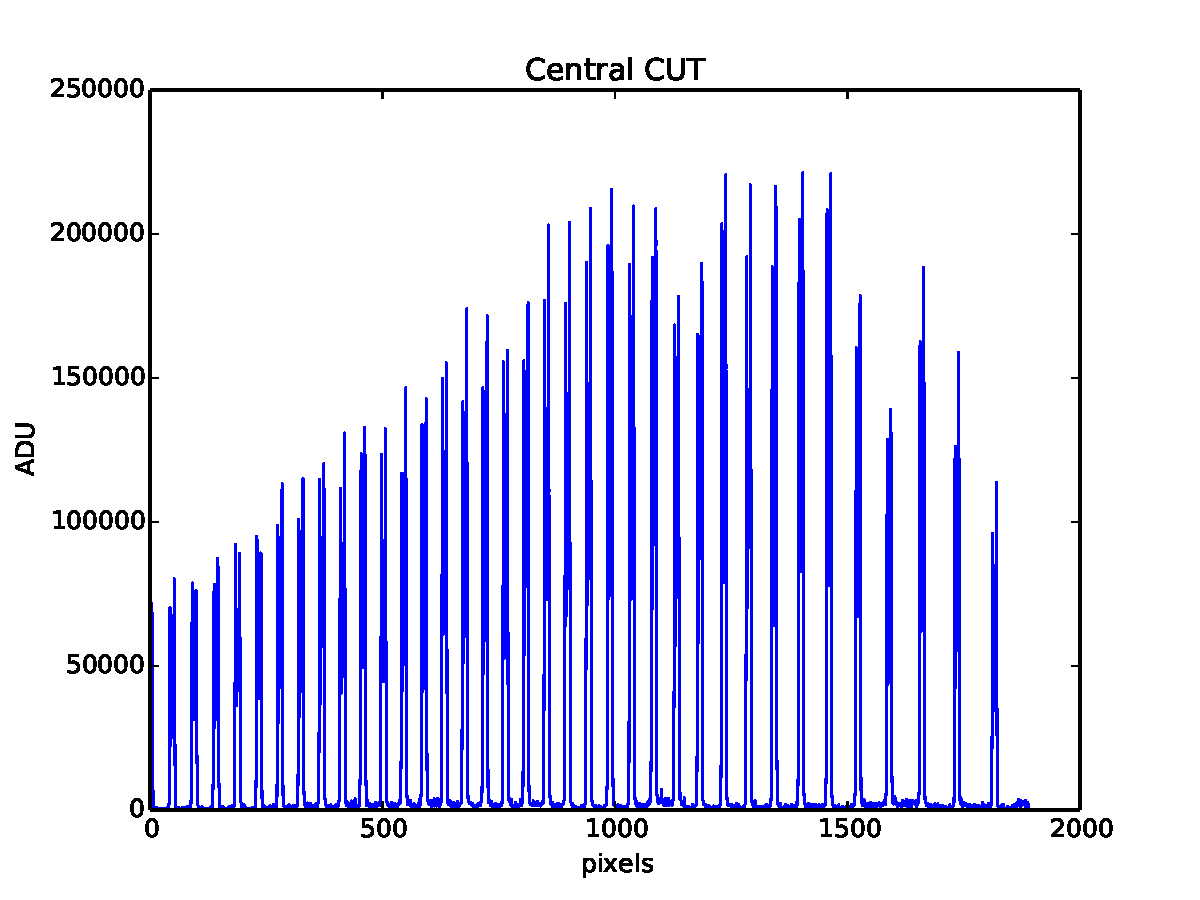
\includegraphics[width=.8\textwidth]{figures/cal_loc_RAW_spirou_1.pdf}
\caption{Pixel number (across order) against flux value of central pixel. \label{figure:cal_loc_RAW_spirou_1}}
\end{center}
\end{figure}

\begin{figure}
\begin{center}
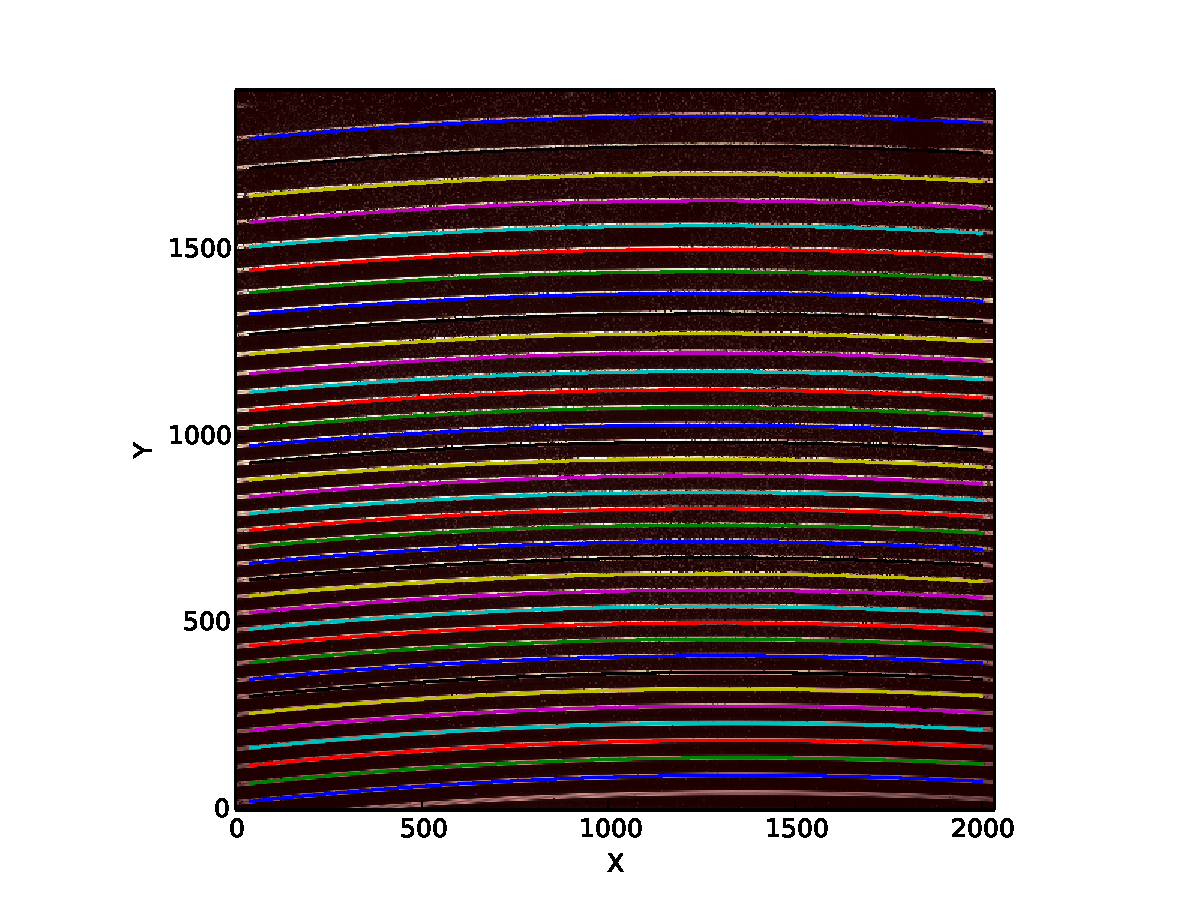
\includegraphics[width=.8\textwidth]{figures/cal_loc_RAW_spirou_2.pdf}
\caption{Image with fits to each order. \label{figure:cal_loc_RAW_spirou_2}}
\end{center}
\end{figure}

% ----------------------------------------------------------------------------------
\clearpage
\newpage
\section{The cal\_SLIT\_spirou recipe}
\label{section:cal_SLIT_spirou}
% ----------------------------------------------------------------------------------

Fabry-Perot exposures in which the three fibres are simultaneously fed by light from the Fabry-Perot filter. Each exposure is used to build the slit orientation. Finds the tilt of the orders. \\

% \TODO{Once writen up the new version update this description}

\noindent File prefixes allowed:
\begin{itemize}
	\item fp\_fp
\end{itemize}


\subsection{Summary of procedure}
\begin{enumerate}
\item adds all fp\_fp files together
\item corrects for dark
\item resizes the image
\item extracts the orders (no weight no tilt)
\item works out the tilt for each order using the location and width
\item saves the tilt to file
\item should do some quality control
\item  updates calibDB with key ``TILT''
\end{enumerate}

\subsection{Running cal\_}
To run cal\_ type:
\begin{lstlisting}[language=bash, style=bashstyle]
cal_SLIT_spirou.p  night_repository  filenames
\end{lstlisting}

\noindent Note: filesnames must start with `fp\_fp'

\subsection{Example working run}

An example run where everything worked is below:

\begin{lstlisting}[style=text]
cal_SLIT_spirou.py 20170710 fp_fp02a203.fits fp_fp03a203.fits fp_fp04a203.fits

||DRS  SPIROU   v   (interactive mode)
16:26:55.3 -   || *****************************************
16:26:55.3 -   || * SPIROU \@(#) Geneva Observatory ()
16:26:55.3 -   || *****************************************
16:26:55.3 -   ||(dir_data_raw)      DRS_DATA_RAW=/scratch/Projects/SPIRou_Pipeline/data/raw/
16:26:55.3 -   ||(dir_data_reduc)    DRS_DATA_REDUC=/scratch/Projects/SPIRou_Pipeline/data/reduced/
16:26:55.3 -   ||(dir_drs_config)    DRS_CONFIG=/scratch/Projects/SPIRou_Pipeline/INTROOT/DRS_SPIROU/config/
16:26:55.3 -   ||(dir_calib_db)      DRS_CALIB_DB=/scratch/Projects/SPIRou_Pipeline/data/calibDB
16:26:55.3 -   ||(dir_data_msg)      DRS_DATA_MSG=/scratch/Projects/SPIRou_Pipeline/data/msg/
16:26:55.3 -   ||(print_log)         DRS_LOG=1         %(0: minimum stdin-out logs)
16:26:55.3 -   ||(plot_graph)        DRS_PLOT=NONE            %(def/undef/trigger)
16:26:55.3 -   ||(used_date)         DRS_USED_DATE=undefined
16:26:55.3 -   ||(working_dir)       DRS_DATA_WORKING=/scratch/Projects/SPIRou_Pipeline/data/tmp/
16:26:55.3 -   ||                    DRS_INTERACTIVE is  set
16:26:55.3 -   |-c:+[...]|Now running : -c on file(s):  fp_fp02a203.fits fp_fp03a203.fits fp_fp04a203.fits
16:26:55.3 -   |-c:+[...]|On directory /scratch/Projects/SPIRou_Pipeline/data/raw/20170710
16:26:55.3 -   |-c:+[...]|ICDP loaded from: /scratch/Projects/SPIRou_Pipeline/INTROOT/DRS_SPIROU/config/hadmrICDP_SPIROU.py
16:26:55.4 -   |-c:+[...]|Calibration file: fp_fp02a203_tilt.fits already exists - not copied
16:26:55.4 -   |-c:+[...]|Calibration file: dark_flat02f10_loco_C.fits already exists - not copied
16:26:55.4 -   |-c:+[...]|Calibration file: dark_flat02f10_order_profil_C.fits already exists - not copied
16:26:55.5 -   |-c:+[...]|Calibration file: flat_dark02f10_order_profil_AB.fits already exists - not copied
16:26:55.5 -   |-c:+[...]|Calibration file: spirou_wave_ini3.fits already exists - not copied
16:26:55.5 -   |-c:+[...]|Calibration file: dark_dark02d406.fits already exists - not copied
16:26:55.5 -   |-c:+[...]|Calibration file: dark_flat02f10_flat_C.fits already exists - not copied
16:26:55.5 -   |-c:+[...]|Calibration file: flat_dark02f10_loco_AB.fits already exists - not copied
16:26:55.5 -   |-c:+[...]|Reading File: /scratch/Projects/SPIRou_Pipeline/data/raw/20170710/fp_fp02a203.fits
16:26:55.5 -   |-c:+[...]|Image 2048x2048 loaded
16:26:55.6 - * |-c:+[...]|Adding frames
16:26:55.6 -   |-c:+[...]|Reading File: /scratch/Projects/SPIRou_Pipeline/data/raw/20170710/fp_fp03a203.fits
16:26:55.6 -   |-c:+[...]|Reading File: /scratch/Projects/SPIRou_Pipeline/data/raw/20170710/fp_fp04a203.fits
16:26:55.9 -   |-c:+[...]|Doing Dark Correction using /scratch/Projects/SPIRou_Pipeline/data/calibDB/dark_dark02d406.fits
16:26:56.2 -   |-c:+[...]|Image format changed to 2035x1930
16:26:56.7 - * |-c:+[...]|Nb pixels morts = 611716 / 15.58 %
16:26:56.7 -   |-c:+[...]|Reading localization parameters of Fiber AB
16:26:57.0 -   |-c:+[...]|Order  0 : Tilt = 4.70 pixel sur 37.0 = -7.24 deg
16:26:57.2 -   |-c:+[...]|Order  1 : Tilt = 4.60 pixel sur 37.4 = -7.02 deg
16:26:57.4 -   |-c:+[...]|Order  2 : Tilt = 4.50 pixel sur 36.8 = -6.97 deg
16:26:57.6 -   |-c:+[...]|Order  3 : Tilt = 4.30 pixel sur 36.4 = -6.74 deg
16:26:57.8 -   |-c:+[...]|Order  4 : Tilt = 4.20 pixel sur 36.8 = -6.52 deg
16:26:58.0 -   |-c:+[...]|Order  5 : Tilt = 4.20 pixel sur 36.0 = -6.65 deg
16:26:58.2 -   |-c:+[...]|Order  6 : Tilt = 4.00 pixel sur 36.1 = -6.33 deg
16:26:58.4 -   |-c:+[...]|Order  7 : Tilt = 4.00 pixel sur 35.7 = -6.40 deg
16:26:58.6 -   |-c:+[...]|Order  8 : Tilt = 3.90 pixel sur 36.7 = -6.07 deg
16:26:58.8 -   |-c:+[...]|Order  9 : Tilt = 3.80 pixel sur 36.1 = -6.01 deg
16:26:59.0 -   |-c:+[...]|Order 10 : Tilt = 3.60 pixel sur 35.7 = -5.76 deg
16:26:59.3 -   |-c:+[...]|Order 11 : Tilt = 3.60 pixel sur 35.7 = -5.75 deg
16:26:59.5 -   |-c:+[...]|Order 12 : Tilt = 3.50 pixel sur 35.9 = -5.57 deg
16:26:59.7 -   |-c:+[...]|Order 13 : Tilt = 3.30 pixel sur 35.8 = -5.27 deg
16:26:59.8 -   |-c:+[...]|Order 14 : Tilt = 3.30 pixel sur 35.9 = -5.25 deg
16:27:00.0 -   |-c:+[...]|Order 15 : Tilt = 3.20 pixel sur 35.4 = -5.17 deg
16:27:00.2 -   |-c:+[...]|Order 16 : Tilt = 3.10 pixel sur 35.5 = -4.99 deg
16:27:00.3 -   |-c:+[...]|Order 17 : Tilt = 3.00 pixel sur 35.4 = -4.85 deg
16:27:00.5 -   |-c:+[...]|Order 18 : Tilt = 2.90 pixel sur 35.1 = -4.73 deg
16:27:00.7 -   |-c:+[...]|Order 19 : Tilt = 2.80 pixel sur 35.1 = -4.57 deg
16:27:00.8 -   |-c:+[...]|Order 20 : Tilt = 2.70 pixel sur 34.9 = -4.42 deg
16:27:01.0 -   |-c:+[...]|Order 21 : Tilt = 2.60 pixel sur 34.6 = -4.29 deg
16:27:01.2 -   |-c:+[...]|Order 22 : Tilt = 2.50 pixel sur 34.9 = -4.09 deg
16:27:01.3 -   |-c:+[...]|Order 23 : Tilt = 2.40 pixel sur 34.2 = -4.01 deg
16:27:01.5 -   |-c:+[...]|Order 24 : Tilt = 2.30 pixel sur 34.9 = -3.77 deg
16:27:01.7 -   |-c:+[...]|Order 25 : Tilt = 2.20 pixel sur 34.7 = -3.63 deg
16:27:01.8 -   |-c:+[...]|Order 26 : Tilt = 2.00 pixel sur 34.2 = -3.35 deg
16:27:02.0 -   |-c:+[...]|Order 27 : Tilt = 2.00 pixel sur 34.5 = -3.32 deg
16:27:02.2 -   |-c:+[...]|Order 28 : Tilt = 1.80 pixel sur 34.2 = -3.01 deg
16:27:02.3 -   |-c:+[...]|Order 29 : Tilt = 1.70 pixel sur 34.0 = -2.86 deg
16:27:02.5 -   |-c:+[...]|Order 30 : Tilt = 1.60 pixel sur 33.6 = -2.73 deg
16:27:02.7 -   |-c:+[...]|Order 31 : Tilt = 1.40 pixel sur 34.0 = -2.36 deg
16:27:02.8 -   |-c:+[...]|Order 32 : Tilt = 1.40 pixel sur 33.5 = -2.40 deg
16:27:03.0 -   |-c:+[...]|Order 33 : Tilt = 1.10 pixel sur 32.4 = -1.94 deg
16:27:03.2 -   |-c:+[...]|Order 34 : Tilt = 1.00 pixel sur 32.1 = -1.79 deg
16:27:03.3 -   |-c:+[...]|Order 35 : Tilt = 0.90 pixel sur 33.7 = -1.53 deg
16:27:03.3 - * |-c:+[...]AB|Tilt dispersion = 0.069 deg
16:27:03.6 -   |-c:+[...]|Saving tilt information in file: fp_fp02a203_tilt.fits
16:27:05.2 - * |-c:+[...]|Updating Calib Data Base with TILT
16:27:05.2 - * |-c:+[...]|Recipe -c has been successfully completed
\end{lstlisting}

\subsection{Interactive mode}

\begin{figure}
\begin{center}
\vcenteredhbox{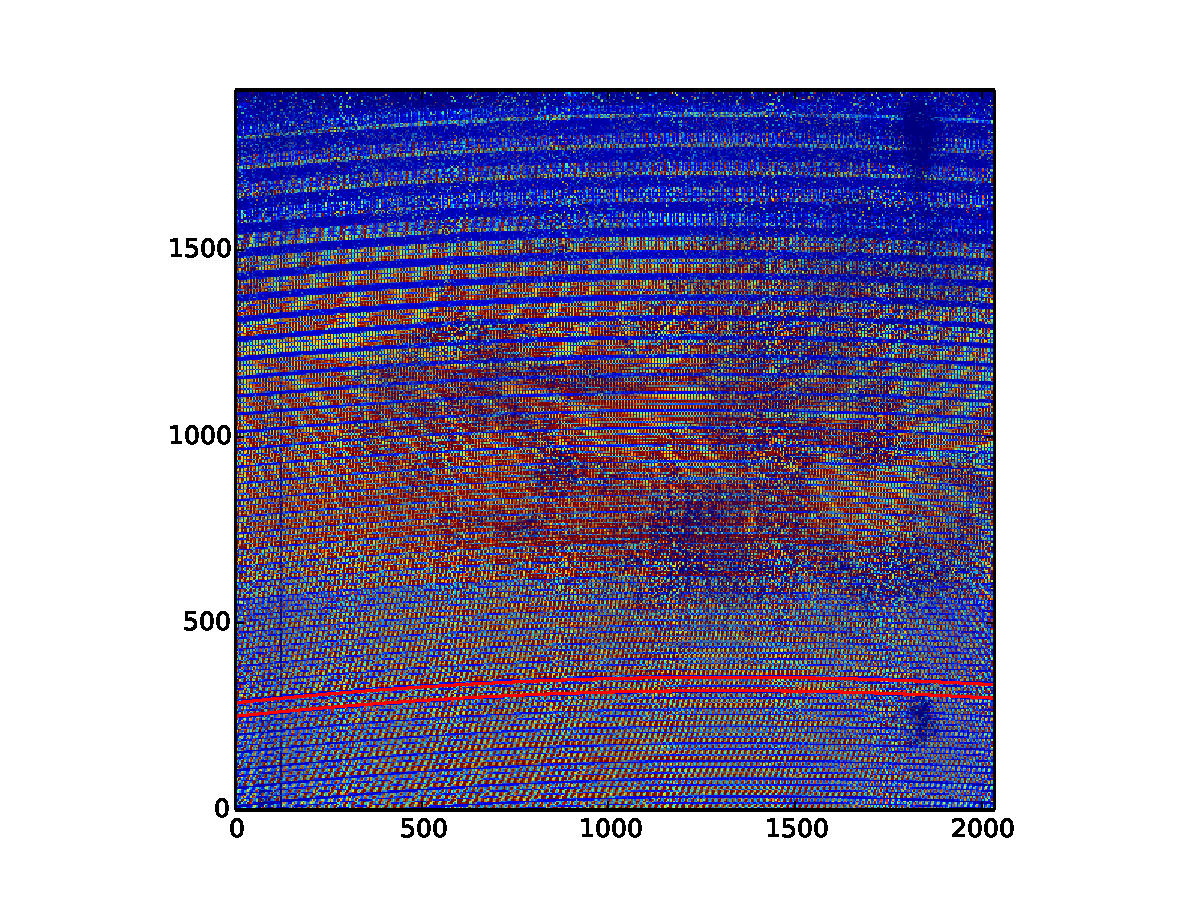
\includegraphics[width=.49\textwidth]{figures/cal_SLIT_spirou_1.pdf}}
\vcenteredhbox{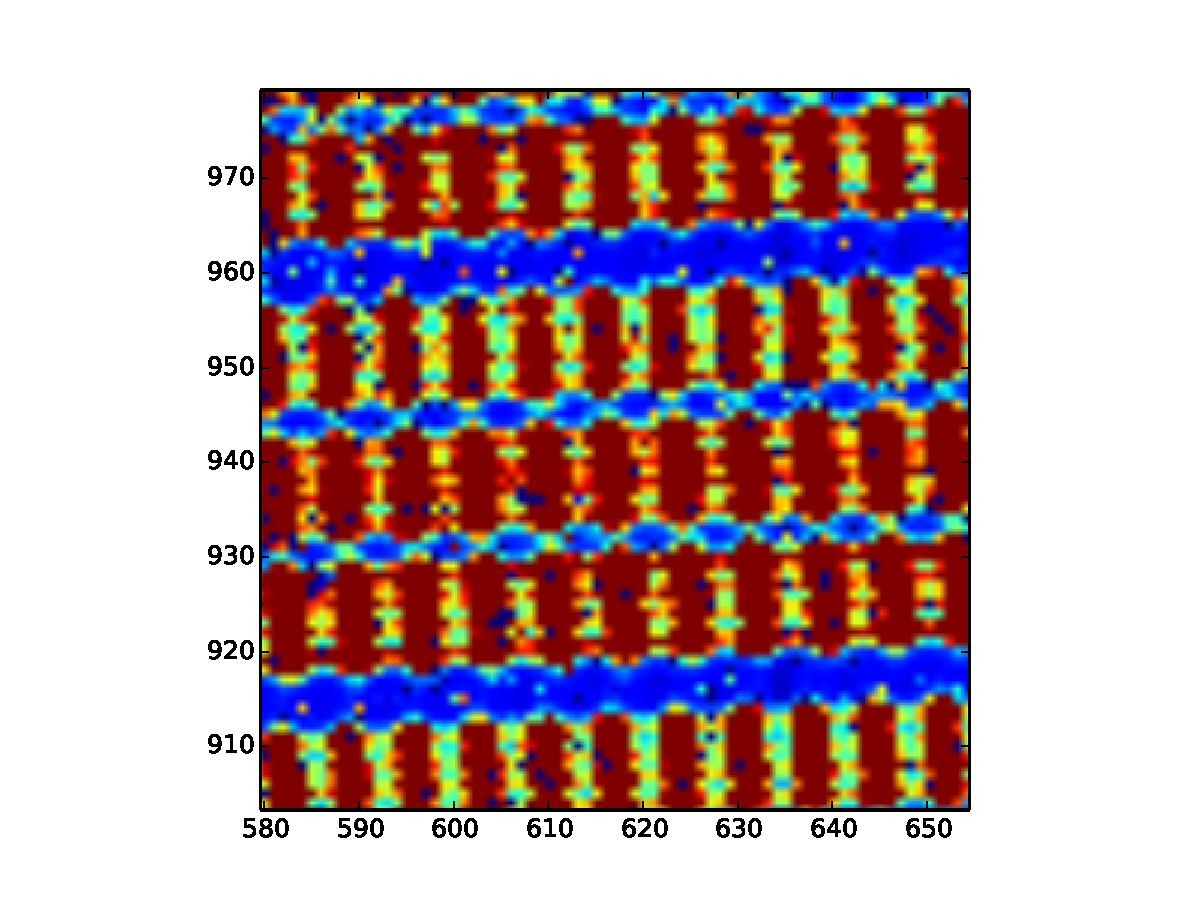
\includegraphics[width=.49\textwidth]{figures/cal_SLIT_spirou_1a.pdf}}
\caption{Left: The full `fp\_fp' image. Right: Zoom in on a section of the `fp\_fp' image showing the tilt.\label{figure:cal_slit_spirou_1}}
\end{center}
\end{figure}

\begin{figure}
\begin{center}
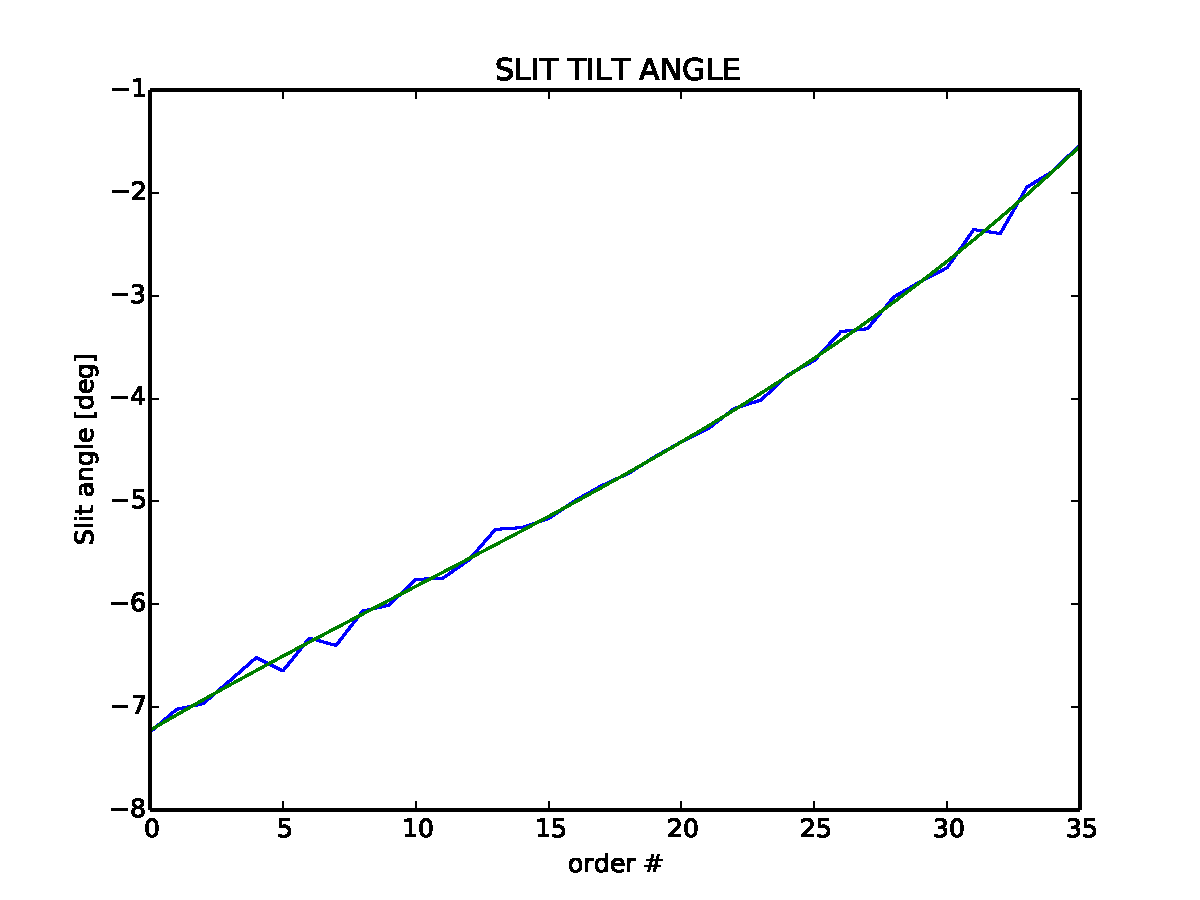
\includegraphics[width=.8\textwidth]{figures/cal_SLIT_spirou_2.pdf}
\caption{Slit aginle as a function of order number. \label{figure:cal_slit_spirou_2}}
\end{center}
\end{figure}

% ----------------------------------------------------------------------------------
\clearpage
\newpage
\section{The cal\_FF\_RAW\_spirou recipe}
\label{section:cal_FF_RAW_spirou}
% ----------------------------------------------------------------------------------

Creates the flat fields. \\ 

% \TODO{Once writen up the new version update this description} \\

\noindent File prefixes allowed:
\begin{itemize}
	\item dark\_flat
	\item flat\_dark
\end{itemize}

\noindent \textcolor{red}{Note: if using same files in Section \ref{section:working_example} you will get an error message when running the file}.
\noindent To solve this open the `master\_calib\_SPIROU.txt' file located in \textcolor{blue}{\{DATA\_ROOT\_CALIB\}}. Edit the unix date in the line that begins `TILT' so that it is less than the unix date on rwos `ORDER\_PROFIL\_AB' (i.e. change it from 1499707515.0 to 1499705515.0).

\noindent i.e. the `master\_calib\_SPIROU.txt' file should look go from
\begin{lstlisting}[style=text]
DARK 20170710 dark_dark02d406.fits 07/10/17/16:37:48 1499704668.0
ORDER_PROFIL_C 20170710 dark_flat02f10_order_profil_C.fits 07/10/17/17:03:50 1499706230.0
LOC_C 20170710 dark_flat02f10_loco_C.fits 07/10/17/17:03:50 1499706230.0
ORDER_PROFIL_AB 20170710 flat_dark02f10_order_profil_AB.fits 07/10/17/17:07:08 1499706428.0
LOC_AB 20170710 flat_dark02f10_loco_AB.fits 07/10/17/17:07:08 1499706428.0
TILT 20170710 fp_fp02a203_tilt.fits 07/10/17/17:25:15 @1499707515.0@
\end{lstlisting}

\noindent to this:

\definecolor{shadecolor}{named}{Tan} 
\begin{lstlisting}[style=text]
DARK 20170710 dark_dark02d406.fits 07/10/17/16:37:48 1499704668.0
ORDER_PROFIL_C 20170710 dark_flat02f10_order_profil_C.fits 07/10/17/17:03:50 1499706230.0
LOC_C 20170710 dark_flat02f10_loco_C.fits 07/10/17/17:03:50 1499706230.0
ORDER_PROFIL_AB 20170710 flat_dark02f10_order_profil_AB.fits 07/10/17/17:07:08 1499706428.0
LOC_AB 20170710 flat_dark02f10_loco_AB.fits 07/10/17/17:07:08 1499706428.0
TILT 20170710 fp_fp02a203_tilt.fits 07/10/17/17:25:15 @1499705515.0@

\end{lstlisting}

\subsection{Summary of procedure}
\begin{enumerate}
\item adds all `dark\_flat' or `flat\_dark' files together
\item corrects for darks
\item resizes the image
\item possible background subtraction?
\item extracts the orders using tilt and weight
\item calculates the blaze
\item calculates the flat field, (flat = extraction / blaze)
\item stores the flat fields
\item does some quality control
\item updates calibDB with key "FLAT\_\definekeyword{fiber}" where \definekeyword{fiber} = [AB, C] etc
\end{enumerate}

\subsection{Running cal\_FF\_RAW\_spirou}

To run cal\_FF\_RAW\_spirou type:
\begin{lstlisting}[language=bash, style=bashstyle]
cal_FF_RAW_spirou.py  night_repository  filenames
\end{lstlisting}

\noindent Note: filenames must start with `dark\_flat' or `flat\_dark'

\subsection{Example working run}

An example run where everything worked is below:

\begin{lstlisting}[style=text]
cal_FF_RAW_spirou.py 20170710 dark_flat02f10.fits dark_flat03f10.fits
dark_flat04f10.fits dark_flat05f10.fits dark_flat06f10.fits

||DRS  SPIROU   v   (interactive mode)
16:49:40.5 -   || *****************************************
16:49:40.5 -   || * SPIROU \@(#) Geneva Observatory ()
16:49:40.5 -   || *****************************************
16:49:40.5 -   ||(dir_data_raw)      DRS_DATA_RAW=/scratch/Projects/SPIRou_Pipeline/data/raw/
16:49:40.5 -   ||(dir_data_reduc)    DRS_DATA_REDUC=/scratch/Projects/SPIRou_Pipeline/data/reduced/
16:49:40.5 -   ||(dir_drs_config)    DRS_CONFIG=/scratch/Projects/SPIRou_Pipeline/INTROOT/DRS_SPIROU/config/
16:49:40.5 -   ||(dir_calib_db)      DRS_CALIB_DB=/scratch/Projects/SPIRou_Pipeline/data/calibDB
16:49:40.5 -   ||(dir_data_msg)      DRS_DATA_MSG=/scratch/Projects/SPIRou_Pipeline/data/msg/
16:49:40.5 -   ||(print_log)         DRS_LOG=1         %(0: minimum stdin-out logs)
16:49:40.5 -   ||(plot_graph)        DRS_PLOT=NONE            %(def/undef/trigger)
16:49:40.5 -   ||(used_date)         DRS_USED_DATE=undefined
16:49:40.5 -   ||(working_dir)       DRS_DATA_WORKING=/scratch/Projects/SPIRou_Pipeline/data/tmp/
16:49:40.5 -   ||                    DRS_INTERACTIVE is  set
16:49:40.5 -   |-c:+[...]|Now running : -c on file(s):  dark_flat02f10.fits dark_flat03f10.fits
16:49:40.5 -   |-c:+[...]|On directory /scratch/Projects/SPIRou_Pipeline/data/raw/20170710
16:49:40.5 -   |-c:+[...]|ICDP loaded from: /scratch/Projects/SPIRou_Pipeline/INTROOT/DRS_SPIROU/config/hadmrICDP_SPIROU.py
16:49:40.5 - * |-c:+[...]|Now processing Image TYPE: UNKNOWN  with -c recipe
16:49:40.6 -   |-c:+[...]|Calibration file: dark_dark02d406.fits already exists - not copied
16:49:40.6 -   |-c:+[...]|Calibration file: fp_fp02a203_tilt.fits already exists - not copied
16:49:40.6 -   |-c:+[...]|Reading File: /scratch/Projects/SPIRou_Pipeline/data/raw/20170710/dark_flat02f10.fits
16:49:40.6 -   |-c:+[...]|Image 2048x2048 loaded
16:49:40.6 - * |-c:+[...]|Adding frames
16:49:40.6 -   |-c:+[...]|Reading File: /scratch/Projects/SPIRou_Pipeline/data/raw/20170710/dark_flat03f10.fits
16:49:40.7 -   |-c:+[...]|Doing Dark Correction using /scratch/Projects/SPIRou_Pipeline/data/calibDB/dark_dark02d406.fits
16:49:41.0 -   |-c:+[...]|Image format changed to 2035x1930
16:49:41.5 - * |-c:+[...]|Nb pixels morts = 568533 / 14.48 %
16:49:41.5 - * |-c:+[...]|Maximum average flux/pixel in the spectrum: 73264.1[ADU]
16:49:41.5 -   |-c:+[...]|Reading tilt slit 
16:49:41.5 -   |-c:+[...]C|Reading localization parameters of Fiber C
16:49:41.6 -   |-c:+[...]C|Reading order profil of Fiber C
16:49:42.1 -   |-c:+[...]|On fiber C  order  0: S/N= 685.6  - FF rms= 4.68 %
16:49:42.7 -   |-c:+[...]|On fiber C  order  1: S/N= 709.3  - FF rms= 4.81 %
16:49:43.3 -   |-c:+[...]|On fiber C  order  2: S/N= 733.7  - FF rms= 4.75 %
16:49:43.8 -   |-c:+[...]|On fiber C  order  3: S/N= 759.2  - FF rms= 4.86 %
16:49:44.4 -   |-c:+[...]|On fiber C  order  4: S/N= 780.7  - FF rms= 4.94 %
16:49:44.9 -   |-c:+[...]|On fiber C  order  5: S/N= 811.4  - FF rms= 5.03 %
16:49:45.5 -   |-c:+[...]|On fiber C  order  6: S/N= 842.1  - FF rms= 5.11 %
16:49:46.0 -   |-c:+[...]|On fiber C  order  7: S/N= 875.4  - FF rms= 5.23 %
16:49:46.6 -   |-c:+[...]|On fiber C  order  8: S/N= 893.9  - FF rms= 5.37 %
16:49:47.2 -   |-c:+[...]|On fiber C  order  9: S/N= 916.4  - FF rms= 6.07 %
16:49:47.7 -   |-c:+[...]|On fiber C  order 10: S/N= 928.3  - FF rms= 8.02 %
16:49:48.3 -   |-c:+[...]|On fiber C  order 11: S/N= 912.5  - FF rms= 6.84 %
16:49:48.8 -   |-c:+[...]|On fiber C  order 12: S/N= 961.8  - FF rms= 5.94 %
16:49:49.4 -   |-c:+[...]|On fiber C  order 13: S/N= 1004.9  - FF rms= 5.97 %
16:49:49.9 -   |-c:+[...]|On fiber C  order 14: S/N= 1022.5  - FF rms= 6.15 %
16:49:50.5 -   |-c:+[...]|On fiber C  order 15: S/N= 1045.5  - FF rms= 6.18 %
16:49:51.1 -   |-c:+[...]|On fiber C  order 16: S/N= 1053.4  - FF rms= 6.14 %
16:49:51.6 -   |-c:+[...]|On fiber C  order 17: S/N= 1085.8  - FF rms= 6.23 %
16:49:52.2 -   |-c:+[...]|On fiber C  order 18: S/N= 1103.0  - FF rms= 6.28 %
16:49:52.7 -   |-c:+[...]|On fiber C  order 19: S/N= 1134.8  - FF rms= 6.77 %
16:49:53.3 -   |-c:+[...]|On fiber C  order 20: S/N= 1150.4  - FF rms= 6.43 %
16:49:53.9 -   |-c:+[...]|On fiber C  order 21: S/N= 1144.2  - FF rms= 6.42 %
16:49:54.4 -   |-c:+[...]|On fiber C  order 22: S/N= 1139.6  - FF rms= 6.39 %
16:49:55.0 -   |-c:+[...]|On fiber C  order 23: S/N= 1161.3  - FF rms= 6.52 %
16:49:55.5 -   |-c:+[...]|On fiber C  order 24: S/N= 1137.8  - FF rms= 9.11 %
16:49:56.1 -   |-c:+[...]|On fiber C  order 25: S/N= 1131.4  - FF rms= 9.39 %
16:49:56.6 -   |-c:+[...]|On fiber C  order 26: S/N= 1113.7  - FF rms= 7.97 %
16:49:57.2 -   |-c:+[...]|On fiber C  order 27: S/N= 1161.7  - FF rms= 6.04 %
16:49:57.7 -   |-c:+[...]|On fiber C  order 28: S/N= 1153.9  - FF rms= 6.07 %
16:49:58.3 -   |-c:+[...]|On fiber C  order 29: S/N= 1178.2  - FF rms= 5.89 %
16:49:58.9 -   |-c:+[...]|On fiber C  order 30: S/N= 1150.4  - FF rms= 5.92 %
16:49:59.6 -   |-c:+[...]|On fiber C  order 31: S/N= 1024.1  - FF rms= 5.60 %
16:50:00.3 -   |-c:+[...]|On fiber C  order 32: S/N= 945.1  - FF rms= 5.60 %
16:50:01.0 -   |-c:+[...]|On fiber C  order 33: S/N= 1030.4  - FF rms= 5.70 %
16:50:01.6 -   |-c:+[...]|On fiber C  order 34: S/N= 957.7  - FF rms= 8.21 %
16:50:02.2 -   |-c:+[...]|On fiber C  order 35: S/N= 753.1  - FF rms= 8.11 %
16:50:02.4 -   |-c:+[...]C|Saving blaze spectrum for fiber: C in dark_flat02f10_blaze_C.fits
16:50:03.1 -   |-c:+[...]C|Saving FF  spectrum of Fiber C in dark_flat02f10_flat_C.fits
16:50:04.2 - * |-c:+[...]|Updating Calib Data Base with FLAT_C
16:50:04.2 - * |-c:+[...]|Recipe -c has been  successfully completed
\end{lstlisting}

\subsection{Interactive mode}

\begin{figure}
\begin{center}
\vcenteredhbox{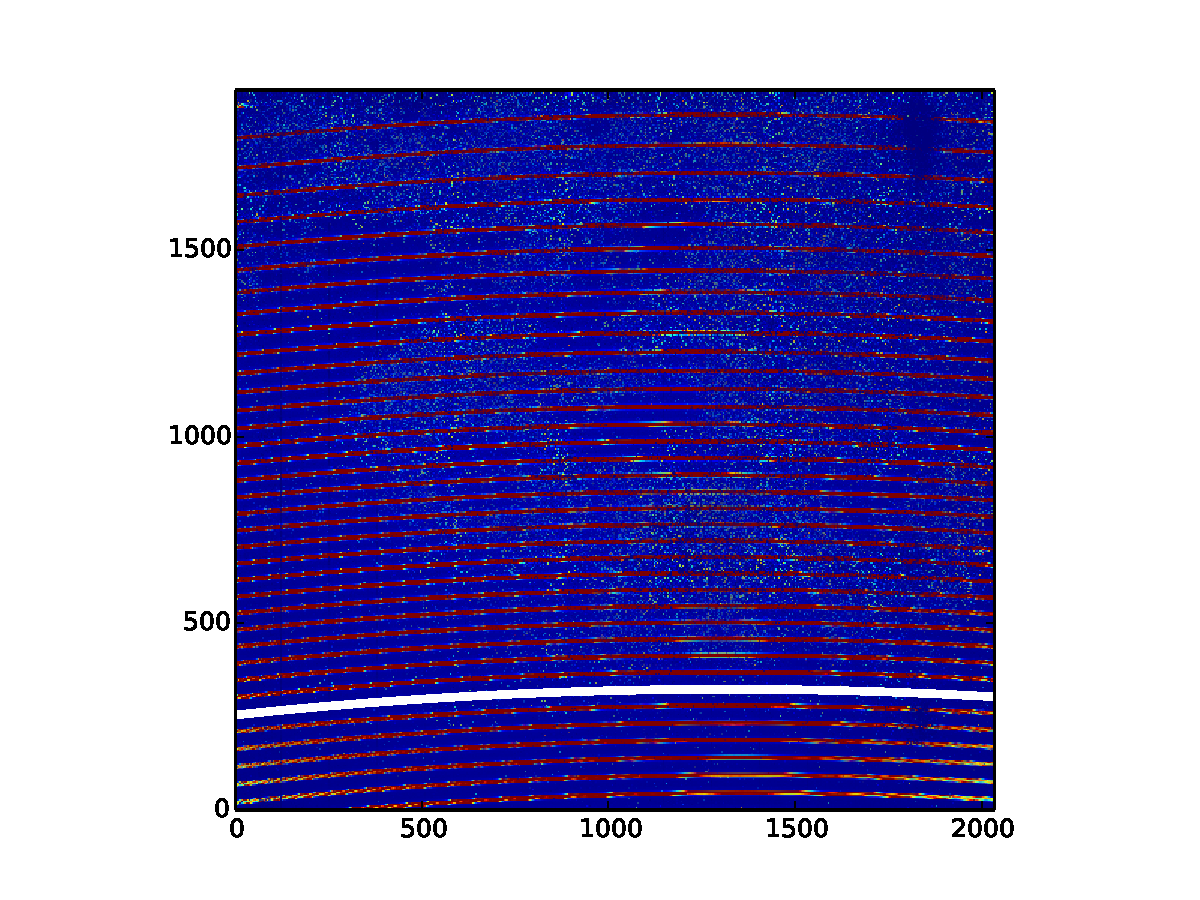
\includegraphics[width=.49\textwidth]{figures/cal_FF_RAW_spirou_1.pdf}}
\vcenteredhbox{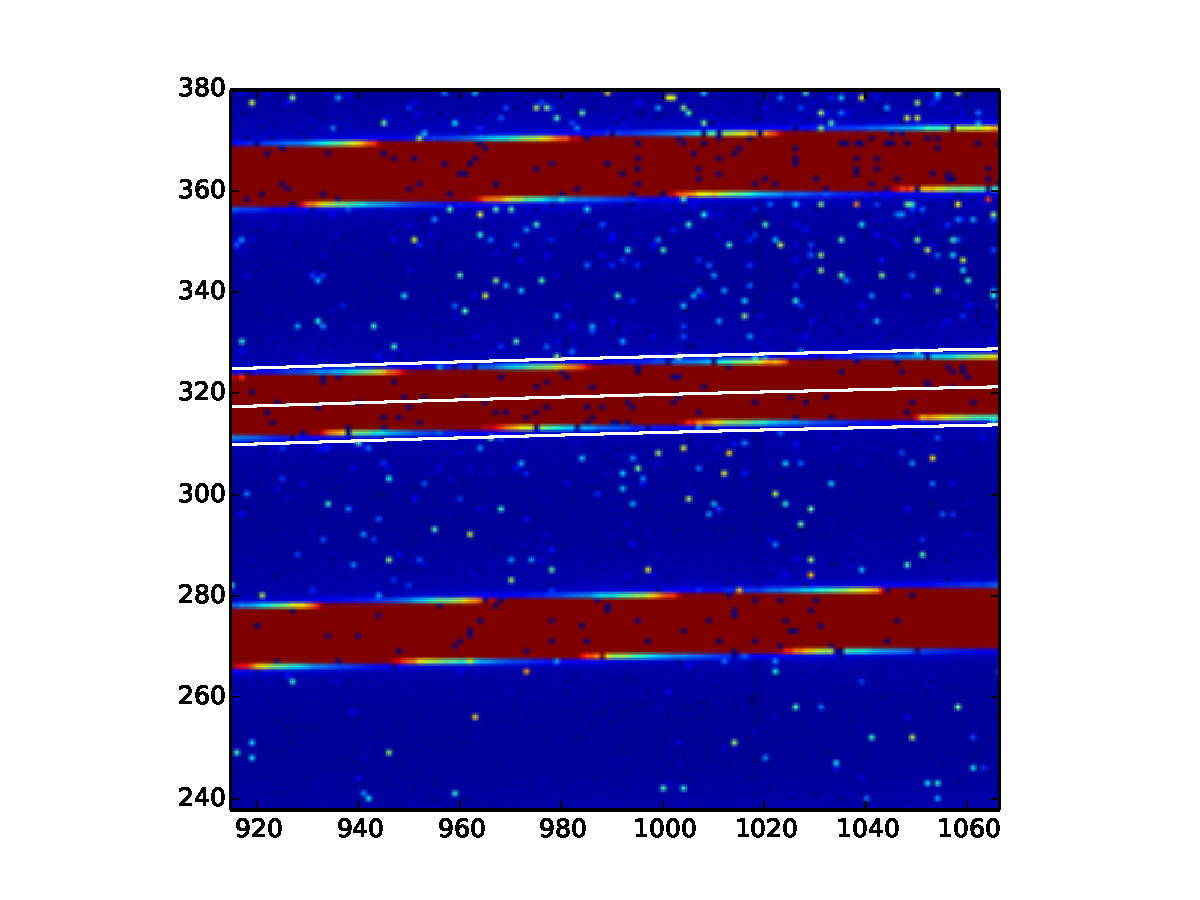
\includegraphics[width=.49\textwidth]{figures/cal_FF_RAW_spirou_1a.pdf}}
\caption{Left: the full processed image with one order fit highlighted. Right: Zoom in of the highlighted order fit. \label{figure:cal_FF_RAW_spirou_1}}
\end{center}
\end{figure}

\begin{figure}
\begin{center}
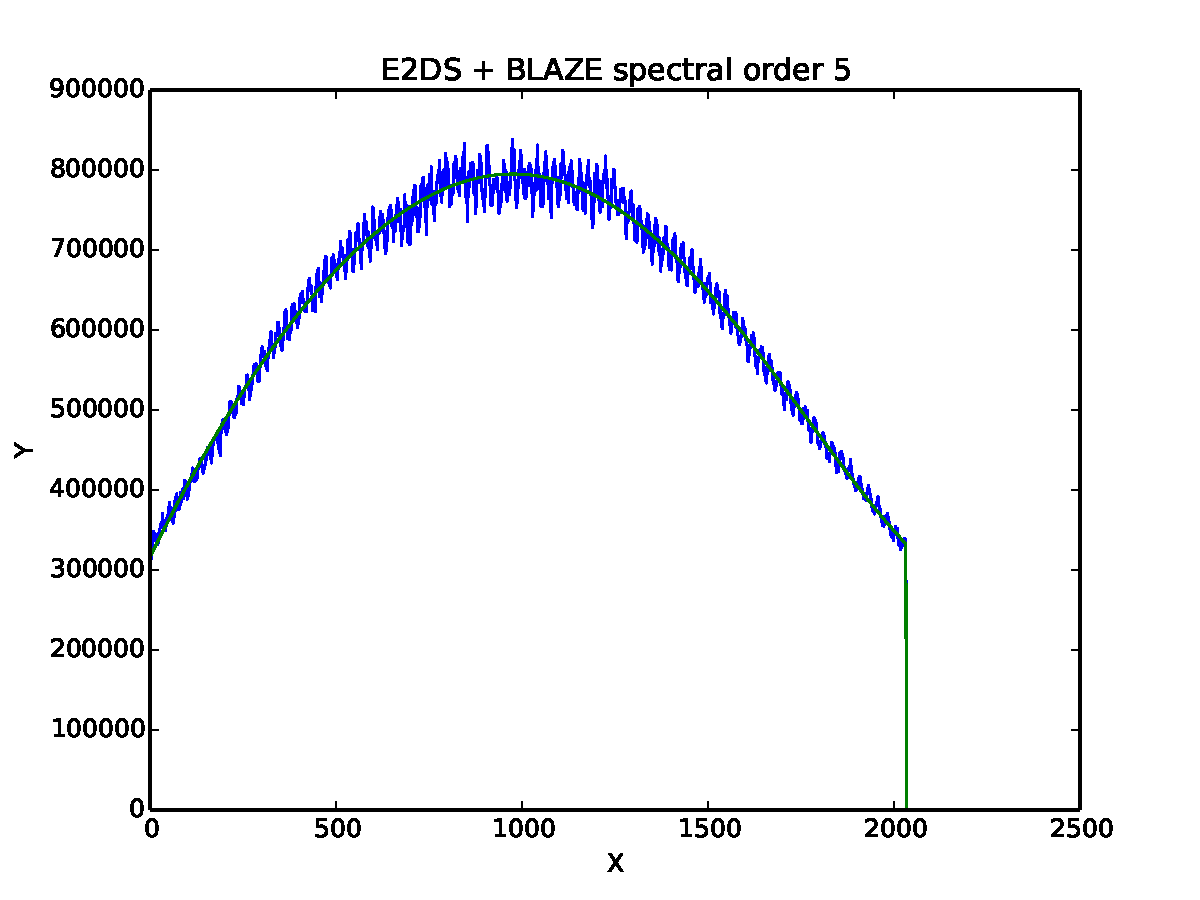
\includegraphics[width=.8\textwidth]{figures/cal_FF_RAW_spirou_2.pdf}
\caption{The extracted highlighted order from Figure \protect\ref{figure:cal_FF_RAW_spirou_1}. Overplotted is the blaze fit (in cyan). \label{figure:cal_FF_RAW_spirou_2}}
\end{center}
\end{figure}

\begin{figure}
\begin{center}
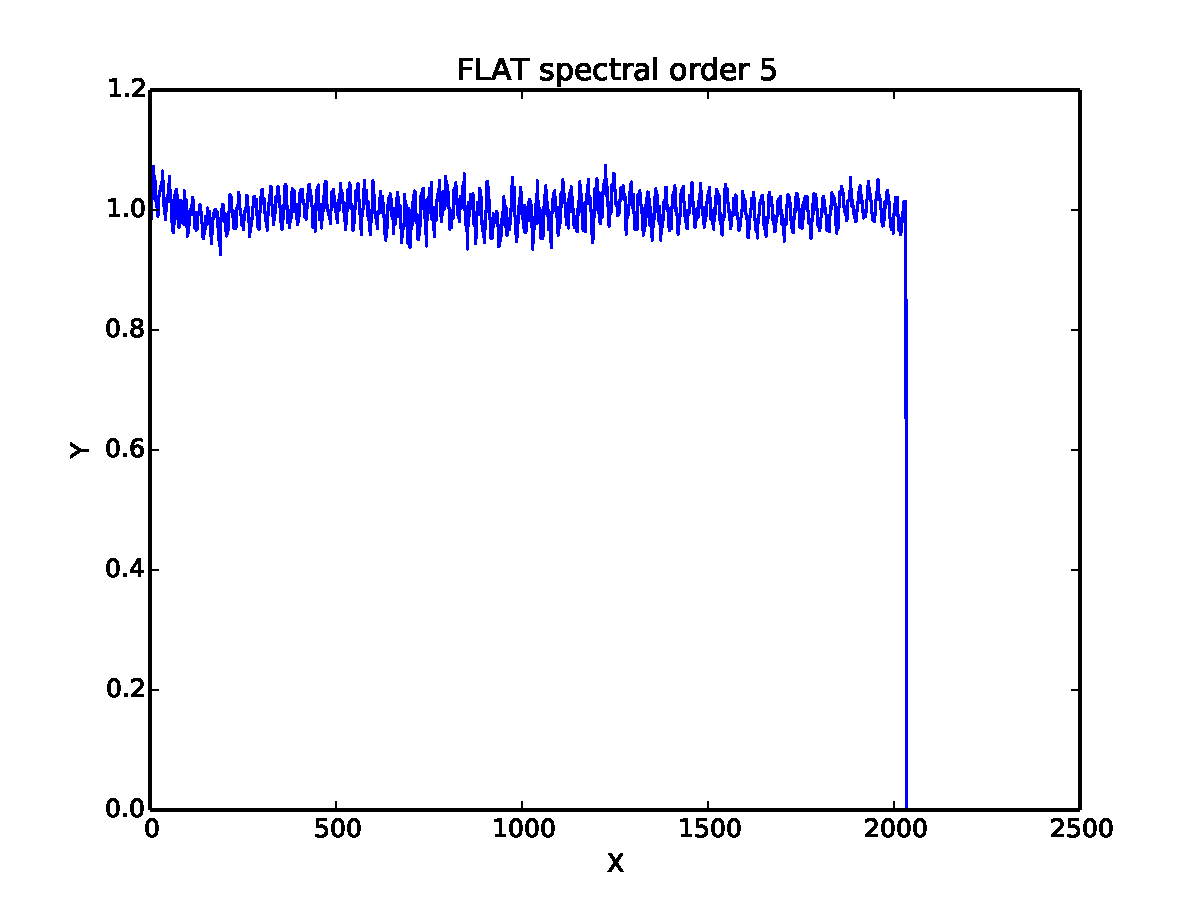
\includegraphics[width=.8\textwidth]{figures/cal_FF_RAW_spirou_3.pdf}
\caption{The flattened order for highlighted order from Figure \protect\ref{figure:cal_FF_RAW_spirou_1}. \label{figure:cal_FF_RAW_spirou_3}}
\end{center}
\end{figure}

% ----------------------------------------------------------------------------------
\clearpage
\newpage
\section{The cal\_extract\_RAW\_spirou recipe}
\label{section:cal_extract_RAW_spirou}
% ----------------------------------------------------------------------------------

Extracts orders for specific fibers and files. \\

\noindent File prefixes allowed:
\begin{itemize}
	\item fp\_fp
	\item hcone\_dark
	\item dark\_hcone
	\item hcone\_hcone
	\item dark\_dark\_AHC1
	\item dark\_hctwo
	\item hctwo\_hctwo
	\item dark\_dark\_AHC2
\end{itemize}

% \TODO{Once writen up the new version update this description}

\subsection{Summary of procedure}
\begin{enumerate}
\item adds all files together
\item corrects for darks
\item resizes the image
\item checks for saturation
\item possible background subtraction?
\item extracts orders
	\begin{itemize}
		\item without tilt/weight fortran
		\item without tilt/weight python
		\item with tilt (no weight)
		\item with tilt and weight
		\item with weight (no tilt)
	\end{itemize}
\item saves extraction with weight (no tilt) to e2ds file
\end{enumerate}

\subsection{Running cal\_extract\_RAW\_spirou}

To run cal\_extract\_RAW\_spirou on fiber=AB:
\begin{lstlisting}[language=bash, style=bashstyle]
cal_extract_RAW_spirouAB.py  night_repository  filenames
\end{lstlisting}
To run cal\_extract\_RAW\_spirou on fiber=C:
\begin{lstlisting}[language=bash, style=bashstyle]
cal_extract_RAW_spirouC.py  night_repository  filenames
\end{lstlisting}

Note: Filenames must start with `fp\_fp', `hcone\_dark', `dark\_hcone', `hcone\_hcone', `dark\_dark\_AHC1', `dark\_hctwo', `hctwo\_hctwo', or `dark\_dark\_AHC2'.


\subsection{Example working run}

An example run where everything worked is below:

\begin{lstlisting}[style=text]
cal_extract_RAW_spirouC.py 20170710 fp_fp02a203.fits fp_fp03a203.fits
fp_fp04a203.fits

||DRS  SPIROU   v   (interactive mode)
17:38:04.5 -   || *****************************************
17:38:04.5 -   || * SPIROU \@(#) Geneva Observatory ()
17:38:04.5 -   || *****************************************
17:38:04.5 -   ||(dir_data_raw)      DRS_DATA_RAW=/scratch/Projects/SPIRou_Pipeline/data/raw/
17:38:04.5 -   ||(dir_data_reduc)    DRS_DATA_REDUC=/scratch/Projects/SPIRou_Pipeline/data/reduced/
17:38:04.5 -   ||(dir_drs_config)    DRS_CONFIG=/scratch/Projects/SPIRou_Pipeline/INTROOT/DRS_SPIROU/config/
17:38:04.5 -   ||(dir_calib_db)      DRS_CALIB_DB=/scratch/Projects/SPIRou_Pipeline/data/calibDB
17:38:04.5 -   ||(dir_data_msg)      DRS_DATA_MSG=/scratch/Projects/SPIRou_Pipeline/data/msg/
17:38:04.5 -   ||(print_log)         DRS_LOG=1         %(0: minimum stdin-out logs)
17:38:04.5 -   ||(plot_graph)        DRS_PLOT=NONE            %(def/undef/trigger)
17:38:04.5 -   ||(used_date)         DRS_USED_DATE=undefined
17:38:04.5 -   ||(working_dir)       DRS_DATA_WORKING=/scratch/Projects/SPIRou_Pipeline/data/tmp/
17:38:04.5 -   ||                    DRS_INTERACTIVE is  set
17:38:04.5 -   |-c:+[...]|Now running : -c on file(s):  fp_fp02a203.fits fp_fp03a203.fits
17:38:04.5 -   |-c:+[...]|On directory /scratch/Projects/SPIRou_Pipeline/data/raw/20170710
17:38:04.5 -   |-c:+[...]|ICDP loaded from: /scratch/Projects/SPIRou_Pipeline/INTROOT/DRS_SPIROU/config/hadmrICDP_SPIROU.py
17:38:04.5 - * |-c:+[...]|Now processing Image TYPE: UNKNOWN  with -c recipe
17:38:04.6 -   |-c:+[...]|Calibration file: fp_fp02a203_tilt.fits already exists - not copied
17:38:04.6 -   |-c:+[...]|Calibration file: dark_flat02f10_loco_C.fits already exists - not copied
17:38:04.6 -   |-c:+[...]|Calibration file: flat_dark02f10_order_profil_AB.fits already exists - not copied
17:38:04.6 -   |-c:+[...]|Calibration file: spirou_wave_ini3.fits already exists - not copied
17:38:04.7 -   |-c:+[...]|Calibration file: dark_dark02d406.fits already exists - not copied
17:38:04.7 -   |-c:+[...]|Calibration file: dark_flat02f10_flat_C.fits already exists - not copied
17:38:04.7 -   |-c:+[...]|Calibration file: dark_flat02f10_order_profil_C.fits already exists - not copied
17:38:04.7 -   |-c:+[...]|Calibration file: flat_dark02f10_loco_AB.fits already exists - not copied
17:38:04.7 -   |-c:+[...]|Reading File: /scratch/Projects/SPIRou_Pipeline/data/raw/20170710/fp_fp02a203.fits
17:38:04.7 -   |-c:+[...]|Image 2048x2048 loaded
17:38:04.8 - * |-c:+[...]|Adding frames
17:38:04.8 -   |-c:+[...]|Reading File: /scratch/Projects/SPIRou_Pipeline/data/raw/20170710/fp_fp03a203.fits
17:38:04.9 -   |-c:+[...]|Doing Dark Correction using /scratch/Projects/SPIRou_Pipeline/data/calibDB/dark_dark02d406.fits
17:38:05.1 -   |-c:+[...]|Image format changed to 2035x1930
17:38:05.6 - * |-c:+[...]|Nb pixels morts = 568485 / 14.47 %
17:38:05.6 - * |-c:+[...]|Maximum average flux/pixel in the spectrum: 110446.0[ADU]
17:38:05.6 -   |-c:+[...]|Reading tilt slit 
17:38:05.7 -   |-c:+[...]|Reading wavelength solution 
17:38:05.7 -   |-c:+[...]C|Reading localization parameters of Fiber C
17:38:05.7 -   |-c:+[...]C|Reading order profil of Fiber C
17:38:07.1 -   |-c:+[...]|On fiber C  order  0: S/N= 712.0  
17:38:08.9 -   |-c:+[...]|On fiber C  order  1: S/N= 780.2  
17:38:10.3 -   |-c:+[...]|On fiber C  order  2: S/N= 726.0  
17:38:12.0 -   |-c:+[...]|On fiber C  order  3: S/N= 700.3  
17:38:13.5 -   |-c:+[...]|On fiber C  order  4: S/N= 702.3  
17:38:14.9 -   |-c:+[...]|On fiber C  order  5: S/N= 740.0  
17:38:16.3 -   |-c:+[...]|On fiber C  order  6: S/N= 773.4  
17:38:17.7 -   |-c:+[...]|On fiber C  order  7: S/N= 758.5  
17:38:19.2 -   |-c:+[...]|On fiber C  order  8: S/N= 752.0  
17:38:20.7 -   |-c:+[...]|On fiber C  order  9: S/N= 763.0  
17:38:22.1 -   |-c:+[...]|On fiber C  order 10: S/N= 794.5  
17:38:23.5 -   |-c:+[...]|On fiber C  order 11: S/N= 671.5  
17:38:25.2 -   |-c:+[...]|On fiber C  order 12: S/N= 871.4  
17:38:26.7 -   |-c:+[...]|On fiber C  order 13: S/N= 883.0  
17:38:28.4 -   |-c:+[...]|On fiber C  order 14: S/N= 1070.7  
17:38:29.9 -   |-c:+[...]|On fiber C  order 15: S/N= 954.4  
17:38:31.6 -   |-c:+[...]|On fiber C  order 16: S/N= 909.4
17:38:33.3 -   |-c:+[...]|On fiber C  order 17: S/N= 935.8
17:38:34.9 -   |-c:+[...]|On fiber C  order 18: S/N= 905.3
17:38:36.4 -   |-c:+[...]|On fiber C  order 19: S/N= 888.5
17:38:37.8 -   |-c:+[...]|On fiber C  order 20: S/N= 896.3
17:38:39.6 -   |-c:+[...]|On fiber C  order 21: S/N= 888.1
17:38:41.3 -   |-c:+[...]|On fiber C  order 22: S/N= 848.4
17:38:43.0 -   |-c:+[...]|On fiber C  order 23: S/N= 860.3
17:38:44.7 -   |-c:+[...]|On fiber C  order 24: S/N= 817.9
17:38:46.1 -   |-c:+[...]|On fiber C  order 25: S/N= 813.0
17:38:47.5 -   |-c:+[...]|On fiber C  order 26: S/N= 792.2
17:38:49.0 -   |-c:+[...]|On fiber C  order 27: S/N= 836.9
17:38:50.7 -   |-c:+[...]|On fiber C  order 28: S/N= 882.4
17:38:52.3 -   |-c:+[...]|On fiber C  order 29: S/N= 837.6
17:38:53.7 -   |-c:+[...]|On fiber C  order 30: S/N= 785.7
17:38:55.1 -   |-c:+[...]|On fiber C  order 31: S/N= 434.9
17:38:56.5 -   |-c:+[...]|On fiber C  order 32: S/N= 376.3
17:38:58.0 -   |-c:+[...]|On fiber C  order 33: S/N= 614.3
17:38:59.7 -   |-c:+[...]|On fiber C  order 34: S/N= 523.1
17:39:01.2 -   |-c:+[...]|On fiber C  order 35: S/N= 343.2
17:39:01.5 -   |-c:+[...]|Saving E2DS spectrum of Fiber C in fp_fp02a203_e2ds_C.fits
17:39:02.1 - * |-c:+[...]|Recipe -c has been  successfully completed
\end{lstlisting}

\subsection{Interactive mode}

\begin{figure}
\begin{center}
\vcenteredhbox{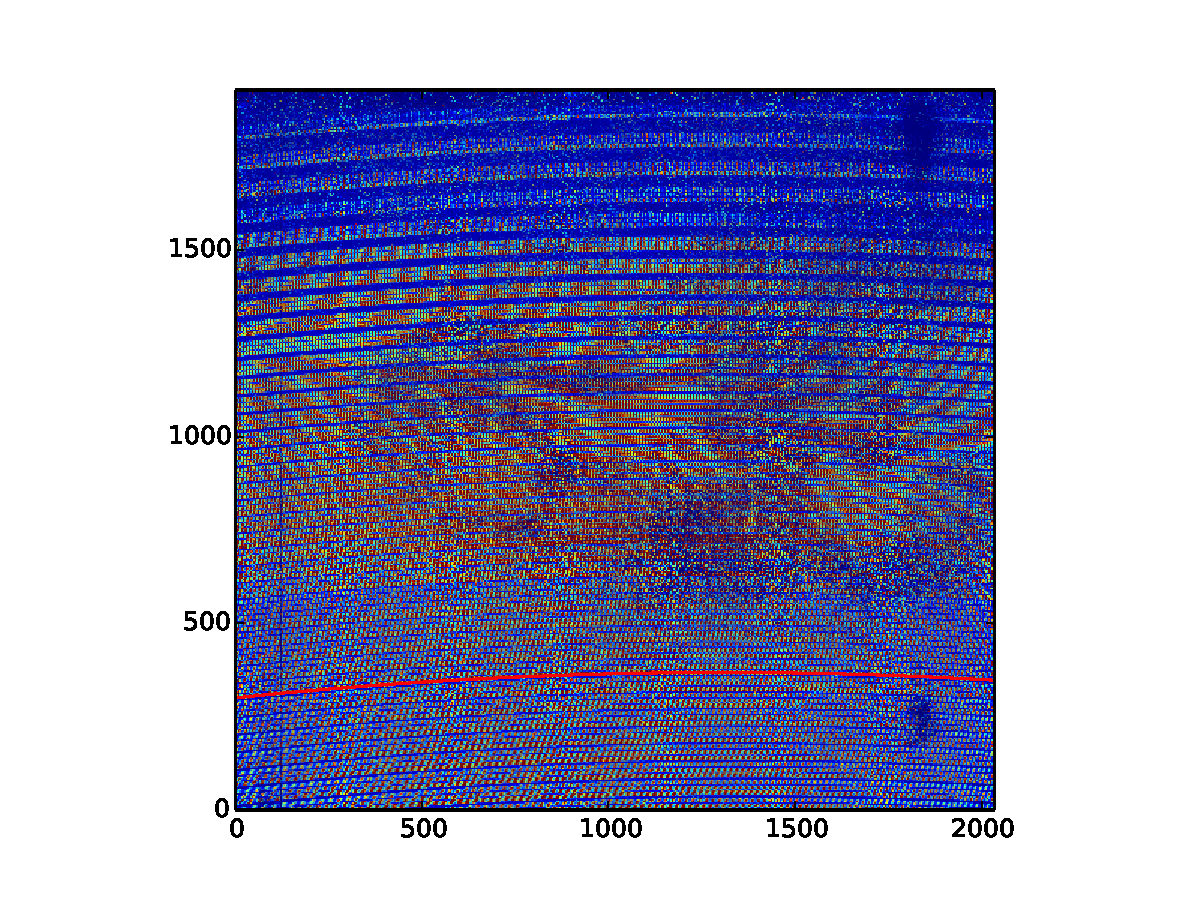
\includegraphics[width=.49\textwidth]{figures/cal_extract_RAW_spirou_1.pdf}}
\vcenteredhbox{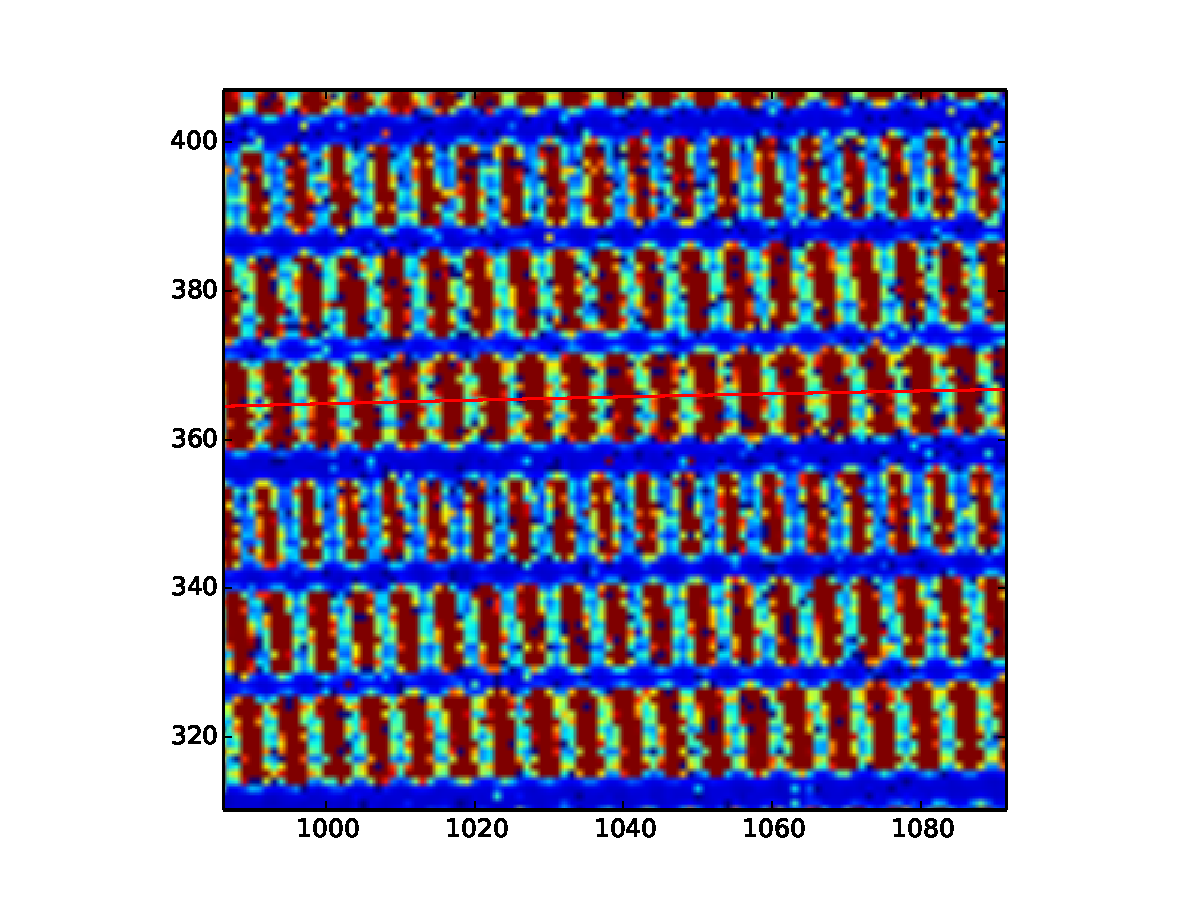
\includegraphics[width=.49\textwidth]{figures/cal_extract_RAW_spirou_1a.pdf}}
\caption{Left: The full process image. Right: Zoom in on the highlighted spectral order fit. \label{figure:cal_extract_RAW_spirou_1}}
\end{center}
\end{figure}

\begin{figure}
\begin{center}
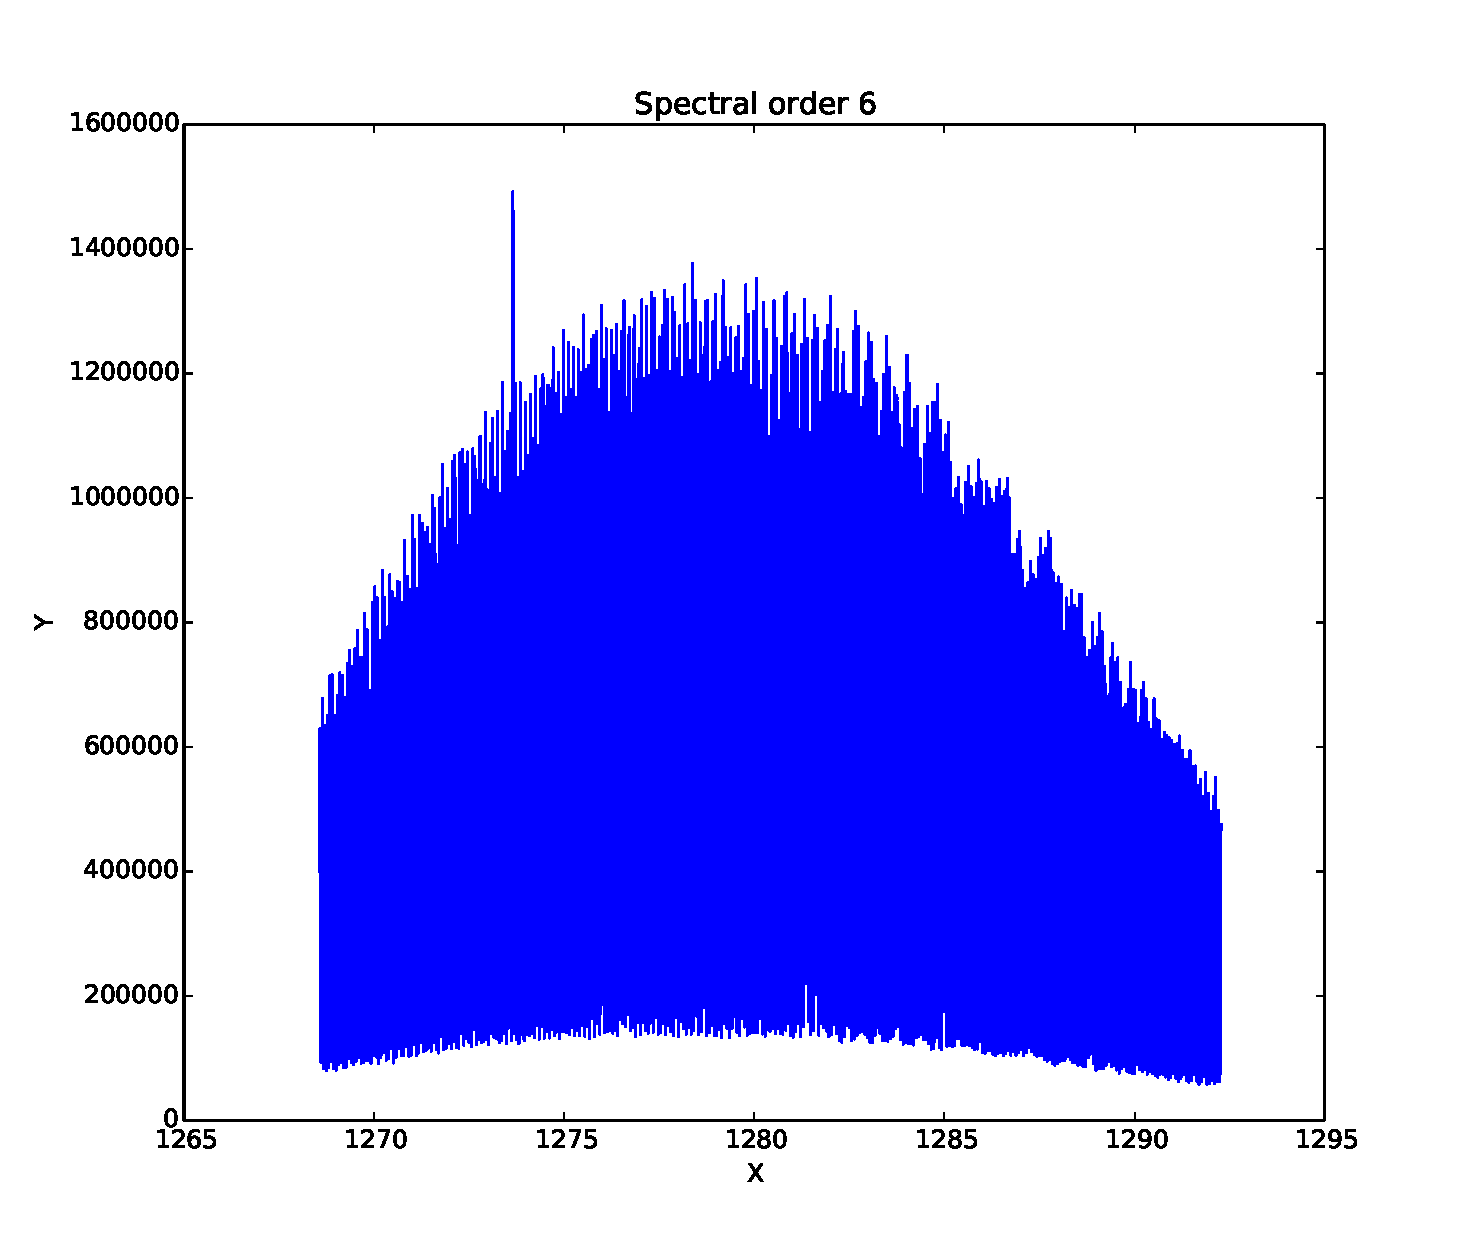
\includegraphics[width=.8\textwidth]{figures/cal_extract_RAW_spirou_2.pdf}
\caption{The extract spectrum from the hightlighted spectral order in \protect\ref{figure:cal_extract_RAW_spirou_1}. \label{figure:cal_extract_RAW_spirou_2}}
\end{center}
\end{figure}

% ----------------------------------------------------------------------------------
\clearpage
\newpage
\section{The cal\_DRIFT\_RAW\_spirou recipe}
\label{section:cal_DRIFT_RAW_spirou}
% ----------------------------------------------------------------------------------

Calculates relative (radial velocity) drift between all files and individual files. \\

% \TODO{Once writen up the new version update this description}

\noindent File prefixes allowed:
\begin{itemize}
	\item fp\_fp
\end{itemize}

\subsection{Summary of procedure}
\begin{enumerate}
	\item first file is reference image
	\item resizes the image
	\item extracts with weight (no tilt)
	\item loops around all other `fp\_fp' files in directory
	\item calculates photon noise uncertainty and estimated RV uncertainty on spectrum
	\begin{itemize}
		\item uses wave file
	\end{itemize}
	\item calculates RV drift and mean RV drift between reference (mean of files) and other `fp\_fp' files
	\item saves drift values to file
\end{enumerate}

\subsection{Running cal\_DRIFT\_RAW\_spirou}

To run cal\_DRIFT\_RAW\_spirou type:
\begin{lstlisting}[language=bash, style=bashstyle]
cal_DRIFT_RAW_spirou.py  night_repository  filenames
\end{lstlisting}

Note: Filenames must start with `fp\_fp'.

\subsection{Example working run}

An example run where everything worked is below:

\begin{lstlisting}[style=text]
cal_DRIFT_RAW_spirou.py 20170710 fp_fp02a203.fits fp_fp03a203.fits
fp_fp04a203.fits

||DRS  SPIROU   v   (interactive mode)
17:58:26.1 -   || *****************************************
17:58:26.1 -   || * SPIROU \@(#) Geneva Observatory ()
17:58:26.1 -   || *****************************************
17:58:26.1 -   ||(dir_data_raw)      DRS_DATA_RAW=/scratch/Projects/SPIRou_Pipeline/data/raw/
17:58:26.1 -   ||(dir_data_reduc)    DRS_DATA_REDUC=/scratch/Projects/SPIRou_Pipeline/data/reduced/
17:58:26.1 -   ||(dir_drs_config)    DRS_CONFIG=/scratch/Projects/SPIRou_Pipeline/INTROOT/DRS_SPIROU/config/
17:58:26.1 -   ||(dir_calib_db)      DRS_CALIB_DB=/scratch/Projects/SPIRou_Pipeline/data/calibDB
17:58:26.1 -   ||(dir_data_msg)      DRS_DATA_MSG=/scratch/Projects/SPIRou_Pipeline/data/msg/
17:58:26.1 -   ||(print_log)         DRS_LOG=1         %(0: minimum stdin-out logs)
17:58:26.1 -   ||(plot_graph)        DRS_PLOT=NONE            %(def/undef/trigger)
17:58:26.1 -   ||(used_date)         DRS_USED_DATE=undefined
17:58:26.1 -   ||(working_dir)       DRS_DATA_WORKING=/scratch/Projects/SPIRou_Pipeline/data/tmp/
17:58:26.1 -   ||                    DRS_INTERACTIVE is  set
17:58:26.1 -   |-c:+[...]|Now running : -c on file(s):  fp_fp02a203.fits fp_fp03a203.fits
17:58:26.1 -   |-c:+[...]|On directory /scratch/Projects/SPIRou_Pipeline/data/raw/20170710
17:58:26.1 -   |-c:+[...]|ICDP loaded from: /scratch/Projects/SPIRou_Pipeline/INTROOT/DRS_SPIROU/config/hadmrICDP_SPIROU.py
17:58:26.1 - * |-c:+[...]|Now processing Image TYPE: UNKNOWN  with -c recipe
17:58:26.2 -   |-c:+[...]|Calibration file: fp_fp02a203_tilt.fits already exists - not copied
17:58:26.2 -   |-c:+[...]|Calibration file: dark_flat02f10_loco_C.fits already exists - not copied
17:58:26.2 -   |-c:+[...]|Calibration file: flat_dark02f10_order_profil_AB.fits already exists - not copied
17:58:26.2 -   |-c:+[...]|Calibration file: spirou_wave_ini3.fits already exists - not copied
17:58:26.3 -   |-c:+[...]|Calibration file: dark_dark02d406.fits already exists - not copied
17:58:26.3 -   |-c:+[...]|Calibration file: dark_flat02f10_flat_C.fits already exists - not copied
17:58:26.3 -   |-c:+[...]|Calibration file: dark_flat02f10_order_profil_C.fits already exists - not copied
17:58:26.3 -   |-c:+[...]|Calibration file: flat_dark02f10_loco_AB.fits already exists - not copied
17:58:26.3 -   |-c:+[...]|Reading File: /scratch/Projects/SPIRou_Pipeline/data/raw/20170710/fp_fp02a203.fits
17:58:26.3 -   |-c:+[...]|Image 2048x2048 loaded
17:58:26.4 -   |-c:+[...]|Doing Dark Correction using /scratch/Projects/SPIRou_Pipeline/data/calibDB/dark_dark02d406.fits
17:58:26.8 -   |-c:+[...]|Image format changed to 2035x1930
17:58:27.2 - * |-c:+[...]|Nb pixels morts = 600284 / 15.28 %
17:58:27.2 -   |-c:+[...]|Reading tilt slit 
17:58:27.2 -   |-c:+[...]AB|Reading localization parameters of Fiber AB
17:58:27.3 -   |-c:+[...]AB|Reading order profil of Fiber AB
17:58:27.3 -   |-c:+[...]|Reading wavelength solution 
17:58:27.3 -   |-c:+[...]|Extraction Reference file  /scratch/Projects/SPIRou_Pipeline/data/raw/20170710/fp_fp02a203.fits
17:58:27.4 -   |-c:+[...]|On fiber AB  order  0: S/N= 513.5  
17:58:27.6 -   |-c:+[...]|On fiber AB  order  1: S/N= 561.6  
17:58:27.7 -   |-c:+[...]|On fiber AB  order  2: S/N= 525.8  
17:58:27.9 -   |-c:+[...]|On fiber AB  order  3: S/N= 520.4  
17:58:28.0 -   |-c:+[...]|On fiber AB  order  4: S/N= 518.1  
17:58:28.1 -   |-c:+[...]|On fiber AB  order  5: S/N= 549.3  
17:58:28.3 -   |-c:+[...]|On fiber AB  order  6: S/N= 590.9  
17:58:28.4 -   |-c:+[...]|On fiber AB  order  7: S/N= 574.5  
17:58:28.6 -   |-c:+[...]|On fiber AB  order  8: S/N= 582.1  
17:58:28.7 -   |-c:+[...]|On fiber AB  order  9: S/N= 592.4  
17:58:28.9 -   |-c:+[...]|On fiber AB  order 10: S/N= 615.4  
17:58:29.0 -   |-c:+[...]|On fiber AB  order 11: S/N= 525.9  
17:58:29.2 -   |-c:+[...]|On fiber AB  order 12: S/N= 697.1  
17:58:29.3 -   |-c:+[...]|On fiber AB  order 13: S/N= 735.1  
17:58:29.5 -   |-c:+[...]|On fiber AB  order 14: S/N= 920.8  
17:58:29.6 -   |-c:+[...]|On fiber AB  order 15: S/N= 830.5  
17:58:29.8 -   |-c:+[...]|On fiber AB  order 16: S/N= 818.3  
17:58:29.9 -   |-c:+[...]|On fiber AB  order 17: S/N= 840.0  
17:58:30.1 -   |-c:+[...]|On fiber AB  order 18: S/N= 814.2  
17:58:30.2 -   |-c:+[...]|On fiber AB  order 19: S/N= 829.1  
17:58:30.4 -   |-c:+[...]|On fiber AB  order 20: S/N= 836.1  
17:58:30.5 -   |-c:+[...]|On fiber AB  order 21: S/N= 826.4  
17:58:30.7 -   |-c:+[...]|On fiber AB  order 22: S/N= 812.6  
17:58:30.8 -   |-c:+[...]|On fiber AB  order 23: S/N= 828.2
17:58:31.0 -   |-c:+[...]|On fiber AB  order 24: S/N= 785.1
17:58:31.1 -   |-c:+[...]|On fiber AB  order 25: S/N= 770.6
17:58:31.3 -   |-c:+[...]|On fiber AB  order 26: S/N= 743.6
17:58:31.4 -   |-c:+[...]|On fiber AB  order 27: S/N= 758.9
17:58:31.6 -   |-c:+[...]|On fiber AB  order 28: S/N= 765.8
17:58:31.7 -   |-c:+[...]|On fiber AB  order 29: S/N= 685.6
17:58:31.9 -   |-c:+[...]|On fiber AB  order 30: S/N= 612.8
17:58:32.0 -   |-c:+[...]|On fiber AB  order 31: S/N= 307.0
17:58:32.2 -   |-c:+[...]|On fiber AB  order 32: S/N= 255.6
17:58:32.3 -   |-c:+[...]|On fiber AB  order 33: S/N= 355.5
17:58:32.5 -   |-c:+[...]|On fiber AB  order 34: S/N= 283.3
17:58:32.6 -   |-c:+[...]|On fiber AB  order 35: S/N= 149.9
17:58:32.9 - * |-c:+[...]|On fiber AB estimated RV uncertainty on spectrum is 0.028 m/s
17:58:32.9 - * |-c:+[...]|Nb fp_fp files found on directory =  2
17:58:32.9 -   |-c:+[...]|Reading File: /scratch/Projects/SPIRou_Pipeline/data/raw/20170710/fp_fp03a203.fits
17:58:39.3 -   |-c:+[...]|Time from ref= 0.09 h  - Drift mean= 2.53 m/s - Flux ratio= 0.99 - Nb Cosmics= 1218
17:58:39.3 -   |-c:+[...]|Reading File: /scratch/Projects/SPIRou_Pipeline/data/raw/20170710/fp_fp04a203.fits
17:58:45.6 -   |-c:+[...]|Time from ref= 0.18 h  - Drift mean= -10.14 m/s - Flux ratio= 0.98 - Nb Cosmics= 1246
17:58:45.6 -   |-c:+[...]|Total drift Peak-To-Peak= 12.607 m/s RMS= 5.201 m/s in 0.00 hour
17:58:45.6 -   |-c:+[...]|Saving drift values of Fiber AB in fp_fp02a203_drift_AB.fits
17:58:45.8 - * |-c:+[...]|Recipe -c has been  successfully completed
\end{lstlisting}

\subsection{Interactive mode}

\begin{figure}
\begin{center}
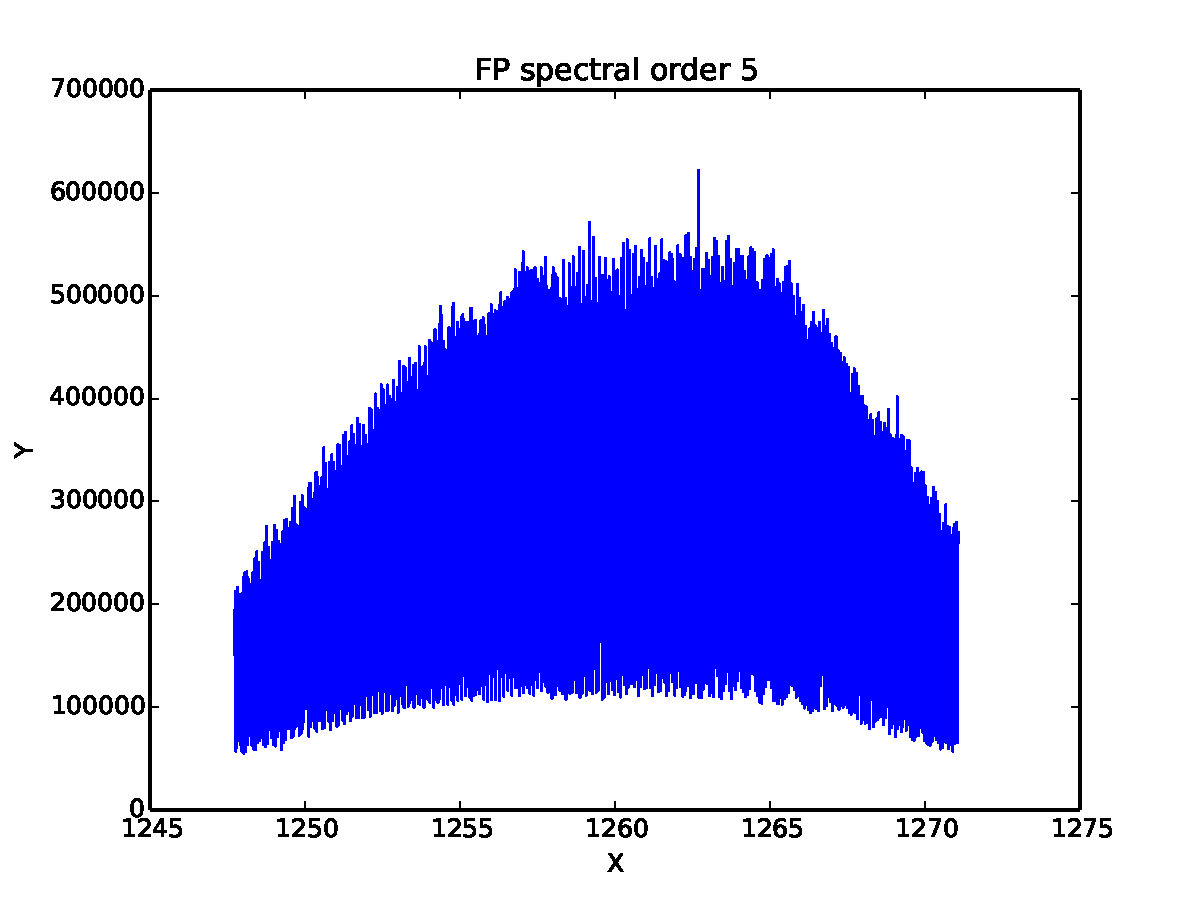
\includegraphics[width=.8\textwidth]{figures/cal_DRIFT_RAW_spirou_1}
\caption{Extract FP spectral order. \label{figure:cal_DRIFT_RAW_spirou_1}}
\end{center}
\end{figure}

\begin{figure}
\begin{center}
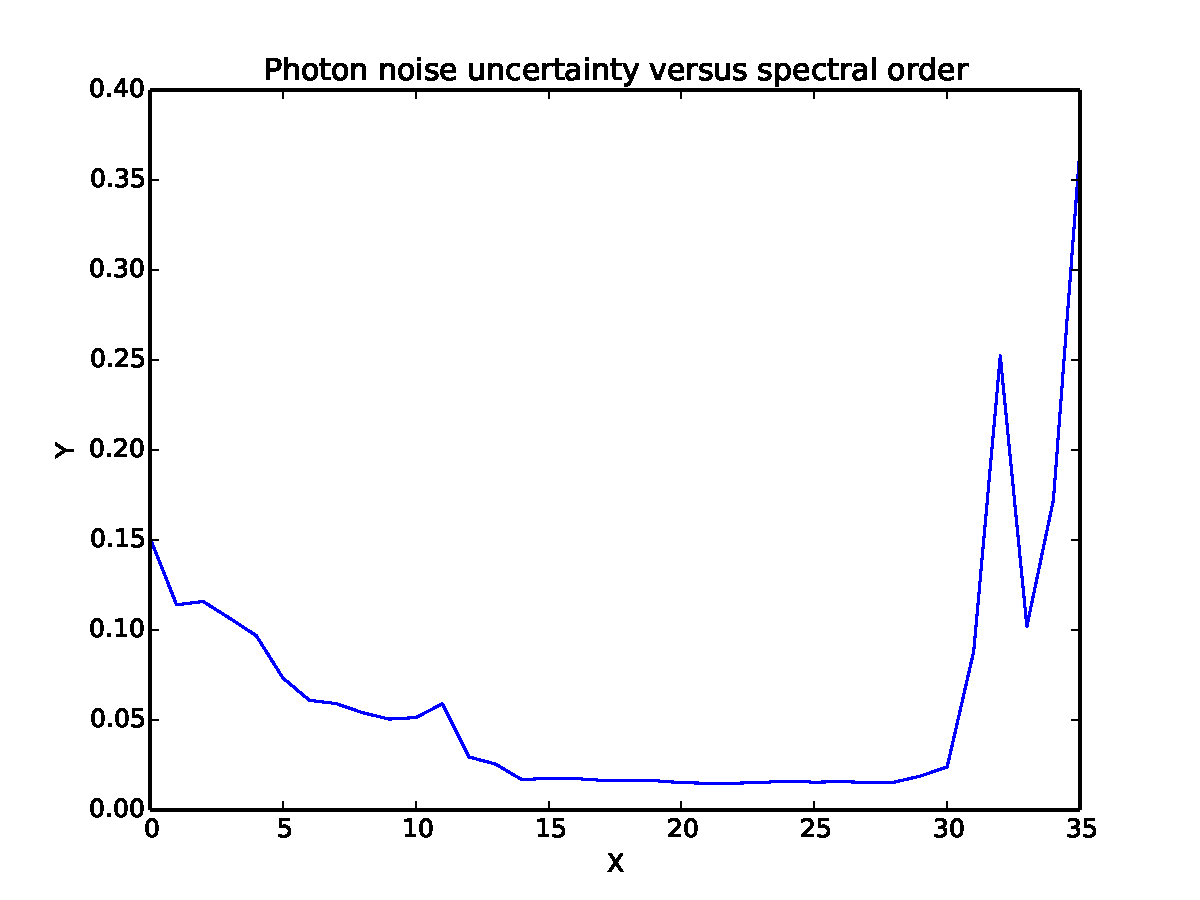
\includegraphics[width=.8\textwidth]{figures/cal_DRIFT_RAW_spirou_2}
\caption{Photon noise uncertain against spectral order. \label{figure:cal_DRIFT_RAW_spirou_2}}
\end{center}
\end{figure}

\begin{figure}
\begin{center}
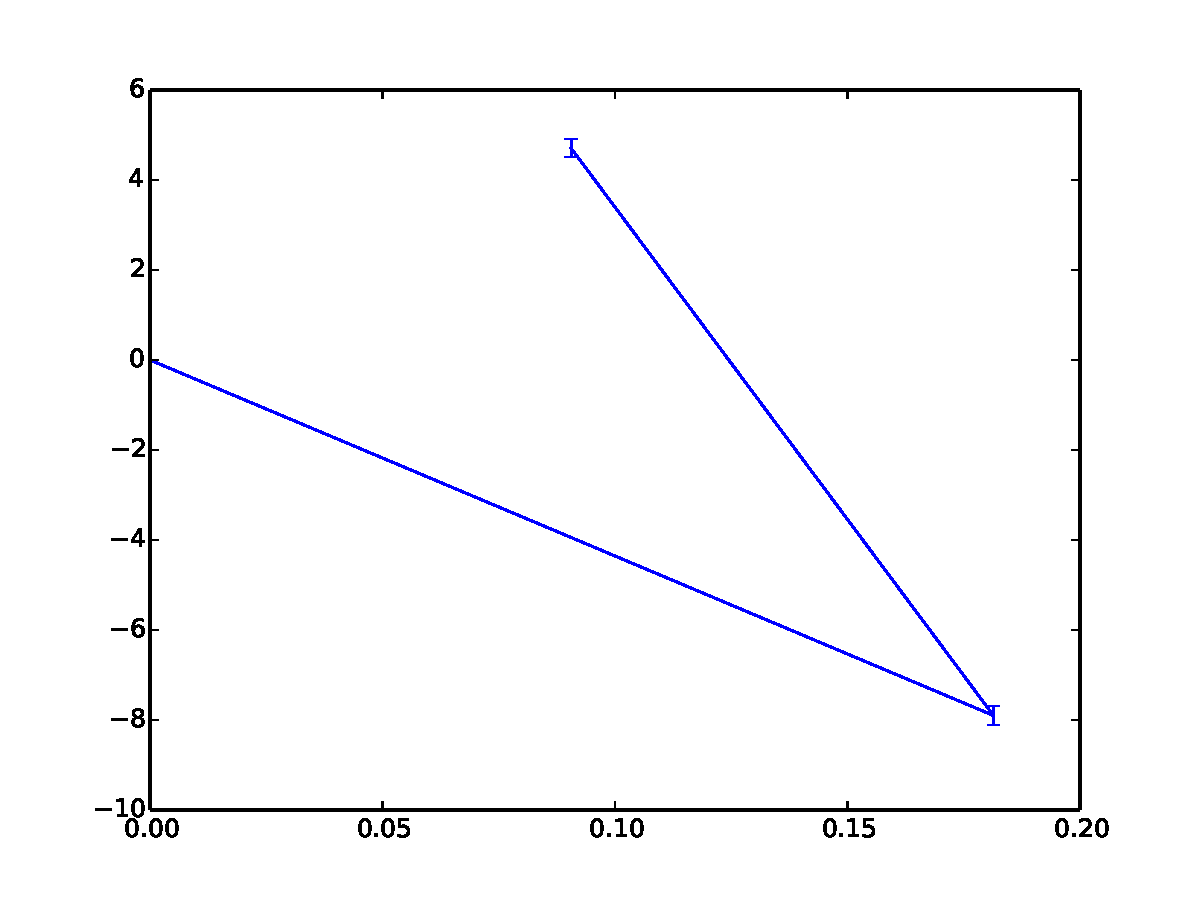
\includegraphics[width=.8\textwidth]{figures/cal_DRIFT_RAW_spirou_3}
\caption{Time interval against median drift. \label{figure:cal_DRIFT_RAW_spirou_3}}
\end{center}
\end{figure}



%----------------------------------------------------------------------------------
\clearpage
\newpage
\section{The cal\_HC\_E2DS\_spirou recipe}
\label{section:cal_HC_E2DS}
% ----------------------------------------------------------------------------------

Wavelength calibration. \\

% % \TODO{Once writen up the new version update this description}

\noindent File prefixes allowed:
\begin{itemize}
	\item hc\_hc*AB.fits
	\item hc\_hc*C.fits
\end{itemize}

\subsection{Summary of procedure}
\begin{enumerate}
	\item Reads lamp line file
	\item Tries to identify lines using guess solution
	\item Cleans list of identified lines
	\item Fits wavelength solution on identified lines
	\item Performs a Littrow test
	\item Writes wavelength solution for fibers
	\item Computes CCF
\end{enumerate}

\subsection{Running cal\_HC\_E2DS\_spirou}

To run cal\_HC\_E2DS\_spirou type:
\begin{lstlisting}[language=bash, style=bashstyle]
cal_HC_E2DS_spirou.py  night_repository  hc_hc*.fits
\end{lstlisting}

\noindent Note: Filenames must start with hc\_hc
\noindent Note: Filenames must include either AB or C

% \subsection{Example working run}

% An example run where everything worked is below:

% \begin{lstlisting}[style=text]
% cal_ .py 20170710 
% \end{lstlisting}

% \subsection{Interactive mode}

% \begin{figure}
% \begin{center}
% \includegraphics[width=.8\textwidth]{figures/}
% \caption{ \label{}}
% \end{center}
% \end{figure}

% ----------------------------------------------------------------------------------
\clearpage
\newpage
\section{The cal\_DRIFT-PEAK\_E2DS\_spirou recipe}
\label{section:cal_}
% ----------------------------------------------------------------------------------

Calculates relative (radial velocity) drift between all files and individual files using a gaussian fitting process to fit the FP peaks. \\

% \TODO{Once writen up the new version update this description}

\noindent File prefixes allowed:
\begin{itemize}
	\item fp\_fp
\end{itemize}

\subsection{Summary of procedure}
\begin{enumerate}
	\item first file is reference image
	\item resizes the image
	\item background correction
	\item Identifies FP peaks in reference file
	\item Creates a reference ascii file that contains the positions of the FP peaks
	\item Removes lines with suspicious widths
	\item loops around all other *\_e2ds\_\definevariable{fiber}.fits files
	\item Gets the centroid of all peaks using Gaussian fitting
	\item Performs a Pearson R test to look for issues with extraction and/or illumination
	\item Performs sigma clipping on measured drift
	\item Saves drifts to file
\end{enumerate}

\subsection{Running cal\_DRIFT-PEAK\_E2DS\_spirou}

To run cal\_DRIFT-PEAK\_E2DS\_spirou type:
\begin{lstlisting}[language=bash, style=bashstyle]
cal_DRIFT-PEAK_E2DS_spirou.py  night_repository fp_fp*.fits
\end{lstlisting}

\noindent Note: Filenames must start with fp\_fp.

% \subsection{Example working run}

% An example run where everything worked is below:

% \begin{lstlisting}[style=text]
% cal_DRIFT-PEAK_E2DS_spirou.py  20170710 
% \end{lstlisting}

% \subsection{Interactive mode}

% \begin{figure}
% \begin{center}
% \includegraphics[width=.8\textwidth]{figures/}
% \caption{ \label{}}
% \end{center}
% \end{figure}


% ----------------------------------------------------------------------------------
\clearpage
\newpage
\section{The cal\_WAVE\_E2DS\_spirou recipe}
\label{section:cal_WAVE_E2DS_spirou}
% ----------------------------------------------------------------------------------

New wavelength solution combining Hollow-Cathode + FP E2DS spectra. \\

% % \TODO{Once writen up the new version update this description}

\noindent File prefixes allowed:
\begin{itemize}
	\item hc\_hc (first file)
	\item fp\_fp (second file)
\end{itemize}

\subsection{Summary of procedure}
\begin{enumerate}
	\item Reads lamp line file
	\item Performs instrumental drift computation
	\item Writes drift to e2ds fits file
	\item Calculates initial wavelength solution
	\item Tries to identify lines using guess solution (x2) 
	\item Cleans list of identified lines (x2)
	\item Fits wavelength solution on identified lines (x2)
	\item Performs a Littrow test (x2)
	\item Writes wavelength solution for fibers
	\item Computes CCF
\end{enumerate}

\subsection{Running cal\_WAVE\_E2DS\_spirou}

To run cal\_WAVE\_E2DS\_spirou type:
\begin{lstlisting}[language=bash, style=bashstyle]
cal_WAVE_E2DS_spirou.py night_repository  hc_hc_*_e2ds_AB.fits    fp_fp_*_e2ds_AB.fits 
\end{lstlisting}

\noindent Note: First file must start with hc\_hc and contain AB or C
\noindent Note: Second file must start with fp\_fp and contain AB or C

% \subsection{Example working run}

% An example run where everything worked is below:

% \begin{lstlisting}[style=text]
% cal_ .py 20170710 
% \end{lstlisting}

% \subsection{Interactive mode}

% \begin{figure}
% \begin{center}
% \includegraphics[width=.8\textwidth]{figures/}
% \caption{ \label{}}
% \end{center}
% \end{figure}


% ----------------------------------------------------------------------------------
\clearpage
\newpage
\section{The cal\_BADPIX\_spirou recipe}
\label{section:cal_BADPIX_spirou}
% ----------------------------------------------------------------------------------

Recipe to generate the bad pixel map. \\

% \TODO{Once writen up the new version update this description}

\noindent File prefixes allowed:
\begin{itemize}
	\item flat\_flat (first file)
	\item dark\_dark (second file)
\end{itemize}

\subsection{Summary of procedure}
\begin{enumerate}
	\item Normalise the flats
	\item Look for isolated hot pixels
	\item Calculate how much pixels deviate compared to expected values
	\item Select hot pixels compared to neighbours
	\item Combine bad pixel map
	\item Save bad pixel mask to file
\end{enumerate}

\subsection{Running cal\_DRIFT\_RAW\_spirou}

To run cal\_DRIFT\_RAW\_spirou type:
\begin{lstlisting}[language=bash, style=bashstyle]
cal_BADPIX_spirou.py night_repository flat_flat*.fits dark_dark*.fits
\end{lstlisting}

\noindent Note: Filenames must start with flat\_flat (first file) and dark\_dark (second file)

\noindent Note: only two files allowed (one flat plus one dark)

\subsection{Example working run}

An example run where everything worked is below:

\begin{lstlisting}[style=text]
cal_BADPIX_spirou.py 20170710 flat_flat02f10.fits dark_dark02d406.fits
||DRS  SPIROU   v   (interactive mode)
15:49:54.7 -   || *****************************************
15:49:54.7 -   || * SPIROU \@(#) Geneva Observatory ()
15:49:54.7 -   || *****************************************
15:49:54.7 -   ||(dir_data_raw)      DRS_DATA_RAW=/scratch/Projects/SPIRou_Pipeline/data/raw/
15:49:54.7 -   ||(dir_data_reduc)    DRS_DATA_REDUC=/scratch/Projects/SPIRou_Pipeline/data/reduced/
15:49:54.7 -   ||(dir_drs_config)    DRS_CONFIG=/scratch/Projects/SPIRou_Pipeline/INTROOT/DRS_SPIROU/config/
15:49:54.7 -   ||(dir_calib_db)      DRS_CALIB_DB=/scratch/Projects/SPIRou_Pipeline/data/calibDB
15:49:54.7 -   ||(dir_data_msg)      DRS_DATA_MSG=/scratch/Projects/SPIRou_Pipeline/data/msg/
15:49:54.7 -   ||(print_log)         DRS_LOG=1         %(0: minimum stdin-out logs)
15:49:54.7 -   ||(plot_graph)        DRS_PLOT=1            %(def/undef/trigger)
15:49:54.7 -   ||(used_date)         DRS_USED_DATE=undefined
15:49:54.7 -   ||(working_dir)       DRS_DATA_WORKING=/scratch/Projects/SPIRou_Pipeline/data/tmp/
15:49:54.7 -   ||                    DRS_INTERACTIVE is  set
15:49:54.7 -   |cal_BADPIX_spirou:+[...]|Now running : cal_BADPIX_spirou on file(s):  flat_flat02f10.fits dark_dark02d406.fits
15:49:54.7 -   |cal_BADPIX_spirou:+[...]|On directory /scratch/Projects/SPIRou_Pipeline/data/raw/20170710
15:49:54.7 -   |cal_BADPIX_spirou:+[...]|ICDP loaded from: /scratch/Projects/SPIRou_Pipeline/INTROOT/DRS_SPIROU/config/hadmrICDP_SPIROU.py
15:49:54.7 - * |cal_BADPIX_spirou:+[...]|Now processing Image TYPE FLAT with cal_BADPIX_spirou recipe
15:49:54.7 - * |cal_BADPIX_spirou:+[...]|Now processing Image TYPE DARK with cal_BADPIX_spirou recipe
15:49:54.7 -   |cal_BADPIX_spirou:+[...]|Reading Flat Image /scratch/Projects/SPIRou_Pipeline/data/raw/20170710/flat_flat02f10.fits
15:49:54.7 -   |cal_BADPIX_spirou:+[...]|Flat Image 2048x2048 loaded
15:49:54.7 -   |cal_BADPIX_spirou:+[...]|Reading Dark Image /scratch/Projects/SPIRou_Pipeline/data/raw/20170710/flat_flat02f10.fits
15:49:54.8 -   |cal_BADPIX_spirou:+[...]|Dark Image 2048x2048 loaded
15:49:54.8 -   |cal_BADPIX_spirou:+[...]|Normalising the flat image
15:49:55.9 -   |cal_BADPIX_spirou:+[...]|Looking for bad pixels
15:49:56.9 -   |cal_BADPIX_spirou:+[...]|Fraction of hot pixels from dark: 3.01 %
15:49:56.9 -   |cal_BADPIX_spirou:+[...]|Fraction of bad pixels from flat: 1.32 %
15:49:56.9 -   |cal_BADPIX_spirou:+[...]|Fraction of NaN pixels in dark: 20.76 %
15:49:56.9 -   |cal_BADPIX_spirou:+[...]|Fraction of NaN pixels in flat: 14.66 %
15:49:56.9 -   |cal_BADPIX_spirou:+[...]|Fraction of bad pixels with all criteria: 24.66 %
15:49:56.9 - * |cal_BADPIX_spirou:+[...]|QUALITY CONTROL SUCCESSFUL - Well Done -
15:49:56.9 -   |cal_BADPIX_spirou:+[...]|Saving Bad Pixel Mask in flat_flat02f10_badpixel.fits
15:49:57.5 - * |cal_BADPIX_spirou:+[...]|Updating Calib Data Base with BADPIX
15:49:57.5 - * |cal_BADPIX_spirou:+[...]|Recipe cal_BADPIX_spirou has been succesfully completed
\end{lstlisting}


% ----------------------------------------------------------------------------------
\clearpage
\newpage
\section{The cal\_CCF\_E2DS\_spirou recipe}
\label{section:cal_CCF_E2DS_spirou}
% ----------------------------------------------------------------------------------

Cross correlation function computation on a E2DS spectra. \\

% \TODO{Once writen up the new version update this description}

\noindent File suffixes allowed:
\begin{itemize}
	\item *e2ds\_AB.fits
\end{itemize}

\subsection{Summary of procedure}
\begin{enumerate}
	\item 
\end{enumerate}

\subsection{Running cal\_DRIFT\_RAW\_spirou}

To run cal\_DRIFT\_RAW\_spirou type:
\begin{lstlisting}[language=bash, style=bashstyle]
cal_CCF_E2DS_spirou.py  night_repository  *e2ds_AB.fits  mask.mas  RV  RANGE  STEP 
\end{lstlisting}

\noindent Note: First argument is a file with suffix *e2ds\_AB.fits
\noindent Note: The mask (Ex : UrNe.mas) is presently loaded locally (in the working directory) 
\noindent Note: RV, RANGE, STEP are the central velocity, half range in velocity and step in km/s of the CCF 

% \subsection{Example working run}

% An example run where everything worked is below:

% \begin{lstlisting}[style=text]
% cal_ .py 20170710 
% \end{lstlisting}

% \subsection{Interactive mode}

% \begin{figure}
% \begin{center}
% \includegraphics[width=.8\textwidth]{figures/}
% \caption{ \label{}}
% \end{center}
% \end{figure}


% % ----------------------------------------------------------------------------------
% \clearpage
% \newpage
% \section{The cal\_ recipe}
% \label{section:cal_}
% % ----------------------------------------------------------------------------------



% % \TODO{Once writen up the new version update this description}

% \noindent File prefixes allowed:
% \begin{itemize}
% 	\item 
% \end{itemize}

% \subsection{Summary of procedure}
% \begin{enumerate}
% 	\item 
% \end{enumerate}

% \subsection{Running cal\_DRIFT\_RAW\_spirou}

% To run cal\_DRIFT\_RAW\_spirou type:
% \begin{lstlisting}[language=bash, style=bashstyle]
% cal_ .py  night_repository  filenames
% \end{lstlisting}

% Note: Filenames must start with 

% \subsection{Example working run}

% An example run where everything worked is below:

% \begin{lstlisting}[style=text]
% cal_ .py 20170710 
% \end{lstlisting}

% \subsection{Interactive mode}

% \begin{figure}
% \begin{center}
% \includegraphics[width=.8\textwidth]{figures/}
% \caption{ \label{}}
% \end{center}
% \end{figure}

% ---------------------------------------------------------------
\clearpage
\newpage
\section{Currently unused}
% ---------------------------------------------------------------

\subsection{cal\_loc\_ONE\_spirou}

White lamp exposures on fiber science only (A and B), on fiber C only, or on all of them (ABC). These exposures are used for order localisation and order profil (the pipeline will also need a Fabry-Perot exposure for this last point).

\subsubsection{Running cal\_loc\_ONE\_spirou}

To run cal\_loc\_ONE\_spirou type:
\begin{lstlisting}[language=bash, style=bashstyle]
cal_loc_ONE_spirou.py  night_repository  filename
\end{lstlisting}


\subsection{cal\_FF\_spirou}

A sequence of N white lamp exposures where the two fibres are simultaneously illuminated. This sequence is used by the data reduction pipeline for producing a spectral "master flat-field", monitor the ageing of detector (IR detector loose pixels during its life), monitor the fiber transmission, produce localisation and order profil (the pipeline will also need of exposure « Fabry-Perot » for this last point).

\subsubsection{Running cal\_FF\_spirou}

To run cal\_FF\_spirou type:
\begin{lstlisting}[language=bash, style=bashstyle]
cal_FF_spirou.py  night_repository  filename1 filename2 … filenameN
\end{lstlisting}


\subsection{cal\_WAVE\_spirou}

Hollow Cathode lamp exposures in which the three fibres are simultaneously fed by light from the Hollow Cathode lamps. DRS use each exposure to build a wavelength solution. The instrumental drift with respect to the previous calibration frames is measured.

\subsubsection{Running cal\_WAVE\_spirou}

To run cal\_WAVE\_spiroutype:
\begin{lstlisting}[language=bash, style=bashstyle]
cal_WAVE_spirou.py  night_repository  filename
\end{lstlisting}



\subsection{cal\_FP\_spirou}

Fabry-Perot exposures in which the three fibres are simultaneously fed by light from the Fabry-Perot filter. Each exposure is used to build a wavelength solution and the slit orientation. The instrumental drift with respect to the previous calibration frames is measured. A « super » wavelength solution will be builded in using Hollow Cathode and Fabry-Perot exposures; Hollow Cathode exposures give an absolute reference and Fabry-Perot exposures provide a signal very regularly spaced  in wavelength.

\subsubsection{Running cal\_FP\_spirou}

To run cal\_FP\_spirou type:
\begin{lstlisting}[language=bash, style=bashstyle]
cal_FP_spirou.py  night_repository  filename
\end{lstlisting}


%Chapeter 6: Quality Control
 \chapter{Quality Control}


\section{cal\_DARK\_spirou}
\label{section:qc_cal_DARK_spirou}

There are currently two quality control checks for cal\_DARK\_spirou
\begin{itemize}
\item Unexpected dark level: $\text{Median Flux} < QC_{\text{Max Dark Level}}$
\item Unexpected Fraction of dead pixels: $\text{Number of dead pixels} < QC_{\text{Max Dead Pixels}}$
\end{itemize}

where $QC_{\text{Max Dark Level}}$ and $QC_{\text{Max Dead Pixels}}$ are constants currently defined in cal\_DARK\_spirou.py
\begin{lstlisting}[style=pythonstyle]
##########################
#   Quality control      #
##########################

qc_max_darklevel=1.0  # Max dark median level [ADU/s]  
qc_maxdead=25.0       # Fraction Max of dead pixel [%]
\end{lstlisting}

\section{cal\_loc\_RAW\_spirou}
\label{section:qc_cal_loc_RAW_spirou}

Some text here

\section{cal\_SLIT\_spirou}
\label{section:qc_cal_SLIT_spirou}

Some text here

\section{cal\_FF\_RAW\_spirou}
\label{section:qc_cal_FF_RAW_spirou}

Some text here

\section{cal\_extract\_RAW\_spirou}
\label{section:qc_cal_extract_RAW_spirou}

Some text here

\section{cal\_DRIFT\_RAW\_spirou}
\label{section:qc_cal_DRIFT_RAW_spirou}

Some text here

% Appendix
\appendix

% Appendix A: env_setup.sh
\chapter{Source code for env\_setup.sh}
\label{section:source_code_env_setup_sh}

Below is the source code for `env\_setup.sh' and should be saved as `env\_setup.sh' and be allowed to execute:
\begin{lstlisting}[style=bashstyle]
chmod +x env_setup.sh
\end{lstlisting}

\begin{lstlisting}[style=text]
#!/bin/bash
# alias.sh

# Use --clean to restore environment

# --------------------------------------------------------------------
# EDIT THESE PARAMETERS
# --------------------------------------------------------------------
# Set the instrument name
INSTRUMENT_NAME="SPIROU"
# Directory in which all SPIROU files go
DIR="/data/spirou/drs/"
# Define installation folder name
INSTALL_ROOT="$DIR/INTROOT"
# Define data folder name
DATA_ROOT="$DIR/data"
# Define raw path
DATA_ROOT_RAW="$DATA_ROOT/raw/"
# Define reduced path
DATA_ROOT_REDUCED="$DATA_ROOT/reduced/"
# Define calibDB path
DATA_ROOT_CALIB="$DATA_ROOT/calibDB"
# Define msg path
DATA_ROOT_MSG="$DATA_ROOT/msg/"
# Define tmp path
DATA_ROOT_TMP="$DATA_ROOT/tmp/"
# Define whether to run interactive session
INTERACTIVE=1
# Define python version
PYTHON_VERSION="2.7"
# Define python directory (i.e. result of command "which python")
PYTHON_DIR="$DIR/python/miniconda2"
# Define GSL path
GSL_DIR="$DIR/c-libraries/gsl"


# --------------------------------------------------------------------
# DO NOT EDIT PAST THIS POINT
# --------------------------------------------------------------------
echo " ========================================= "
echo "  Environmental setup for DRS Pipeline     "
echo " ========================================= "

# get arguments
CLEAN="0"
for i in "$\@"; do
  case $i in 
    --clean) CLEAN="1";;
    *) echo "Invalid argument"; exit 1;;
  esac
done

if [ "$CLEAN" = "1" ]; then
  if [[ -z "${DRS_ACTIVE}" ]]; then
    if [ "$DRS_ACTIVE" != 1 ]; then
      echo "   No need to clean - environment clean"
      echo ""
      echo "   Done"
      exit
    fi
  fi
  echo "   Cleaning environment"
  export PATH=$OLDPATH
  export PYTHONPATH=$OLDPYTHONPATH
  unset OLDPATH
  unset DRS_ACTIVE
  unset OLDPYTHONPATH
  unset INTROOT
  unset DRS_LOG
  unset PYTHON_INCLUDE_DIR
  unset GSL_INCLUDE_DIR
  unset GSL_LIBRARY_DIR
  unset INSTRUMENT
  unset DRS_DATA_RAW
  unset DRS_DATA_REDUC
  unset DRS_CALIB_DB
  unset DRS_DATA_MSG
  unset DRS_DATA_WORKING
  unset TDATA
  unset DRS_INTERACTIVE
  unalias conda
  unalias pip
  unalias f2py
else
  echo "   Setting up environment"
  # Backup old path and python path for clean
  OLDPATH=$PATH
  OLDPYTHONPATH=$PYTHONPATH
  export OLDPATH
  export DRS_ACTIVE=1
  export OLDPYTHONPATH
  
  #User specific environment and startup programs
  export INTROOT="$INSTALL_ROOT"
  export PATH=.:"$INSTALL_ROOT/bin":"$PYTHON_DIR/bin":$PATH
  export PYTHONPATH=.:"$PYTHON_DIR/lib/python$PYTHON_VERSION/site-packages/":"$INSTALL_ROOT/bin/"
  export DRS_LOG=1
  export PYTHON_INCLUDE_DIR="$PYTHON_DIR/lib/python$PYTHON_VERSION/site-packages/numpy/core/include"
  export GSL_INCLUDE_DIR="$GSL_DIR/include"
  export GSL_LIBRARY_DIR="$GSL_DIR/lib"
  # force aliases
  chmod +x "$PYTHON_DIR/bin/conda"
  alias conda="$PYTHON_DIR/bin/conda"
  chmod +x "$PYTHON_DIR/bin/pip"
  alias pip="$PYTHON_DIR/bin/pip"
  chmod +x "$PYTHON_DIR/bin/f2py"
  alias f2py="$PYTHON_DIR/bin/f2py"
  
  #SPIROU DRS and DATA environment variables
  export INSTRUMENT=$INSTRUMENT_NAME
  export DRS_DATA_RAW=$DATA_ROOT_RAW
  export DRS_DATA_REDUC=$DATA_ROOT_REDUCED
  export DRS_CALIB_DB=$DATA_ROOT_CALIB
  export DRS_DATA_MSG=$DATA_ROOT_MSG
  export DRS_DATA_WORKING=$DATA_ROOT_TMP
  export DRS_INTERACTIVE=$INTERACTIVE
  export TDATA=$DATA_ROOT
  
  echo "   Set up for $INSTRUMENT"
  echo "    - Python located at: $PYTHON_DIR"
  echo "    - GLS located at: $GSL_DIR"
  echo "    - installation located at: $INSTALL_ROOT"
  echo "    - data located at:"
  echo "           $DATA_ROOT"
  echo "           $DATA_ROOT_RAW"
  echo "           $DATA_ROOT_REDUCED"
  echo "           $DATA_ROOT_CALIB"
  echo "           $DATA_ROOT_MSG"
  echo "           $DATA_ROOT_TMP"
  echo " "
  
fi

echo "   Done"
\end{lstlisting}  

%%%-------------------------------------------------------------------------------

\backmatter

%%% BIBLIOGRAPHY
%%% -------------------------------------------------------------

% \bibliographystyle{utphysics}
% \bibliography{ref}

\end{document}